%%%%%%%%%%%%%%%%%%%%%%%%%%%%%%%%%%%%%%%%%
% The Legrand Orange Book
% LaTeX Template
% Version 2.1.1 (14/2/16)
%
% This template has been downloaded from:
% http://www.LaTeXTemplates.com
%
% Original author:
% Mathias Legrand (legrand.mathias@gmail.com) with modifications by:
% Vel (vel@latextemplates.com)
%
% License:
% CC BY-NC-SA 3.0 (http://creativecommons.org/licenses/by-nc-sa/3.0/)
%
% Compiling this template:
% This template uses biber for its bibliography and makeindex for its index.
% When you first open the template, compile it from the command line with the
% commands below to make sure your LaTeX distribution is configured correctly:
%
% 1) pdflatex main
% 2) makeindex main.idx -s StyleInd.ist
% 3) biber main
% 4) pdflatex main x 2
%
% After this, when you wish to update the bibliography/index use the appropriate
% command above and make sure to compile with pdflatex several times
% afterwards to propagate your changes to the document.
%
% This template also uses a number of packages which may need to be
% updated to the newest versions for the template to compile. It is strongly
% recommended you update your LaTeX distribution if you have any
% compilation errors.
%
% Important note:
% Chapter heading images should have a 2:1 width:height ratio,
% e.g. 920px width and 460px height.
%
%%%%%%%%%%%%%%%%%%%%%%%%%%%%%%%%%%%%%%%%%

%----------------------------------------------------------------------------------------
%	PACKAGES AND OTHER DOCUMENT CONFIGURATIONS
%----------------------------------------------------------------------------------------

\documentclass[11pt,oneside]{book} % Default font size and left-justified equations

%----------------------------------------------------------------------------------------

\input{structure} % Insert the commands.tex file which contains the majority of the structure behind the template

\begin{document}

%----------------------------------------------------------------------------------------
%	TITLE PAGE
%----------------------------------------------------------------------------------------

\begingroup
\thispagestyle{empty}
\begin{tikzpicture}[remember picture,overlay]
\coordinate [below=12cm] (midpoint) at (current page.north);
\node at (current page.north west)
{\begin{tikzpicture}[remember picture,overlay]
\node[anchor=north west,inner sep=0pt] at (0,0) {\includegraphics[width=\paperwidth]{background}}; % Background image
\draw[anchor=north] (midpoint) node [fill=hhublue!30!white,fill opacity=0.6,text opacity=1,inner sep=1cm]{\Huge\centering\bfseries\sffamily\parbox[c][][t]{\paperwidth}{\centering Grundlagen der künstlichen Intelligenz\\[15pt] % Book title
{\Large Vorlesungsskript}\\[20pt] % Subtitle
{\huge Sebastian Krings, et al.}}}; % Author name
\end{tikzpicture}};
\end{tikzpicture}
\vfill
\endgroup

%----------------------------------------------------------------------------------------
%	COPYRIGHT PAGE
%----------------------------------------------------------------------------------------

\newpage
\thispagestyle{empty}

\noindent This book and the corresponding slides are based on work of the students of our artifical intelligence course. We would like to thank all contributors.

\noindent
The contributors are (in alphabetical order):
\begin{itemize}
    \item Ahmadi, Sirat
    \item Batiukova, Olga
    \item Brecklinghaus, Anne
    \item Brenneis, Markus
    \item Brümmer, Ronny
    \item Disterhöft, Alexander
    \item Dreyer, Kevin
    \item Ebbinghaus, Björn
    \item Funke, Andreas
    \item Happe, Chistopher
    \item Kerkmann, Anna Maria
    \item Komander, Dominique
    \item Krzysztala, Denis
    \item Ludolf, Christoph
    \item Matussek, Tim
    \item Michels, Daniel
    \item Moreira Hamasaki, Thaís
    \item Nalecz, Rafael
    \item Oberländer, Nils
    \item Özen, Eyyüp
    \item Papenberg, Martin
    \item Petrasch, Jessica
    \item Sansalone, Sebastian
    \item Schmidt, Joshua
    \item Schuhmacher, Luisa
    \item Spohr, Philipp
    \item Seliger, Kerstin
    \item Sura, Sebastian
    \item Thelen, Alexander
    \item Ullrich, Julian
    \item Vukovic, Renato
    \item Wagner, Lukas
    \item Weck, Sandy
    \item Weiß, Fabian
    \item Weißenfeld, Anke Leonie
\end{itemize}

~\vfill

\noindent Copyright \copyright\ 2016-2017 Sebastian Krings, Michael Leuschel and others\\ % Copyright notice

%\noindent \textsc{Published by Publisher}\\ % Publisher

\noindent \url{http://www.stups.hhu.de}\\ % URL

\noindent
\begin{wrapfigure}[4]{l}[0cm]{0.0\textwidth}
%  \begin{center}
\includegraphics{images/creativecommons.png}
 % \end{center}
\end{wrapfigure}
 Licensed under the Creative Commons Attribution-NonCommercial-NoDerivatives 4.0 International Public License (the ``License''). You may not use this file except in compliance with the License. You may obtain a copy of the License at \url{http://creativecommons.org/licenses/by-nc-nd/4.0/}. Unless required by applicable law or agreed to in writing, software distributed under the License is distributed on an \textsc{``as is'' basis, without warranties or conditions of any kind}, either express or implied. See the License for the specific language governing permissions and limitations under the License.\\ % License information

%\noindent \textit{First printing, March 2013} % Printing/edition date

%----------------------------------------------------------------------------------------
%	TABLE OF CONTENTS
%----------------------------------------------------------------------------------------

%\usechapterimagefalse % If you don't want to include a chapter image, use this to toggle images off - it can be enabled later with \usechapterimagetrue

\chapterimage{chapter_head_1.png} % Table of contents heading image

\pagestyle{empty} % No headers

\tableofcontents % Print the table of contents itself

%\cleardoublepage % Forces the first chapter to start on an odd page so it's on the right

\pagestyle{fancy} % Print headers again

\part{Einleitung}
\chapterimage{chapter_head_1.png} % Chapter heading image

\chapter{Einleitung}
Das Vorlesungsskript \enquote{Grundlagen der künstlichen Intelligenz} entstand aus Beiträgen der Studierenden der gleichnamigen Veranstaltung an der Heinrich-Heine-Universität Düsseldorf. Im Rahmen eines Seminars sind die unterschiedlichen Kapitel erstellt und später durch die Dozenten zu dem vorliegenden Buch kombiniert worden.
In den folgenden Semestern ist das Buch durch andere Studierende erweitert und verbessert worden. Wir hoffen, dass auch die kommenden Semester sich an dem Buch beteiligen und so zu dem Erfolg der Veranstaltung beitragen.
\\\\
Vielen Dank für eure Mühe!
\\\\
-- Sebastian Krings und die anderen Dozenten
\chapterimage{chapter_head_1.png} % Chapter heading image

\chapter{Allgemeine Definitionen}

\subsection{Graphen}
\newtheorem*{graphen_definition}{Definition}

\begin{graphen_definition}
Ungerichteter Graph. Ein Graph $G=(V,E)$ besteht aus einer endlichen Menge von Knoten $V = {u_{1}, ..., u_{n}}$ und einer endlichen Menge $E$ von Kanten. In einem ungerichteten Graphen ist jede Kante e ein Menge ${u,v}$ von zwei verschiedenen Knoten $u,v\in V$. 
\end{graphen_definition}

\begin{graphen_definition}
Weg. Ein Weg p in einem ungerichteten Graphen $G=(V,E)$ ist eine Folge von $k$ Knoten $(v_{1}, ..., v_{k})$ aus der Knotenmenge $V$ des Graphen $G$, f\"ur die gilt, dass die Kanten ${v_{i}, v_{i+1}}$ in der Kantenmenge $E$ enthalten sind, f\"ur i aus ${1, ..., k-1}$. 
\end{graphen_definition}

\begin{graphen_definition}
Wegl\"ange. Die Wegl\"ange Wf(p) eines Weges mit $k$ Knoten $p=(v_{1}, ..., v_{k})$ in einem Graphen $G=(V,E)$ mit der Kantenbewertung $f:E\rightarrow R$ die jeder Kante $e$ aus der Kantenmenge $E$ des Graphen $G$ einen reellen Kostenwert zuordnet, ist die Summe der Kostenwerte der $k$ Kanten des Weges $p$. 
\end{graphen_definition}

\begin{graphen_definition}
K\"urzester Weg. Die k\"urzeste Wegl\"ange $k(m,n)$ von $m$ nach $n$ ist der Weg $p$, so dass  es keinen Weg $p'$ von $m$ nach $n$ gibt f\"ur den gilt, dass:
\begin{center}
$Wf(p') < Wf(p).$
\end{center}
Wenn $n$ von $m$ aus nicht erreichbar ist, dann ist $k(m, n)=\infty.$ 
\end{graphen_definition}

\part{Reasoning}
\chapterimage{chapter_head_1.png} % Chapter heading image

\chapter{Regelbasierte Expertensysteme}



%----------------------------------------------------------------------------------------
%	Einleitung
%----------------------------------------------------------------------------------------
\section{Einleitung}
Ein Expertensystem \textit{(kurz „XPS“)} ist ein Computerprogramm, welche das Wissen spezialisierter Fachleute nachbildet. Dadurch, dass sie das Wissen über einen spezifischen Sachbereich haben, können sie Experten bei ihren täglichen Aufgaben unterstützen und sind zudem in der Lage ihr Wissen jederzeit zur Verfügung zu stellen.

\begin{center}
    \textit{
        „Expertensysteme sind Programme, mit denen das Spezialwissen und die Schlußfolgerungsfähigkeit qualifizierter Fachleute auf eng begrenzten Aufgabengebieten nachgebildet werden soll.“
    }\cite{puppe}\\
\end{center}

\noindent Es gibt unterschiedliche Arten von Expertensysteme, jedoch werden wir hier nur über die sogenannten regelbasierten Expertensysteme \textit{(engl. „Rule-based expert systems“)} sprechen.
Regelbasierte Expertensysteme schlussfolgern aus einer gegebenen Problembeschreibung eine passende Lösung.\\
Bei der Erstellung solch eines Systems sind drei wichtige Grundaufgaben zu beachten, die es lösen muss:\\

\begin{enumerate}[label=\textbf{\arabic*}.]
    \item Bereitstellen von Wissen
    \item Umgang mit Unsicherheit
    \item Verhalten erklären
\end{enumerate}



%----------------------------------------------------------------------------------------
%	Bereitstellen von Wissen
%----------------------------------------------------------------------------------------
\section{Bereitstellen von Wissen}
Um Wissen bereitstellen zu können, müssen wir erst einmal definieren, wie Wissen dargestellt wird. Außerdem müssen wir Wissen abspeichern können, deshalb werden wir uns mit dem Aufbau eines regelbasierten Expertensystems befassen und die Funktionsweise seiner wichtigsten Komponenten erläutern.
	
%------------------------------- Wie wird Wissen dargestellt? --------------------------------
%----------------------------------------------------------------------------------------------
\subsection{Wie wird Wissen dargestellt?}
Das Programm besteht aus lauter \textbf{WENN}-\textbf{DANN}-Regeln.
\begin{center}
    \textit{„\textbf{WENN} Straße nass und \textbf{WENN} Himmel bewölkt, \textbf{DANN} hat es geregnet.“}
\end{center}

\noindent Die Regeln werden vom Experten bzw. von mehreren Experten eingegeben. Da es jedoch einigen Experten schwer fällt ihr komplexes Fachwissen in obiger Form umzuformulieren, wird oft auch ein sogenannter Knowledge Engineer hinzugezogen, der das Wissen der Experten dementsprechend formalisiert und in das System einfügt.
Dieser regelbasierter Programmierstil, oft auch logischer Programmierstil genannt, steht im Kontrast zum traditionellen instruktionsbasiertem Programmierstil.
Beim instruktionsbasiertem Programmierstil besteht das Programm aus einer Abfolge von Instruktionen und Anfragen. Der Programmierer entscheidet hier was abgelaufen wird  und in welcher Reihenfolge es abgelaufen wird.
Beim regelbasiertem Programmierstil besteht das Programm aus einer Menge von Regeln. Hier entscheidet der Experte was getan werden soll und ein Regelinterpreter legt die Reihenfolge fest.\\

\begin{figure}[htp]
    \centering
    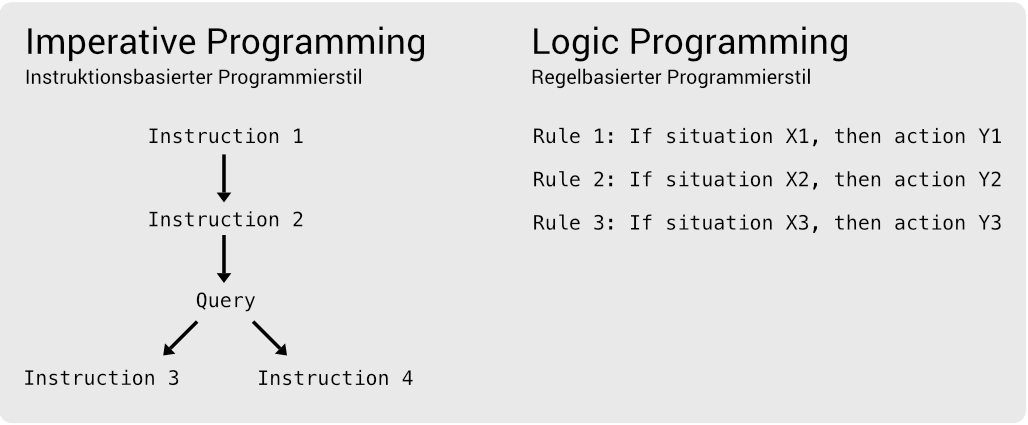
\includegraphics[width=17cm]{chapters/expertensysteme/imperative_vs_rule_based}
    \caption{Imperativer Programmierstil vs. Regelbasierter Programmierstil}
    \label{fig:programmierstil}
\end{figure}

\noindent So ein regelbasierter Ansatz hat vier wichtige Eigenschaften, die den einzelnen Komponenten des Systems zu Gute kommen. Eine Aneinanderreihung von WENN-DANN-Regeln ist\\

\begin{itemize}
    \item \textbf{Modular:} Das Wissen wird unabhängig voneinander in kleineren Regeln dargestellt.
    \item \textbf{Incrementable:} Aufgrund ihrer Modularität, können neue Regeln problemlos hinzugefügt werden.
    \item \textbf{Modifiable:} Das Ändern einer Regel beeinflusst nicht die restlichen Regeln.
    \item \textbf{Transparent:} Regeln können verwendet werden, um das Programmverhalten zu erklären.
\end{itemize}

%------------------------------- Aufbau eines Expertensystems --------------------------------
%---------------------------------------------------------------------------------------------
\subsection{Aufbau eines regelbasierten Expertensystems}
\noindent Regelbasierte Expertensysteme bestehen aus vier verschiedenen Komponenten:\\

\noindent {\fontfamily{pag}\selectfont {\small \textbf{Knowledge Base:}}}\\
Die Wissensbasis enthält das ganze Fachwissen der Experten.\\
Die ganzen WENN-DANN-Regeln sind hier gespeichert.\\

\noindent {\fontfamily{pag}\selectfont {\small \textbf{Inference Engine:}}}\\
Der Regelinterpreter bzw. der Logikkern des ganzen Systems. Mit Hilfe der Regeln aus der Knowledge Base, wird hier das Problem interpretiert, verarbeitet und gelöst.\\

\noindent {\fontfamily{pag}\selectfont {\small \textbf{Working Storage:}}}\\
Hier werden relevante Daten zur aktuellen Problemlösung zwischen gespeichert.\\

\noindent {\fontfamily{pag}\selectfont {\small \textbf{User Interface:}}}\\
Die Schnittstelle zwischen dem Benutzer und der Inference Engine.\\

\noindent Der Working Storage, die Benutzerschnittstelle sowie die Inference Engine bilden die Hülle des Systems. Die Knowledge Base soll theoretisch austauschbar sein, jedoch ist dies in der Praxis nur sehr schwer umsetzbar, denn die Inference Engine ist zu sehr auf das Wissen der Knowledge Base zugeschnitten.

\begin{figure}[H]
    \centering
    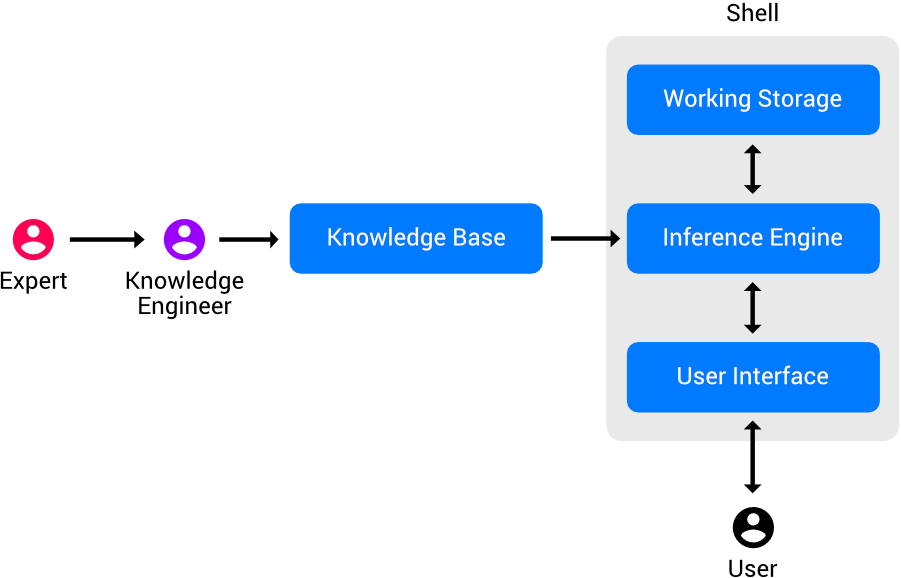
\includegraphics[width=17cm]{chapters/expertensysteme/aufbau_expertensystem}
    \caption{Aufbau eines regelbasierten Expertensystems}
    \label{fig:aufbau}
\end{figure}

%------------------------------- Wie wird Wissen abgearbeitet? --------------------------------
%----------------------------------------------------------------------------------------------
\subsection{Wie wird Wissen abgearbeitet?}
\noindent Die Inferenz der Regeln erfolgt intern über Goal Trees, auch AND-OR-Trees genannt. Ein Goal Tree weist die üblichen Baumeigenschaften auf. Das Topgoal ist die Wurzel des Baumes, dementsprechend sind die Subgoals die Teilbäume des Baumes, welche selbst wiederum Goal Trees sind. Es gibt zwei Arten von Knoten:\\

\noindent \textbf{AND-Knoten:} Hier müssen alle Teilbäume erfüllt werden.\\
\textbf{OR-Knoten:} Ein Teilbaum muss erfüllt werden.\\

\noindent Es gibt generell zwei verschiedene Ansätze um die Problemstellung zu lösen, entweder anhand des \textbf{Forward Chainings} oder seinem Gegenstück, anhand des \textbf{Backward Chainings}.



%----------------------------------------------------------------------------------------
%	Forward Chaining
%----------------------------------------------------------------------------------------
\section{Forward Chaining}
\noindent Das Forward Chaining wird auch \textbf{Data Driven Reasoning} genannt, denn man fängt mit einer gegebenen Faktenbasis \textit{(den Basiszuständen)} an. Dies sind die Blätter des Goal Trees. Von hier aus schließt man mit Hilfe der Regeln aus der Knowledge Base neue Fakten und tastet sich immer weiter vor bis man schlussendlich aus den geschlossenen Fakten eine Diagnose tätigen kann. Dies ist unser Topgoal, also die Wurzel des Goal Trees.\\

\noindent Zum Veranschaulichen ein kleines Beispiel aus der Tierwelt:\\
In der freien Natur sehen wir ein Tier, was wir identifizieren wollen. Um nun unser Problem zu lösen benutzen wir ein Expertensystem, welches mit der Methode des Forward Chaining arbeitet.
Wie oben bereits schon erwähnt fangen wir beim Forward Chaining mit einer Faktenbasis an. Auf unser Problem bezogen bedeutet dies, dass wir Beobachtungen aufstellen müssen. Zum Beispiel sehen wir, dass einige Tiere Federn haben, andere wiederum einen Schnabel. Einige leben in der Kälte, andere sind nachtaktiv. Mit Hilfe dieser Basiszustände versucht das System eine Lösung zu inferieren.\\

\begin{figure}[H]
    \centering
    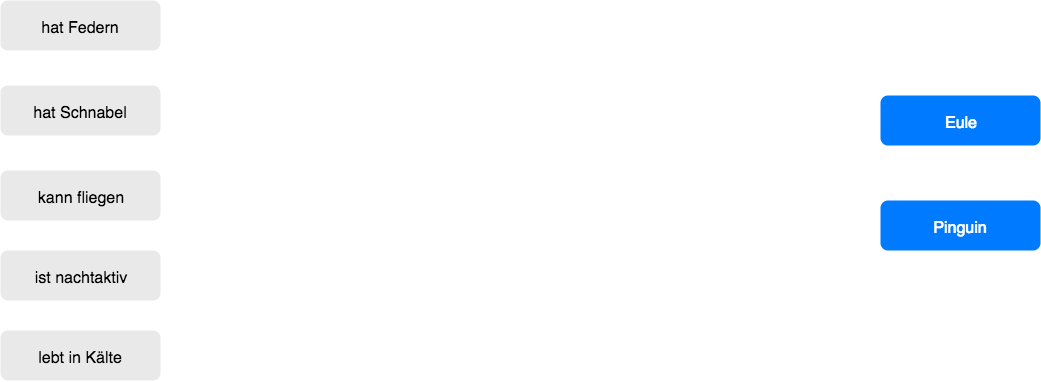
\includegraphics[width=17cm]{chapters/expertensysteme/forward_chaining/forward_chaining_1}
    \caption{Beginnen mit unserer Faktenbasis, hier links}
    \label{fig:forward_chaining_1}
\end{figure}

\noindent Mit den Regeln aus der Knowledge Base kann das System nun schrittweise zu Teillösungen voranschreiten. Die erste Regel könnte lauten: \textbf{WENN} Federn und \textbf{WENN} Schnabel, \textbf{DANN} Vogel.
\begin{figure}[H]
    \centering
    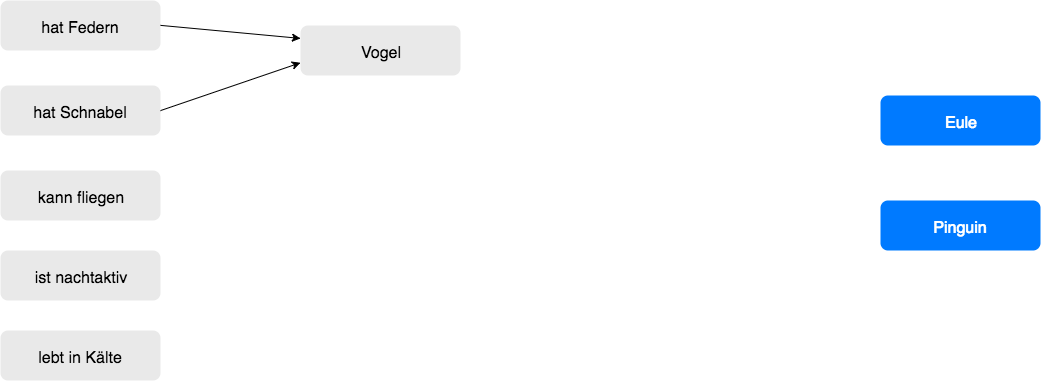
\includegraphics[width=17cm]{chapters/expertensysteme/forward_chaining/forward_chaining_2}
    \caption{Neue Teillösungen inferieren}
    \label{fig:forward_chaining_2}
\end{figure}

\noindent Eine andere Regel könnte lauten: \textbf{WENN} Vogel und \textbf{WENN} fliegen, \textbf{DANN} flugfähiger Vogel.
\begin{figure}[H]
    \centering
    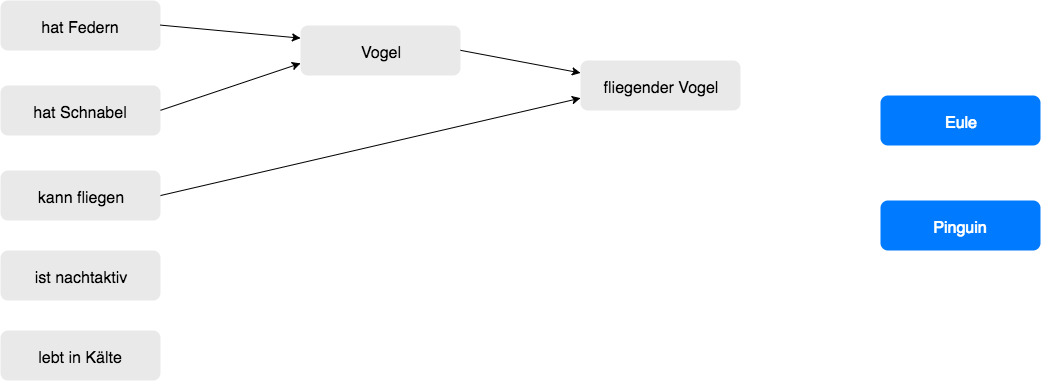
\includegraphics[width=17cm]{chapters/expertensysteme/forward_chaining/forward_chaining_3}
    \caption{Weitere Teillösung inferieren}
    \label{fig:forward_chaining_3}
\end{figure}

\clearpage
\noindent Eine weitere Regel könnte lauten: \textbf{WENN} fliegender Vogel und \textbf{WENN} nachtaktiv, \textbf{DANN} Eule. Somit hat unser Expertensystem von unseren anfänglichen Beobachtungen geschlussfolgert, dass es sich um eine Eule handeln muss.
\begin{figure}[H]
    \centering
    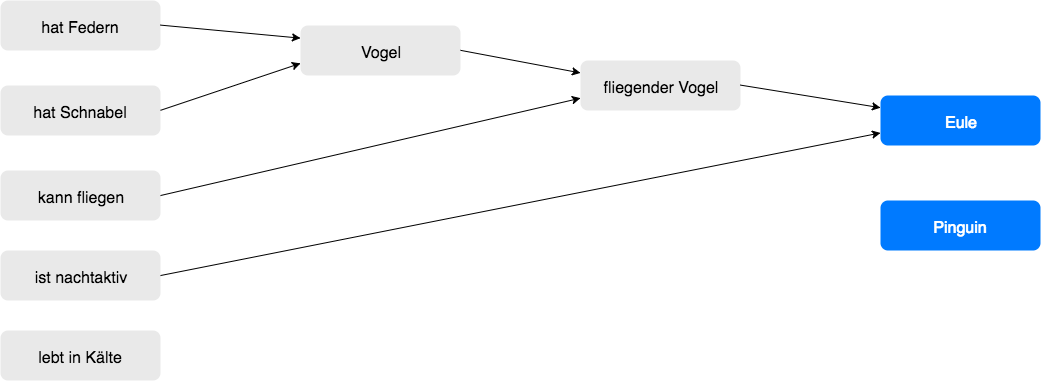
\includegraphics[width=17cm]{chapters/expertensysteme/forward_chaining/forward_chaining_4}
    \caption{Topgoal erreicht}
    \label{fig:forward_chaining_4}
\end{figure}

\noindent Würden wir nun ein weiteres Tier sehen und wieder unser Expertensystem fragen, könnte das ganze so aussehen:
\begin{figure}[H]
    \centering
    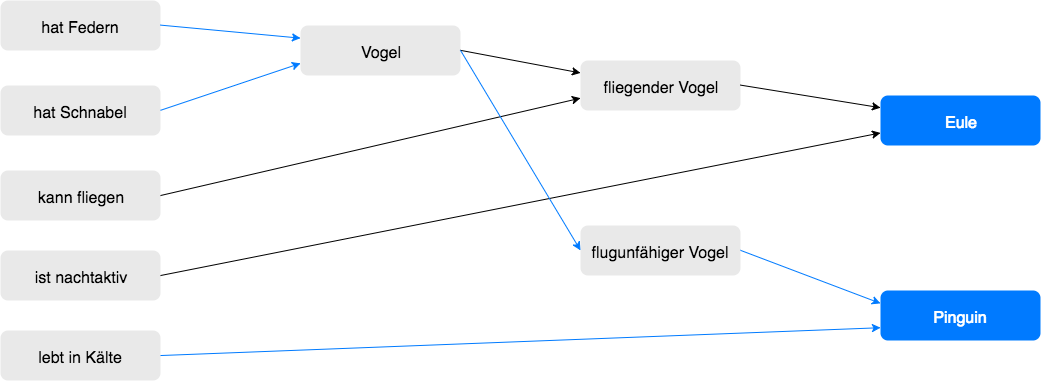
\includegraphics[width=17cm]{chapters/expertensysteme/forward_chaining/forward_chaining_5}
    \caption{Von unserer Faktenbasis inferiert das System, dass es sich um einen Pinguion handelt.}
    \label{fig:forward_chaining_5}
\end{figure}

\noindent Das Forward Chaining ist anwendbar auf Probleme mit nicht aufzählbaren Lösungen. In der Realität wird Forward Chaining daher in Design- und Konfigurationssysteme genutzt.



%----------------------------------------------------------------------------------------
%	Backward Chaining
%----------------------------------------------------------------------------------------
\section{Backward Chaining}
Backward Chaining ist wie vorher schon erwähnt das Gegenstück zum Forward Chaining. Hier beginnt man beim Topgoal und zerlegt dieses in die ursprünglichen Subgoals. Da die Subgoals prinzipiell wieder Topgoals sind zerlegt man diese auch wieder in Subgoal. Dies macht man solange bis man wieder bei den Blättern, also den Fakten angelangt ist. Man kann dazu auch sagen: Das System inferiert von den Hauptlösung zur Teillösung. Diese Teillösungen werden dabei im Working Storage gespeichert. Nun wird dies wieder an unserem bekannten Beispiel mit Eule und Pinguin illustriert.

\subsection*{Beispiel}
\begin{figure}[H]
    \centering
    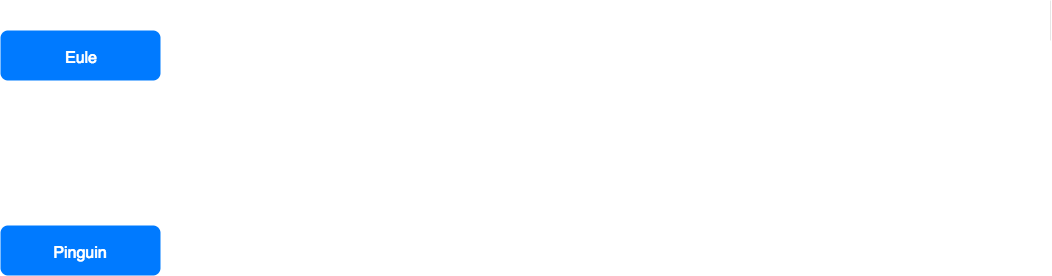
\includegraphics[width=17cm]{chapters/expertensysteme/backward_chaining/backward_chaining_1}
    \label{fig:backward_chaining_1}
\end{figure}

Wir haben nun die beiden Topgoals Eule und Pinguin gegeben. Nun möchten wir wieder zu den Teillösungen gelangen. Dies geschieht wie auch beim Forward Chaining mit den Wenn-Dann Regeln. In diesem Beispiel wäre die erste Regel:

Wenn Eule, dann kann fliegen und ist nachtaktiv

\begin{figure}[H]
    \centering
    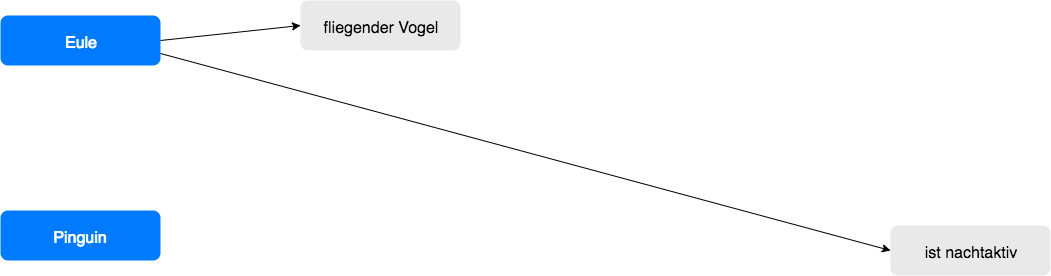
\includegraphics[width=17cm]{chapters/expertensysteme/backward_chaining/backward_chaining_2}
    \label{fig:backward_chaining_2}
\end{figure}

Dies macht man nun solange bis man wieder bei der Faktenbasis ist.

\begin{figure}[H]
    \centering
    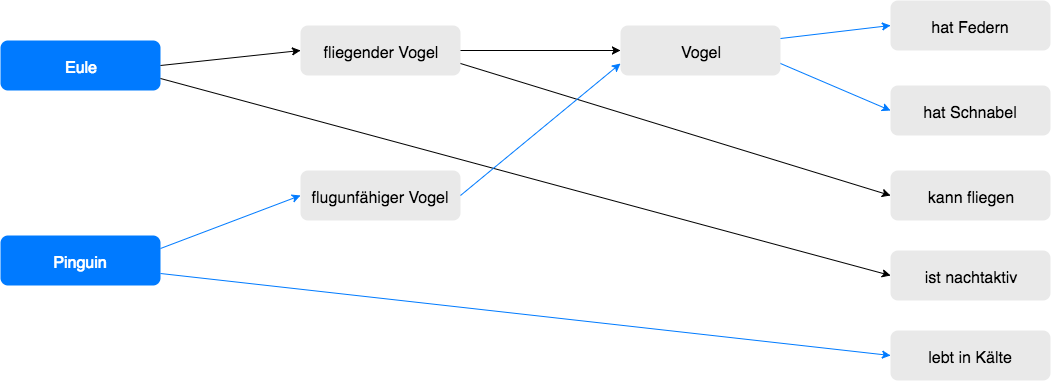
\includegraphics[width=17cm]{chapters/expertensysteme/backward_chaining/backward_chaining_3}
    \label{fig:backward_chaining_3}
\end{figure}

\noindent Diese Art von regelbasierten Expertensystem ist anwendbar auf Probleme mit strukturierter Selektion und auf Probleme, die aufzählbare Lösungen haben. Hier könnte sich die Frage stellen: Warum nur auf Probleme mit aufzählbaren Lösungen? Diese Frage beantwortet sich fast schon von allein, da jede Lösung mindestens eine Regel haben muss.

\noindent In der Realität wird Backward Chaining daher in Identifaktions- und Diagnosesysteme zum Einsatz.


%----------------------------------------------------------------------------------------
%	Umgang mit Unsicherheit
%----------------------------------------------------------------------------------------
\section{Umgang mit Unsicherheit}
Im regelbasierten Expertensystem gibt es nur absolute Angaben, also nur richtig oder falsch. Dies ist aber nicht Realitätsnah, da Benutzer nicht immer absolut sicher sind. Außerdem kann es auch sehr gut sein, dass Unsicherheiten in den Regeln vorkommen. Durch all diese Unsicherheiten gibt es das Bedürfnis mit diesen Unsicherheiten umzugehen. 

Eine Möglichkeit mit den Unsicherheiten sind die Certainty Factors (CF) zu deutsch Sicherheitsfaktoren.

\subsection{Certainty Factors}
Die CF's liegen zwischen -1 und 1. Dabei entspricht -1 falsch, 1 wahr und 0 kompletter Unwissenheit. Den CF des Topgoals kann man berechnen, in dem man den minimalen CF der Subgoals mit dem CF der abschließenden Regel multipliziert. Dies wird im nächsten Beispiel veranschaulicht. Desweiteren gilt:
\begin{itemize}
	\item ist ein Subgoal mit -1 bewertet, so ist das Topgoal nicht erfüllbar
	\item erhält das Topgoal einen CF mit 1, so ist dieses mit Sicherheit erfüllbar.
\end{itemize}
In manchen Systemen kann es vorkommen, dass die Werte -1 und 1 als sehr mächtig interpretiert werden und man noch andere Werte zu lassen möchte. Daher kann man sich eigene Schwellen einrichten, so könnte man Beispielsweise sagen: "`Wir erkennen schon einen Wert ab 0.75 als wahr an und einen -0.75 als falsch."' Aber auch dies ist immer System und Benutzer abhängig. 

\subsection*{Beispiel}
Betrachten wir nun die Regel:

{\bfseries Wenn flugunfähiger Vogel und lebt in Kälte dann Pinguin.}

\begin{itemize}
\item {\bfseries flugunfähiger Vogel} ist ein Subgoal welches durch alle Regeln und Subgoals, die zu ihm führen mit einem CF=0.4 bewertet wurde.
\item {\bfseries lebt in Kälte} ist ein Fakt, welcher einen CF=-0.3 erhalten hat. Dieser wurde vom Benutzer eingegeben. 
\item Die {\bfseries Wenn-Dann-Regel} ist eine sehr sichere Regel die mit 0.9 bewertet wurde. Man könnte sich noch vorstellen, dass der flugunfähige Vogel in der Kälte eine Möwe mit gebrochenen Flügel ist, aber das ist auch schon alles.
\end{itemize}

Der minimale Wert der Subgoals ist hier -0.3.

$\Rightarrow$ CF für Pinguin $-0.3 \cdot 0.9 = -0.27$

Die -0.27 sagen uns nun das wir eher nicht wissen, dass es ein Pinguin ist, aber wir schon sehr unsicher sind ob es wirklich kein Pinguin ist.



Es kann vorkommen, dass es in einem regelbasierten Expertensystem mehrere Wege gibt, um auf das gleiche Ziel zu gelangen. Wenn dieser Fall eintritt möchte man die CF's, die durch die verschiedenen Regeln für das gleiche Topgoal entstehen in irgendeiner Form kombinieren können. Dazu gibt es verschiedene Möglichkeiten. Eine dieser Möglichkeiten ist unter anderem MYCINs Certainty Algebra.


\subsection{MYCINs Certainty Algebra}
Als Voraussetzung für diese Algebra muss man mindestens $2$ CF's haben, die man kombinieren möchte, also X und Y. 
Hat man dies gegeben, so kann man den kombinierten CF mit Hilfe der folgenden Algebra berechnen:

	$$
	CF(X,Y) = 
	\begin{cases}
		X+Y \left(1-X\right) 
		  & X \ge 0 \wedge Y \ge 0 \\
		\left( X+Y\right)
		/ \left(1-min \left(|X|, |Y|\right)\right) &  X < 0 \vee Y < 0 \\
		X+Y \left(1+X\right)  & X < 0 \wedge Y < 0
	\end{cases}
	$$

Wenn man mehr als 2 CF's gegeben hat, dann kombiniert man 2 und das Ergebnis dann mit den weiteren 

z.B.: a, b, c kombiniere erst d=CF(b,c) erg=CF(a,d)

$\Rightarrow$ Die Reihenfolge spielt hier also keine Rolle.



\subsection*{Beispiel zur Kombination von CF's mithilfe von MYCINs Certainty Algebra}
Regeln:
\begin{itemize}
		\item[1.] flugunfähiger Vogel, isst Fisch, lebt auch in der Antarktis $\Rightarrow$ Pinguin CF=0.51
		\item[2.] flugunfähiger Vogel, ist schwarz/weiß, kann schwimmen $\Rightarrow$ Pinguin CF=-0.3
			\item[3.]  Vogel, isst Fisch, kann schwimmen, lebt auch in der Antarktis $\Rightarrow$ Pinguin CF=0.4
\end{itemize} 
Nun haben wir den Fall, dass wir 3 Regeln haben, die man kombinieren möchte.
Zuerst sei X=0.51 und Y=-0.3, also haben wir den Fall, dass einer der Werte unter 0 ist und der andere über 0. Daher müssen wir $CF \left( X,Y \right) =\left( X+Y\right) / \left(1-min \left(|X|, |Y|\right) \right)$ anwenden. Also:


$CF \left( 0.51,-0.3 \right) =\left( 0.51-0.3 \right) / \left(1-min \left(|0.51|, |-0.3|\right) \right)$ \\
Das ergibt 0.3. 
Nun muss noch die 0.3 mit der 0.4 kombiniert werden. Wenn man dies macht kommt ein Wert von 0.58.



%----------------------------------------------------------------------------------------
%	Verhalten erklören
%----------------------------------------------------------------------------------------
\section{Verhalten erklären}
\noindent Expertensysteme können ihr Verhalten dem Nutzer erklären, sollte dieser eine simple Nachfrage stellen. Hierbei wird zwischen zwei Arten von Fragen unterschieden.

\subsection{Why-Questions}
\noindent Why-Questions sind Fragen die angeben, warum die genau diese Anfrage dem Nutzer gestellt wurde. In einem Goal Tree muss sich das System nur eine Ebene nach oben bewegen um die Antwort auf die gestellte Frage zu finden.\\

\noindent {\fontfamily{pag}\selectfont {\small \textbf{Beispielaufruf:}}}\\
\noindent \textbf{System:} Ist fliegender Vogel?\\
\textbf{User:} why?\\
\textbf{System:} Eule $\Leftarrow$ fliegender Vogel, ist nachtaktiv

\subsection{How-Questions}
\noindent How-Questions beantworten warum diese spezifische Lösung inferiert wurde. Das Expertensystem hat sich seinen Arbeitsweg abgespeichert und ruft diesen Schritt für Schritt ab, falls der Nutzer Fragen stellt.\\

\noindent {\fontfamily{pag}\selectfont {\small \textbf{Beispielaufruf:}}}\\
\noindent \textbf{System:} Tier ist Eule.\\
\textbf{User:} how Eule?\\
\textbf{System:} fliegender Vogel, ist nachtaktiv $\Rightarrow$ Eule\\
\textbf{User:} how fliegender Vogel?\\
\textbf{System:} Vogel, kann fliegen $\Rightarrow$ fliegender Vogel


%----------------------------------------------------------------------------------------
%	Zusammenfassung
%----------------------------------------------------------------------------------------
\section{Zusammenfassung}
Expertensysteme simulieren menschliche Experten, die nur aus WENN-DANN-Regeln bestehen. Die Lösungen, die die Expertensysteme generieren sind basiert auf Regeln, die von der Problemstellung vorgegeben werden. Es kann mit Unsicherheiten umgehen, sei es Unsicherheiten in den Regeln oder auch von der Benutzereingabe her. Das Programm kann sich selbst erklären solange die Fragen How bzw. Why basiert sind.

\begin{table}[H]
    \centering
    \label{zsmfassung_Chaining}
    \begin{tabular}{c|c|c}
                                    &\textbf{Forward Chaining}                  &\textbf{Backward Chaining}         \\\hline
        \textbf{Ansatz}             & Data Driven Reasoning                     & Goal Driven Reasoning             \\\hline
        \textbf{Goal Tree}          & von Blättern aufgebaut                    & von Wurzel aufgebaut              \\\hline
        \textbf{Lösungen finden}    & Lösungszustände durch Regeln akzeptiert   & Jede Lösung (mind.) ein Topgoal   \\\hline
        \textbf{Anwendung}          & nicht aufzählbare Lösungsmenge            & aufzählbare Lösungsmenge          \\
    \end{tabular}
\end{table}



%----------------------------------------------------------------------------------------
%	Kritikpunkte
%----------------------------------------------------------------------------------------
\section{Kritikpunkte}
Es gibt einige Kritikpunkte an den Expertensystemen, da die Knowledge Base aufwändig zu erstelle ist. Meistens benötigt man einen Experten und zustätzlich noch einen Knowledge Engineer, der das Expertenwissen in eine regelbasierte Computersprache umsetzen kann. Das Wissen des Expertensystems ist kein echtes Wissen, sondern nur regelbasiert, somit kann nur neues Wissen angelegt werden, wenn dieses wieder in die Regelform gebracht wurde. Es gibt zwar die Möglichkeit das System zu hinterfragen mit den How- und Why-Questions, jedoch gibt das System meistens nur die Position im Goal Tree an, aber kein Hintergrundwissen oder Begründungen für den Benutzer.
\chapterimage{chapter_head_1.png}

\chapter{Theorembeweiser}
\section{Einleitung}
Der Eine kennt sie überhaupt nicht, der Andere womöglich noch aus der Schule, aber wirklich
jeder Student mit Mathematikkursen kennt sie - die Beweise.
In der Mathematik werden seit jeher Theorien aufgestellt, bewiesen und mitunter auch widerlegt.
Man kann das Beweisen dieser als eine Art Kunstform ansehen.
So gibt es häufig nicht nur den einen Weg zum Ziel, sondern oftmals auch schnellere, schönere und/oder einfachere.
Allen gemein ist allerdings, dass Außenstehende damit kaum etwas anfangen können. Nichtsdestotrotz resultieren die Bemühungen der Mathematiker nicht zuletzt in einen sichtbaren Nutzen.
Als ein Beispiel sei hierbei das Vier-Farben-Problem genannt. Kurz und knapp geht es um die Frage: \enquote{Ist es möglich eine Landkarte mit lediglich vier verschiedenen Farben so einzufärben, so dass am Ende alle benachbarten Länder verschiedenfarbig sind?}
Die Frage entstand bereits im 19. Jahrhundert, als das Drucken von zusätzlichen Farben noch mit erhöhtem Aufwand einherging. 1852 formulierte Francis Guthrie erstmals dazu einen Satz als Vermutung. Dieser erlangte schnell Popularität und es folgten eine Reihe von Beweisen, welche dann früher oder später widerlegt wurden. Erstmals bewiesen wurde er 1976 von Appel und Haken, welche zu jener Zeit frisch entwickelte Methoden zum computergestützten Beweisen von Theoremen anwendeten. Dazu wurde das Problem zunächst auf die Ebene der Graphentheorie getragen und anschließend mit einer Mischung aus klassischen und computerbasierten Beweisen zu einem positiven Ergebnis gebracht. Das allgemeine Problem wurde dabei auf 1936 Fälle (später 1478) reduziert, welche der Computer dann einzeln durchprüfen konnte. Es gibt vor allem zwei Hauptkritikpunkte an Appel und Hakens Beweis:
\begin{enumerate}
\item Es wurde ein Computer benutzt, sodass nicht alles verifiziert werden kann.
\item  Gerade der Teil, der per Hand geprüft werden müsste, ist so kompliziert und
mühsam, dass ihn, soweit bekannt, niemand unabhängig geprüft hat.
\end{enumerate}
Man wird schnell bemerken, dass dies ein durchaus stark diskutiertes Thema ist. So argumentieren Kritiker, dass Beweise stets von Menschenhand nachprüfbar und nachvollziehbar sein sollten, oder zweifeln gar die Korrektheit der maschinellen Beweise an. Nun, in der Tat verstecken sich häufig Fehler in Computerprogrammen, sodass die verwendeten Algorithmen mitunter inkonsistent arbeiten. 1996 bewiesen N. Robertson, D. P. Sanders, P. Seymour und R. Thomas den Vier-Farben-Satz mit der gleichen Beweisidee, reduzierten allerdings die Anzahl der Problemfälle auf 633. Mittlerweile gibt es noch weitere unabhängige Beweise dazu. Man kann zwar nicht ausschließen, dass der Mensch oder die Maschine in einem geführten Beweis Fehler gemacht haben, aber je häufiger ein Theorem unabhängig bewiesen wird, desto
unwahrscheinlicher wird es, dass all diese Beweise fehlerhaft sind. Anhand der folgenden Tabelle von Thomas C. Hales\cite{hales_formalproof} sieht man, dass es seit längerem Bestrebungen gibt, mathematische Aussagen mit dem Computer zu beweisen.

\begin{table}
\begin{tabular}{ccccc}
\toprule
Jahr & Theorem & Beweissystem & Formaler Beweis & Klassischer Beweis \\ \midrule
1986 & First Incompleteness & Boyer-Moore & Shankar & Gödel \\
1990 & Quadratic Reciprocity & Boyer-Moore & Russinoff & Eisenstein \\
1996 & Fundamental - of Calculus & HOL Light & Harrison & Henstock \\
2000 & Fundamental - of Algebra & Mizar & Milewski & Brynski \\
2000 & Fundamental - of Algebra & Coq & Geuvers et al. & Kneser \\
2004 & Four-Color & Coq & Gonthier & Robertson et al. \\
2004 & Prime Number & Isabelle & Avigad et al. & Selberg-Erdös \\
2005 & Jordan Curve & HOL Light & Hales & Thomassen \\
2005 & Brouwer Fixed Point & HOL Light & Harrison & Kuhn \\
2006 & Flyspeck I & Isabelle & Bauer-Nipkow & Hales \\
2007 & Cauchy Residue & HOL Light & Harrison & classical \\
2008 & Prime Number & HOL Light & Harrison & analytic proof \\
\bottomrule
\end{tabular}
\end{table}

Darüber hinaus haben sich über die Jahre hinweg verschiedene Systeme und auch verschiedene Anforderungen an diese entwickelt.
Im folgenden möchte ich erklären was Theorembeweiser (kurz TB) sind, wie diese arbeiten und wofür wir sie brauchen.
Dazu werden der formale Beweis, Erfüllbarkeitsprobleme (kurz SAT, engl. für \enquote{satisfiability}), interaktive TB und automatisierte TB vorgestellt und zum Schluss gibt es einen Ausblick auf die Anwendungen und zukünftige Bestrebungen.

\section{Der formale Beweis}
Klassische Beweise sind in der Regel so gehalten, dass Mathematiker diese gut
verstehen bzw. nachvollziehen können. Hinter Bezeichnungen und Abkürzungen
verstecken sich dabei häufig sehr spezielle mathematische Ausdrücke in Form von
Eigenschaften und Formeln, welche der Laie ohne Frage als Fremdsprache
identifizieren kann. Darüber hinaus führen Mathematiker Beweise häufig
schemenhaft oder auch anhand von Beispielen, die dann verallgemeinert werden
können. So kommt es nicht selten vor, dass für eine Aussage mehrere Fälle gezeigt
werden müssen, aber nur einer mit dem Zusatz vorgerechnet wird, dass die anderen
Fälle analog behandelt werden. Ebenfalls gern verwendet werden Formulierungen wie
\enquote{Ohne Beschränkung der Allgemeinheit} (kurz OBdA) oder \enquote{trivial}, deren
Bedeutung dem Mathematiker klar ist. Der klassische Beweis erfordert auch häufig
kreative Wege und Beweisideen, die mitunter erst nach einigem Probieren, etwa
Umformen und Umbenennen, ersichtlich werden. Ein formaler Beweis hingegen
umfasst alles. Jede Implikation muss auf ihre Gültigkeit geprüft und jeder logische
Schritt, bis zurück zu den fundamentalen Axiomen der Mathematik, muss vorhanden
sein. Um zum Beispiel zu zeigen, dass ein Graph planar ist, reicht es dem
Mathematiker, wenn der Graph entsprechend gezeichnet werden kann. Im formalen
Beweis würde eine zusammenhängende Argumentationskette entstehen, die den
theoretischen Kontext vollkommen abdeckt. Wie man sich leicht überlegt wird so
etwas leicht unüberschaubar und umfangreich. Um dies ein wenig zu verdeutlichen
möchte ich einen computergefertigten formalen Beweis vorstellen ohne dabei auf den
mathematischen Hintergrund einzugehen.
Als Beispiel sei die Robbins Algebra gewählt. Der Computer hat damals fast 8 Tage gebraucht um diese Lösung zu ermitteln. Brandon Fitelson benutz in seiner Arbeit \enquote{Using Mathematica to Understand the Computer Proof of the Robbins Conjecture}~\cite{robinsconjecture} eine andere Darstellungsform um den Beweis übersichtlicher und nachvollziehbarer zu gestalten.
Er bemerkt, dass es trotzdem an einigen Stellen äußerst schwierig ist, zu verstehen, wie tatsächlich vorgegangen wird.
Interessierten an den mathemathischen Aspekten empfehle ich daher seine Aufarbeitung.
Er nutzt die klassische Notation, in der die Negation in der typischen Boolschen Schreibweise dargestellt wird, wodurch dem Betrachter einige Erleichterungen beim Lesen verschafft werden.
Ich zeige an dieser Stelle den eigentlichen Beweis von W. McCun, welcher mit dem Equational Theorem Prover (kurz EQP, ein automatisierter Theorembeweiser) angefertigt wurde und im Anschluss folgt eine aufgearbeitete Fassung von Thomas C. Hales~\cite{hales_formalproof}, in der übersichtlich zwischen Umformungen, Substitutionen und Anwendungen der Robbins Identität unterschieden wird.

Um beide Notationen in Einklang zu bringen sei gesagt, dass   $n(\ldots)$, $[\dots]$ und $\bar(x)$ die Negation darstellen und die Verknüpfung $(x,y) \rightarrow x + y$ aus dem 1. Teil durch $(x,y) \rightarrow xy$ in Hales Aufarbeitung ersetzt wurde.
Der direkte Vergleich dieser beiden Beweise zeigt eindeutig, dass der
Computerbeweis mitunter sehr schwer zu lesen ist und durchaus unhandlich sein
kann. Heutzutage wird daher immer häufiger auf interaktive Beweise und vor allem
auch eigene Ausgabestrukturen gesetzt, wie z.B. Isar (der Beweissprache von
Isabelle). Nach Möglichkeit sollen diese sowohl der Maschine als auch dem Menschen
ermöglichen, die Sprache gut zu lesen und zu verstehen.
Wir können diesen formalen Beweis nun als das Endergebnis verstehen, welches wir hier sehen, eine Kette von logischen Inferenzschritten.

\section{Korrektheit eines computergefertigten Beweises}
In diesem Abschnitt wird die Fragestellung diskutiert, in welchem Maße man auf die Korrektheit eines computergefertigten formalen Beweises vertrauen kann. Dazu wird zunächst darauf eingegangen, in wie weit menschliches Versagen die Korrektheit eines maschinellen Beweises gefährdet und anschließend wird das Problem abstrahiert, indem allgemeine Aussagen über die Korrektheit eines beliebigen Beweises gemacht werden.\\
Beschäftigt man sich mit der Frage, ob man eher einem computergefertigten Beweis als einem von Hand gefertigten Beweis vertraut, stößt man oft auf den ersten naiven Ansatz, dem Computer zu vertrauen, da diesem erfahrungsgemäß keine Flüchtigkeitsfehler unterlaufen. Dieser Ansatz ist auch durchaus berechtigt, es ist in der Vergangenheit schon oft vorgekommen, dass sich Beweise von viel diskutierten Theoremen erst einige Zeit nach ihrer Veröffentlichung als fehlerhaft herausgestellt haben. Jedoch ist zu beachten, dass auch maschinell erstellte Beweise von menschlichen Fehlern betroffen sein können. Man hat nämlich ebenfalls keine absolute Gewissheit, dass die Algorithmen, welche der Computer zum Beweisen benötigt, fehlerfrei sind, da diese auch vom Menschen geschaffen wurden. Hinzu kommt, dass maschinell erstellte Beweise meistens so kompliziert sind, dass sie nur sehr schwer per Hand nachgeprüft werden können. Also lässt sich zusammengefasst sagen, dass bei maschinell erstellten Beweisen und bei per Hand erstellten Beweisen die Gefahr von menschlichem Versagen besteht, aber die per Hand erstellten Beweise sich leichter überprüfen lassen.\\
Geht man nun davon aus, dass dem Menschen keine Fehler unterlaufen würden, hätte man leider trotzdem keine absolute Gewissheit, dass ein Beweis korrekt ist. Dies besagt der zweite Gödelsche Unvollständigkeitssatz, der besondere Bedeutung in der modernen Logik erlangt hat. Dieser Satz besagt:
\begin{equation*}
Jedes\ hinreichend\ mächtige\ konsistente\ System\ kann\ die\ eigene\ Konsistenz\ nicht\ beweisen.
\end{equation*}
Im Folgenden wird eine stark vereinfachende Erklärung dieses Satzes vorgestellt, welche aber zum Verständnis der Problematik völlig ausreichend ist. Eine detaillierte und präzise Erläuterung wäre Aufgabe einer Vorlesung in mathematischer Logik und Mengenlehre.\\
Der Aufbau eines Beweises ist immer der selbe. Es sind mehrere Voraussetzungen gegeben und aus diesen Voraussetzungen werden so lange logische Schlussfolgerungen gezogen, bis man zu der zu beweisenden Aussage gelangt. Die Korrektheit eines Beweises hängt nun davon ab, ob die Schlussfolgerungen korrekt sind und ob die Voraussetzungen widerspruchsfrei sind. Der zweite Gödelsche Unvollständigkeitssatz besagt nun stark vereinfacht unter anderem, dass man die Widerspruchsfreiheit der Voraussetzungen nicht beweisen kann. Dies lässt sich auch leicht veranschaulichen. Angenommen, man wolle die Widerspruchsfreiheit der Voraussetzungen beweisen. Dazu würde man einen weiteren Beweis benötigen. Dieser hätte aber wieder andere Voraussetzungen, dessen Widerspruchsfreiheit man noch nicht bewiesen hat. Man kann nur die Widerspruchsfreiheit einer Menge von Annahmen zeigen, wenn diese Annahmen widersprüchlich sind. Aus einer widersprüchlichen Annahme lässt sich nämlich jede beliebige falsche Aussage ableiten, dazu gehört auch die Aussage, dass die widersprüchliche Annahme widerspruchsfrei ist.
\paragraph*{}Zusammenfassend lässt sich sagen, dass die allgemeine Korrektheit maschinell erstellter Beweise Raum für verschiedene Meinungen zur Verfügung stellt. Sowohl Beweise per Hand als auch maschinelle Beweise sind nicht vor Fehlern des Menschen geschützt. Fehler bei Beweisen, die vom Menschen erstellt wurden, lassen sich sich leichter entdecken, dafür arbeitet der Computer fehlerfrei, wenn die benötigten Algorithmen korrekt sind. Eine absolute Gewissheit, dass ein Beweis korrekt ist, wird man jedoch nie haben.

\section{SAT / SMT}
Hinter einem Erfüllbarkeitsproblem versteckt sich die Frage, ob es für eine aussagenlogische Formel eine Lösung gibt. Man stelle sich jetzt eine einfache
mathematische Ungleichung vor, wie zum Beispiel $3+7<2 \cdot x$. Auf die Frage ob eine natürliche Zahl x existiert, welche diese Formel erfüllt, werden die meisten im Schlaf
eine Antwort geben können. Solche Formeln müssen natürlich nicht auf die natürlichen Zahlen, ja geschweige denn auf die Mathematik beschränkt sein.
Um eine Maschine anleiten zu können Theorien, bzw. Aussagen auf ihre Gültigkeit hin zu überprüfen oder gar diese zu beweisen, muss zunächst eine Struktur
gefunden werden, auf deren Grundlage der Computer entscheiden kann, wann eine Aussage wahr oder falsch wird, eine Sprache. Ohne zu sehr ins Detail gehen zu
wollen, sei an dieser Stelle gesagt, wir benötigen eine Prädikatenlogik. SAT formalisiert dieses Thema und führt Theorien ein, mithilfe derer wir die Aussagen
logischer Konstruktionen, umformen bzw. Belegungen finden können, um diese zu lösen.
Die \enquote{Satisfiability Modulo Theories}, kurz SMT, erweitert dieses System um die Möglichkeit Formeln und Terme um spezielle theoretische Aussagen zu erweitern.
Dies sind in der Regel Terme, welche dann von dem SMT-Löser selbst gar nicht verarbeitet werden können und dessen Wahrheitsgehalt von einem sogenannten
Theorie-Löser ermittelt werden muss. Bei den automatischen Theorembeweisern werde ich noch einmal darauf zurück kommen.
Zusammenfassend ist SAT also die Theorie von der Lösbarkeit prädikatenlogischer Formeln und Terme und SMT eine Erweiterung dieser, durch theoretischen Kontext zunächst ungebundener Natur. Im TB stellt dieses Thema die Schnittstelle zwischen der Formulierung des Problems und deren Lösung dar.

\section{Theorembeweiser}
Wir unterscheiden vor allem zwei Sorten von Löser, die interaktiven und die automatisierten, wobei die Interaktiven heutzutage ebenfalls Methoden mitbringen, welche selbstständig nach dem nächsten Umformungsschritt suchen können. Der offensichtlichste Unterschied ist, dass die Automatisierten, wie der Name schon sagt, automatisch nach einer Lösung suchen. Das Programm wird mit allen nötigen Informationen gefüttert und den Rest übernimmt die Maschine.

\subsection{Interaktive Theorembeweiser}
Sie werden auch gerne Beweisassistenten genannt, da sie den Rahmen stellen um geordnet Beweise anzufertigen. Auf der einen Seite prüfen sie alle Inferenzschritte, können aber auf der anderen Seite auch eigenständige Lösungen mit einbringen. Ebenfalls hilfreich ist, dass sie dem Anwender aufzeigen an welchen Stellen noch Unklarheiten bestehen und welche Aussagen noch gezeigt werden müssen. Ein Nachteil ist, dass solche Beweiser zumeist ein hohes Maß an Verständnis für das Programm und seine Sprache vorraussetzen. In der Regel nutzen sie Logiken höherer Ordnung (kurz HOL, engl. \enquote{higher order logic}). Als Beispiele für diese Art der Beweiser möchte ich HOL Light, PVS, Coq, Mizar und Isabelle nennen.
Im folgenden sehen wir 2 exemplarische Beweise mit Isabelle. Der Erste wird veranschaulicht, wie mit sogenannten \enquote{apply}-Scripts gearbeitet wird, das Zweite, wie mit Isar eine lesbare Form erreicht wird.
Ursprünglich sollte hier ein eigenes kleines Beispiel in der zweiten Variante ausformuliert und mit allerhand Erklärungen ausgeschmückt werden, allerdings sprengt dies den Rahmen, sodass hier lediglich die Kenntnis von den beiden Varianten ausreichen soll.

\subsubsection*{Variante 1}
Gegeben ist eine Listenstruktur mit zwei Funktionen, app und rev. Die Erste soll zwei Listen miteinander verknüpfen, die Zweite die
Reihenfolge umkehren.
Gezeigt werden soll, dass das doppelte Umkehren (der Reihenfolge der Elemente) einer Liste, die ursprüngliche Liste ergibt.
In \cref{fig:isabelle1} sieht man den Kopf des Beweises, mit den Definitionen des Datentyps dieser Listen und der beiden Funktionen app und rev.

Zunächst beginnen wir mit dem Theorem und arbeiten uns dann mit den Lemmas von unten nach oben, immer dann, wenn zusätzliche Aussagen gezeigt werden müssen.
In |1 in \cref{fig:isabelle2} haben wir Isabelle gesagt, dass eine Induktion über die Liste xs durchgeführt werden soll. In \cref{fig:isabelle3} sieht man die Antwort darauf, die zu erfüllenden zwei Ziele:
\begin{itemize}
\item Induktionsanfang und
\item Induktionsschritt.
\end{itemize}
Ähnlich sieht es bei den Lemmas aus.
In \cref{fig:isabelle4} sieht man, wie Isabelle den Beweis akzeptiert und eine Regel mit Platzhaltern zur Verfügung stellt, welche nun zur
Vereinfachung genutzt werden kann.
Lemma rev\_app wird für beide Goals vom Theorem rev\_rev gebraucht und die anderen beiden Lemmas für die beiden Goals von rev\_app. \enquote{[sim]} steht hier für eine Vereinfachung, d.h. Isabelle darf die Regeln anwenden um Termumformungen durchzuführen, z.B. durch \enquote{apply(simp)}.

\begin{figure}
\centering
\caption{Isabelle Proof 1}
\label{fig:isabelle1}
\includegraphics[width=.3\textwidth]{chapters/theoremprovers/isabelle1.png}
\end{figure}

\begin{figure}
\centering
\caption{Isabelle Proof 2}
\label{fig:isabelle2}
\includegraphics[width=.3\textwidth]{chapters/theoremprovers/isabelle2.png}
\end{figure}

\begin{figure}
\centering
\caption{Isabelle Antworten}
\label{fig:isabelle3}
\includegraphics[width=.15\textwidth]{chapters/theoremprovers/isabelle3.png}
\end{figure}

\begin{figure}
\centering
\caption{Isabelle akzeptierter Beweis}
\label{fig:isabelle4}
\includegraphics[width=.2\textwidth]{chapters/theoremprovers/isabelle4.png}
\end{figure}

\subsubsection*{Variante 2}
In \cref{fig:isabelle5} sieht man ein Beispiel, in dem der Beweis eigenhändig durchgeführt wird. Gezeigt werden soll, das Abbildungen von einer Menge in ihre Potenzmenge niemals surjektiv sein können. Ohne genau zu wissen wie die neuen Begriffe, wie assume, from, have und show anzuwenden sind, kann man den Beweis doch bereits recht leicht lesen.
In \cref{fig:isabelle6} sieht man, wie sich der Beweisstatus in |3 verändert hat, nach der Annahme, dass f surjektiv sei. Es wird ein f festgehalten, das Goal hat sich nicht verändert.
In \cref{fig:isabelle7} sieht man die Ausgabe von Isabelle, bevor das Lemma akzeptiert wird (|4).

\begin{figure}
\centering
\caption{Isabelle Beweis}
\label{fig:isabelle5}
\includegraphics[width=.3\textwidth]{chapters/theoremprovers/isabelle5.png}
\end{figure}

\begin{figure}
\centering
\caption{Isabelle Beweisstatus}
\label{fig:isabelle6}
\includegraphics[width=.15\textwidth]{chapters/theoremprovers/isabelle6.png}
\end{figure}

\begin{figure}
\centering
\caption{Isabelle Status vor Lemma}
\label{fig:isabelle7}
\includegraphics[width=.3\textwidth]{chapters/theoremprovers/isabelle7.png}
\end{figure}

\subsection{Automatisierte Theorembeweiser und DPLL(T)}
Nachdem wir nun die interaktiven Theorembeweiser kennen gelernt haben, schauen
wir uns die automatisierten etwas genauer an.
Wir unterscheiden unter anderem
zwei Methoden bei der automatisierten Beweissuche, den Davis-Putnam-Logeman-Loveland Algorithmus (kurz DPLL, auch DPLL(T) wobei T für Theorie steht) und das
Tableaukalkül (auch Baumkalkül, bzw. engl. Method of analytic tableaux).
Beide Herangehensweisen arbeiten auf einer Prädikatenlogik, allerdings sei das Baumkalkül
nur als weiterer Vertreter mit aufgeführt.
Grundlegend wird bei diesem versucht die
 Gegenaussage zu widerlegen.

\section{Maschinengestützte Beweistechniken}

\subsection{Resolution}
Der Begriff der Resolution bezeichnet ein Verfahren der formalen Logik, mit dem eine logische Formel auf Gültigkeit getestet werden kann. Das Resolutionsverfahren, auch Resolutionskalkül genannt, ist ein Widerlegungsverfahren. Hierbei wird ein logischer Widerspruch aus der Negation einer Formel abgeleitet, statt die Allgemeingültigkeit der Formel auf direktem Wege zu zeigen.\\
Diese Ableitung erfolgt mithilfe eines Algorithmus auf rein formalem Weg und kann aus diesem Grund von einem Computerprgramm durchgeführt werden.\\

\subsection{Termersetzungssysteme}
Termersetzungssysteme (TES) sind ein formales Berechnungsmodell in der Theoretischen Informatik. Sie bilden insbesondere die Grundlage der logischen und funktionalen Programmierung. Weiterhin spielen sie eine wichtige Rolle beim Wortproblem und der Terminierungsanalyse.\\
Termersetzungssysteme sind Mengen von so genannten Termersetzungsregeln. Diese Mengen kann man sich wie Gleichungssysteme von Termen vorstellen, bei denen die Gleichung nur von links nach rechts angewendet werden dürfen.\\
Termersetzungssystem sind turing-vollständig, deren Berechnungsstärke ist also in etwa auf einem Level mit anderen Formalismen wie etwa dem Lambda-Kalkül oder den Turingmaschinen.

\subsection{Modellprüfung}
Modellprüfung(engl. Model Checking) ist ein Methode zur vollautomatischen Verifikation einer Systembeschreibung(Modell) gegen eine Spezifikation(Formel). Der Begriff ist abgeleitet von der mathematischen Formulierung des Problems: Für eine gegebene Systembeschreibung M und eine gegebene logische Eigenschaft $\Phi$, prüfe, ob M Modell für $\Phi$ ist (formal M $\models$  $\Phi$).\\
Model Checking wird als ein vollautomatisches Verfahren bezeichnet, da es bei der Durchführung keine Benutzerinteraktion nötig ist, anders als etwa beim interaktiven Theorembeweisen. Die Systembeschreibung wird in einer formalen Sprache erstellt, etwa mit einem Programm, einem endlichen Automaten oder einem Transitionssystem. Die Spezifikation ist eine formale Eigenschaft des Systems, die nachzuweisen ist.\\
Will man nun eine Spezifikation für ein System nachweisen, so gibt man diese in einen Modellprüfer ein und dieser stoppt und gibt ein Korrektheitszertifikat aus, falls die Systembeschreibung die Spezifikation erfüllt. Andernfalls gibt  der model checker ein Gegenbeispiel aus, das eine Verletzung der Verifikation nachweist.

\subsection{Induktion}
Die vollständige Induktion ist, wie aus Mathevorlesungen bekannt, eine Bewismethode, bei der eine Aussage für alle natürlichen Zahlen, die größer als ein Startwert sind, gezeigt wird.\\
Ein Induktionsbeweis wird in zwei Phasen durchgeführt. Zuerst erfolgt der Induktionsanfang, bei dem die Aussage für eine kleinste Zahl gezeigtn wird, um sie dann im Induktionsschritt für eine variable Zahl n für die nächste Zahl n+1 logisch abzuleiten.\\
Dieses Verfahren ist von grundlegender Bedeutung für alle Gebiete der Mathematik und somit auch für maschinengestütztes Beweisen, bei dem man dem Computer die formale Aussage übergibt und sie von diesem durchgeführt wird, wobei hierfür meist einige Hilffsätze vom Computer benötigt werden, die man ihm ebenfalls übergibt.

\subsection{Binäre Entscheidungsdiagramme}
Ein Binäres Entscheidungsdiagramm(BED; engl. binary decision diagram, BDD) ist eine Datenstruktur zur Repräsentaion Boolescher Funktionen. Diese Diagramme werden hauptsächlich im Bereich der Hardwaresynthese und -verifikation eingesetzt.\\
Ein BED ist ein Graph mit den Variablen der Funktion als Knoten und den Entscheidungsmöglichkeiten \emph{Wahr} oder \emph{Falsch} als gerichtete Kanten. So kann man die Variablenbelegungen einer Funktion durchgehen und schauen, welche den Wert \emph{wahr} beziehungsweise den Wert \emph{falsch} haben.\\
Solche Diagramme können dann von einem Computer genutzt werden, um zwei Funktionen auf Gleichheit zu überprüfen oder zu testen, ob es eine Variablenbelegung einer Funktion mit dem Funktionswert \emph{wahr} gibt, also, ob die Funktion erfüllbar ist.

\section{Schlusswort}
Nachdem wir nun einen Einblick in der Welt der TB erhalten haben und in Grundzügen wissen was TB sind und wie sie arbeiten, sollen folgend einige Anwendungen vorgestellt werden.
Da Computerprogramme in verschiedenen Sprachen geschrieben werden, welche ein Vokabular, eine Grammatik und eine Syntax haben, können diese genauso für den theoretischen Inhalt herhalten, wie mathematische Probleme.
Ein Beispiel dafür ist der Beweis des Vier-Farben-Satzes von Neil Robertson, Daniel P. Sanders, Paul Seymour und Robin Thomas, welcher genau genommen zwei Beweise beinhaltet.
Der erste zeigt, dass der benutzte Algorithmus richtig arbeitet, also verifiziert die Korrektheit und der zweite, dass das Theorem gilt.
In der Wirtschaft setzt man Theorembeweiser vor allem für die Verifikation von integrierten Schaltkreisen und Prozessoren ein, z.~B. um kritische Operationen zu prüfen.
Allerdings finden sie auch in fachübergreifenden Gebieten ihren Nutzen. Insgesamt scheinen sie bei der Programmverifikation einer zunehmenden Beliebtheit zu unterliegen.
Der seL4 Mikrokernel, welcher in unzähligen Mobilgeräten vorkommt, wurde zum Beispiel mithilfe von Isabelle geprüft und seine Korrektheit nachgewiesen.
In der Mathematik sind sie noch sehr umstritten und auch wenn die vorhandenen Beweiser mächtige Werkzeuge sind, so können sie ihren menschlichen Kollegen heute noch nicht das Wasser reichen.
Eine naheliegende Anwendung diesbezüglich wäre nämlich das Erschaffen von neuen Theoremen und dabei bringen sie höchstens triviale Aussagen zustande.
Mit \enquote{Automated Theorem Discovery}~\cite{Gao2014} richtet man den Blick auf das Schaffen von neuem Wissen, was allerdings noch in den Kinderschuhen steckt.
Das sogenannte \enquote{Theory-Exploration} hingegen versucht Möglichkeiten zu verwirklichen, um dem Anwender von interaktiven TB, im Falle des Feststeckens, mit Lemmas und Ideen weiter zu helfen.
Man bedenke, heutige TB zeigen nur, was noch nicht bewiesen ist und nicht, wie man solches zeigen kann.
Als Fazit kann man sagen, dass mit dieser Arbeit die Themengebiete gerade einmal angekratzt werden konnte, denn es gibt noch mehr als genug Ungesagtes zu den Theorembeweisern.
Mir persönlich hat die Arbeit von Thomas C. Hales über den Formalen Beweis sehr gut gefallen, da sie zeitgleich einen guten Überblick verschafft.
Ich hatte darüber hinaus ein großes Interesse daran Isabelle einmal kennenzulernen und einen interaktiven TB selbst auszuprobieren.
Auch wenn die Zeit nicht gereicht hat um elegante Beweise zu führen, so konnte man doch zumindest einen Eindruck gewinnen.
Der Internetauftritt von Isabelle~\cite{isabellewebpage} bietet diesbezüglich gut verständliche Tutorials an, die für Interessierte in jedem Fall empfehlenswert sind.

\chapterimage{chapter_head_1.png}

\chapter{Bayessche Netze}

\section{Intro}
Ein Bayessches Netz stellt die Wahrscheinlichkeiten von Ereignissen und deren Abhängigkeit (bzw. Unabhängigkeit) zueinander dar.

Bayessche Netze finden immer dort Anwendungsmöglichkeit, wo Logik und Unwissenheit aufeinandertreffen.
Sie dienen der Vereinfachung von komplexen Problemen mit Hilfe weniger stochastischer Regeln.

In der Praxis finden Bayessche Netze beispielsweise in der Spracherkennung, medizinischen Diagnose, Filtern von Spam, Bildverarbeitung, Analyse von Kaufverhalten und in vielen anderen Gebieten Anwendung.

\begin{figure}[h]
    \centering
    \includegraphics[width=.4\textwidth]{chapters/bayes/bayes_intro.pdf}
    \caption{Beispiel eines Bayesschen Netzes zur Diagnose von Krankheiten (ohne Wahrscheinlichkeiten)}
\end{figure}

\section{Grundlagen der Wahrscheinlichkeitsrechnung}
Einem Ereignis A weisen wir eine Wahrscheinlichkeit p(A) zwischen 0 (tritt nie ein) und 1 (tritt immer ein) zu.

Als marginal probability bezeichnen wir eine Wahrscheinlichkeit p(A), welche keine Abhängigkeiten aufweist.
Beispiel: A = Eine aus einem Skatdeck gezogene Karte ist Kreuz.
p(A) = 1/4 (oder 25~\%)

Als joint probability bezeichnen wir Wahrscheinlichkeiten, welche nebeneinander auftreten. p(A,B)
Beispiel: A (von oben) und B: Die Karte ist ein Bube

Da A und B voneinander unabhängige Ereignisse sind folgt:
p(A,B) = p(A) $\cdot$ p(B) = 1/8 $\cdot$ 1/4 = 1/32

Sind Ereignisse jedoch nicht unabhängig, so müssen wir die Wahrscheinlichkeit von p(A,B) bereits bestimmt haben.
Möchten wir nun für eine große Anzahl Ereignisse Wahrscheinlichkeiten berechnen, so benötigen wir extrem viele Daten.

\begin{center}
\begin{tabular}{ ccccc } \toprule
Sonne scheint & Werktag & Stau & Rasensprinkler & Tage im Jahr \\ \midrule
F & F & F & F & 4 \\
F & F & F & T & 5 \\
F & F & T & F & 2 \\
F & F & T & T & 1 \\
F & T & F & F & 13 \\
F & T & F & T & 2 \\
F & T & T & F & 66 \\
F & T & T & T & ... \\
T & F & F & F & ... \\
T & F & F & T & \\
T & F & T & F & \\
T & F & T & T & \\
T & T & F & F & \\
T & T & F & T & \\
T & T & T & F & \\
T & T & T & T & Errechenbar \\
\bottomrule
\end{tabular}
\end{center}


Bis auf 1 errechenbares Ergebnis benötigen wir die direkten Werte aller Kombinationen.
Wir benötigen also Für N Ereignisse $2^N-1$ Datensätze.
Gerade in der Medizin aus dem Anfangsbeispiel gibt es aber oft extrem viele Ereignisse.

Oftmals ist vieles davon aber auch nicht interessant, bzw. ableitbar.
Die Wahrscheinlichkeit, dass die Sonne scheint ist beispielsweise unabhängig davon ob der Tag ein Werktag ist.

Um die benötigten Datensätze möglichst gering zu halten betrachtet man bedingte Wahrscheinlichkeiten (conditional probability).

\section{Bedingte Wahrscheinlichkeit}
Bedingte Wahrscheinlichkeiten beruhen auf Annahmen.
Man nimmt etwa an, dass die Sonne keinen Einfluss auf die Frage hat, ob es nun ein Werktag ist, sehr wohl jedoch auf die Frage, ob der Sprinkler angeschaltet ist.
Gehen wir weiterhin davon aus, dass an sonnigen Tagen mehr Staus zustande kommen, da z.B. Fahrer geblendet werden.
Zudem gehen wir davon aus, dass werktags mehr Staus auftreten.
Fügen wir zudem noch das Verpassen des Essens hinzu, welches lediglich vom Stau abhängt.

\begin{figure}[h]
    \centering
    \includegraphics[width=.2\textwidth]{chapters/bayes/bayes_example.pdf}
\end{figure}

Unsere benötigten Datensätze mit fiktivem Inhalt:\\
$p(Sonne) = 0,8$\\
$p(Werktag)= 0,7$\\
$p(Rasensprinkler | Sonne) = 0,95$\\
$p(Rasensprinkler | !Sonne) = 0,20$\\
$p(Stau | Sonne,Werktag) = 0,8$\\
$p(Stau | !Sonne, Werktag) = 0,75$\\
$p(Stau | Sonne, !Werktag) = 0,15$\\
$p(Stau | !Sonne, !Werktag) = 0,05$\\
$p(Essen verpasst | Stau) = 0,5$\\
$p(Essen verpasst | !Stau) = 0,05$\\

Von 31 Datensätzen in einer Tabelle mit joint probabilities haben wir nun nur noch 10 benötigt Wahrscheinlichkeiten und können alle anderen nun problemlos errechnen. (Beispiel folgt)

Um bedingte Wahrscheinlichkeiten effektiv nutzen zu können benötigen wir einige Definitionen:
\begin{equation*}
p(A,B) = p (A | B) \cdot p (B)
\end{equation*}
Daraus folgt direkt:
\begin{equation*}
p(A,B,C) = p(A | B,C) \cdot p(B,C) = p(A | B,C) \cdot p(B | C) \cdot p(C)
\end{equation*}
Dies lässt sich für N Ereignisse wie folgt darstellen (Chain Rule):
\begin{equation*}
P\left(\bigcap_{k=1}^N A_k\right)  = \prod_{k=1}^N  \mathrm P\left(A_k \,\Bigg|\, \bigcap_{j=1}^{k-1} A_j\right)
\end{equation*}
Zudem bezeichnen wir A als von B unabhängig, wenn gilt:
\begin{equation*}
p(A | B) = p(A)
\end{equation*}
und A als von B unabhängig unter der Prämisse C, wenn gilt:
\begin{equation*}
p(A | C) \cdot p(B | C) = p(A,B | C)
\end{equation*}
%
Mit Hilfe der Chain-Rule können wir nun für das Beispiel von oben jede mögliche joint probability ausrechnen.
%
\subsection{Rechenbeispiel}
Wir suchen eine Möglichkeit folgenden Ausdruck zu berechnen:
\begin{equation*}
p(Essen ~verpasst,Stau,Werktag,Rasensprenger,Sonne)
\end{equation*}
Nach Anwendung der Chain Rule haben wir:
\begin{align*}
& p( Essen ~verpasst | Stau , Werktag, Essen ~verpasst, Sonne )\\
\cdot & p( Stau | Werktag , Rasensprinkler, Sonne )\\
\cdot & p( Werktag | Rasensprinkler, Sonne )\\
\cdot & p( Rasensprinkler | Sonne )\\
\cdot & p( Sonne )
\end{align*}
Wichtig ist hier den Aufbau des ersten Ausdrucks entlang der Abhängigkeiten zu formulieren. Die Reihenfolge der Ereignisse für die joint probabilty muss also eine umgedrehte topologische Anordnung unseres Graphen darstellen bzw. ein Ereignis A kann nicht vor einem Ereignis B stehen, wenn B abhängig von A ist.\\
Nach dem Kürzen der Unabhängigkeiten erhalten wir:
\begin{align*}
p(Essen ~verpasst | Stau ) 
\cdotp( Stau | Werktag, Sonne)
\cdot p(Werktag) 
\cdot p(Rasensprinkler | Sonne)
\cdot p(Sonne)
\end{align*}
Man nennt dies auch die Faktorisierung.\\
Die gesuchten Wahrscheinlichkeiten kennen wir bereits und können sie einsetzen:
\begin{equation*}
0,5 \cdot 0,8 \cdot 0,7 \cdot 0,95 \cdot 0,8 = 0,218.
\end{equation*}
%
Es ist also durch simples Einsetzen unserer 10 Werte möglich sämtliche 31 Werte für die joint probability Tabelle zu berechnen.
Gleichzeitig sind Lösungen für relevante Fragen zur bedingten Wahrscheinlichkeit, welche nicht alle Ereignisse umfassen, mit geringem Aufwand zu lösen.
%
In der Regel sind jedoch nicht alle Angaben bekannt.
Nehmen wir nun an, dass wir als hart arbeitender Mensch an einem Nicht-Werktag zur Arbeit fahren und es sonnig ist.
Wir möchten nun wissen, wie wahrscheinlich es ist, dass man es abends bei der Rückfahrt rechtzeitig zum Essen schafft.
Wir suchen also:
\begin{equation*}
p(!Essen ~verpasst | !Werktag, Sonne)
\end{equation*}
Dazu berechnen wir:\\
\begin{equation*}
p(\!Essen ~verpasst | Stau) \cdot p(Stau | Sonne, \!Werktag) + p(\!Essen ~verpasst | \!Stau)
\cdot p(\!Stau | Sonne, \!Werktag)
\end{equation*}
%
Die passenden Werte kennen wir entweder oder können sie direkt ableiten:
\begin{align*}
&p(Essen ~verpasst | Stau) = 0,5 \rightarrow p(\!Essen ~verpasst | Stau) = 0.5\\
&p(Essen ~verpasst | \!Stau) = 0,05 \rightarrow p(\!Essen ~verpasst | \!Stau) = 0.95\\
&p(Stau | Sonne, \!Werktag) = 0,15 \rightarrow p(\!Stau | Sonne, \!Werktag) = 0.85\\\\
&0,5 \cdot 0,15 + 0,95 \cdot 0,85 = 0,8825 
\end{align*}
%
bzw. die Wahrscheinlichkeit am Wochenende pünktlich zum Essen zu kommen beträgt 88\%.\\
Was jedoch, wenn ich in die andere Richtung rechnen möchte?
Beispiel: Der Lebensgefährte kommt pünktlich zum Essen und ich möchte wissen, wie wahrscheinlich es ist, dass er im Stau gesteckt hat.
%
Wir kennen bereits die Formel:
\begin{equation*}
p(A,B) = p (A | B) \cdot p(B)
\end{equation*}
offensichtlich gilt auch:
\begin{align*}
&p(B,A) = p (B | A) \cdot p(A) \\
\Rightarrow & p(A | B) = p(A,B) / P(B) = p(B,A) / P(B) = p(B | A) \cdot p(A)/p(B) ~\text{(Satz von Bayes)}
\end{align*}
%
Wir wissen also:
\begin{align*}
&p(Stau | !Essen ~verpasst) = p(!Essen ~verpasst | Stau ) *P(Stau)/p(! Essen ~verpasst)\\
&p(!Essen ~verpasst | Stau) =0,5\\
p(Stau) =&p(Stau | Sonne, Werktag) \cdot p(Sonne) \cdot p(Werktag) + \\
&p(Stau | Sonne, !Werktag) \cdot p(Sonne) \cdot p(!Werktag)+ \\
&p(Stau | !Sonne, Werktag) \cdot p(!Sonne) \cdot p(Werktag) + \\
&p(Stau | !Sonne, !Werktag) \cdot p(!Sonne) \cdot p(!Werktag)= 0,382\\
&p(!Essen ~verpasst) =\\
&p(!Essen ~verpasst | Stau) \cdot p(Stau) + p(!Essen ~verpasst | !Stau) \cdot p(!Stau) = 0,7781 \\
&\Rightarrow p(Stau | !Essen ~verpasst)=0,5 \cdot 0,382/0,7781 = 0,2454...
\end{align*}
%
Ist die Person also pünktlich, so gab es mit einer Wahrscheinlichkeit von ~75\% keinen Stau.
%
An dieser Stelle ist anzufügen, dass das ganze Problem auch so hätte modelliert werden können, dass die Pünktlichkeit beim Essen ebenfalls vom Werktag abhängig ist, dann jedoch wäre die Abhängigkeit zum Stau zu hinterfragen, wenn es denn keinen Werktag gibt.
Es gibt also durchaus komplexere Problemstellungen, die wir mit unseren einfachen Methoden nicht so einfach behandeln können und eventuell verschiedene Modelle für Abhängigkeiten die je nach der Menge der Daten möglicherweise nicht optimal sind.
%
Diese neue Methode hilft uns vor allen Dingen damit mit einem einzelnen Modell gleichzeitig z.B. Krankheiten und Symptome in beide Richtungen zu bestimmen. Ohne große Umstände kann eine Krankheit aus Symptomen bestimmt werden und direkt von der Wahrscheinlichkeit der Krankheit kann die Wahrscheinlichkeit für weitere Symptome berechnet werden.
%
\section{Graphische Darstellung}
\begin{figure}[h]
    \centering
    \includegraphics[width=.2\textwidth]{chapters/bayes/bayes_net_1.pdf}
\end{figure}
\begin{figure}[h]
    \centering
    \includegraphics[width=.2\textwidth]{chapters/bayes/bayes_net_2.pdf}
\end{figure}
\begin{figure}[h]
    \centering
    \includegraphics[width=.2\textwidth]{chapters/bayes/bayes_net_3.pdf}
\end{figure}
\begin{figure}[h]
    \centering
    \includegraphics[width=.2\textwidth]{chapters/bayes/bayes_net_4.pdf}
\end{figure}

Wir nennen zwei Ereignisse X und Y bedingt unabhängig gegeben E, wenn im Graphen kein Weg von X zu Y existiert, welcher nicht E nicht beinhaltet.
Dies wir auch d-Separation genannt.
Wir schreiben hierfür
$X \perp Y | E$
Ausgehend vom vorherigen Beispiel heißt das, dass das Verpassen des Essens zwar vom Werktag abhängt, jedoch wenn bekannt ist, ob es einen Stau gab, diese Abhängigkeit aufgehoben wird.
Für 3 verknüpfte Ereignisse gibt es die Folgenden Möglichkeiten:
\begin{enumerate}[label=(\alph*)]
\item $A \rightarrow B \rightarrow C$ impliziert $A \perp C | B$
\item $A \leftarrow B \leftarrow C$ impliziert $A \perp C | B$
\item $A \leftarrow B \rightarrow C$ impliziert $A \perp C | B$
\item $A \rightarrow B \leftarrow C$ impliziert $A \perp C$
\end{enumerate}
Das Beispiel (d) beschreibt hierbei eine sogenannte V-Struktur.

Betrachten wir hierzu außerdem die Verschiedenen Faktorisierungen:
\begin{enumerate}[label=(\alph*)]
\item p(A,B,C) = p(C|B) $\cdot$ p(B|A) $\cdot$ p(A)
\item p(A,B,C) = p(A|B) $\cdot$ p(B|C) $\cdot$ p(C)
\item p(A,B,C) = p(A|B) $\cdot$ p(C|B) $\cdot$ p(B)
\item p(A,B,C) = p(B|A,C) $\cdot$ p(A) $\cdot$ p(C)
\end{enumerate}

\section{IC-Algorithmus}
Der IC Algorithmus ist eine Möglichkeit aus gegebenen Unabhängigkeiten ein Bayessches Netz zu erstellen.
\begin{enumerate}
\item Konstruiere einen ungerichteten Graphen; füge jede mögliche Kante (X,Y), für die es keine (bedingte) Abhängigkeit $X \perp Y | E$ bzw. $X \perp Y$ gibt, in den Graphen ein.
\item Gilt für zwei Nachbarn X,Y von einem Knoten E die bedingte Unabhängigkeit $X \perp Y | E$ nicht, dann füge die Kanten (X,E) und (Y,E) hinzu. (V-Struktur)
\item Orientiere die verbleibenden Kanten beliebig, aber ohne neue V-Strukturen entstehen zu lassen.
\end{enumerate}

\section{Erstellung eines Bayesschen Netzes}
Nach unseren theoretischen Überlegungen sind wir zur Erkenntnis gelangt, dass uns Bayessche Netze nicht nur ein intuitives Verständnis bzgl.
bedingten Wahrscheinlichkeiten vermitteln, indem Abhängigkeitsverhältnisse zwischen Zufallsvariablen explizit angegeben werden, sondern
auch langwierige Rechnungen erheblich vereinfachen können. Allerdings stellt sich für uns immer noch die Frage, wie wir aus einem
probabilistischen Problem ein geeignetes Netz entwickeln können.


\subsection{Aufbau eines Bayesschen Netzes aus Expertenwissen}   
Eine Möglichkeit wäre die Hilfe von Experten in Anspruch zu nehmen. Ihre Aufgabe besteht darin Abhängigkeitsverhältnisse anzugeben und
somit eine Topologie zu entwickeln sowie die entsprechenden Parameter der Knoten anzupassen. Diese Herangehensweise ist jedoch meist
nur für kleine bzw. unveränderliche Probleme geeignet, da sie zahlreiche Schwierigkeiten mit sich bringt.
Zum einen existiert ein Komplexitätsproblem. Offensichtlich kann allein die schiere Anzahl von Zufallsvariablen diesen Lösungsversuch
zunichtemachen. Aber wie ist es mit einer begrenzten, übersichtlichen Anzahl an Zufallsvariablen? 

Erinnern wir uns an die Kanten des Graphen. Jede Kante beschreibt eine Wahrscheinlichkeit und  kann einen Wert zwischen 0 und 1 annehmen.
Somit ist jede Wahrscheinlichkeit maximal eine gute Approximation der Realität. Da es oft der Fall ist, dass jede Zufallsvariable von
mehreren Eltern abhängt und ihrerseits die Wahrscheinlichkeit ihrer Kinder bestimmt, können bereits kleinste Fehler zu großem Schaden
führen und das Bayes Netz somit unbrauchbar machen. 
Dies lässt die Schlussfolgerung zu, dass ein konstruiertes Netz von verschiedenen Experten auf Fehler untersucht werden sollte, sodass
der ganze Entwicklungsprozess sehr langwierig wird. Dennoch kann das Ergebnis nicht verifiziert werden.

\subsection{Aufbau eines Bayesschen Netzes aus selbstlernenden Algorithmen} 
Da der Aufbau eines Bayesschen Netzes aus Expertenwissen einige Probleme mit sich bringt, haben Wissenschaftler eine weitere Methode
entwickelt. Sie besteht darin, dass Netz in die Lage zu versetzen, anfallende Daten zu analysieren und auf Grundlage des Ergebnis
Justierungen vorzunehmen. Da solche Algorithmen sehr komplex sind, werden im folgenden nur die Grundzüge der Verfahren vorgestellt
und einhergehende Schlüsselwörter genannt. Grundsätzlich gibt es zwei Möglichkeiten ein Netz zu erstellen bzw. zu verbessern.

\subsubsection{Anpassung der Parameter}
Ein Experte erstellt eine sinnvolle Topologie und fügt Parameter ein. Diese Parameter beruhen auf A-priori Wahrscheinlichkeiten und 
sollten eine gute Approximation darstellen. Solch ein Netz wird „augmented Bayesian network“ genannt. Die Idee besteht darin,
dass die Werte der Parameter kontinuierlich an die anfallenden Daten angepasst werden. Dies hat zur Folge, dass dasNetz umso bessere
Vorhersagen treffen kann, je mehr Daten bereits verarbeitet wurden. In diesem Kontext spielt besonders dierelative Häufigkeit
eine wichtige Rolle. Darunter versteht man wie oft ein gewisses Ereignis in einer Zeitspanne eintrat.\\
Beispiel: Wir werfen eine Münze. Wir schätzen, dass die Wahrscheinlichkeit 50 \% beträgt, dass das Ereignis Kopf eintritt. Nach dem 
10.000 Wurf stellen wir fest, dass 7000 mal das Ereignis Kopf eingetreten ist. Somit beträgt die relative Häufigkeit 70 \% und wir
müssen unseren anfangs gewählten Wert anpassen. \\
Diese Art von Berechnung ist jedoch nur möglich, wenn die relative Häufigkeit eines Parameters mit  [0,1] gleich wahrscheinlich ist. 
In vielen Fällen muss jedoch ein anderer Weg eingeschlagen werden, da diese Art von Verteilung nicht angenommen werden kann. Somit
benötigen wir eine Verteilungsfunktion, die in der Lage ist solche Verteilungen darzustellen.
Zu diesem Zweck bietet sich besonders die Familie der Beta Wahrscheinlichkeitsdichtefunktionen an, da diese über die Eigenschaft
verfügen, nach Dateneingang dynamisch und kontinuierlich angepasst werden zu können. 

\subsubsection{Erstellung der Topologie}
Die zweite Möglichkeit ein Bayes Netz durch Algorithmen konfigurieren zu lassen, besteht darin die Struktur eines Bayesschen
Netzes entsprechend der Datenlage anzupassen.
Eine populäre Methode ist der „score-based approach“. Dabei wird jeder Struktur ein Score zugewiesen, der angeben soll, wie geeignet
gegebene Daten durch eine beliebige Struktur beschrieben werden. Der Score wird folgendermaßen berechnet:\\
\\
P(G|D) = Score(G, D),
mithilfe der Bayesschen Formel zu

\begin{equation}
 P(G|D) = \frac{{P(D|G) * P(G)}}{{P(D)}}
\end{equation}

Da uns die zur Verfügung gestellten Daten nicht weiter interessieren, konzentrieren wir uns einzig auf den Zähler, da wir das Ziel
haben diesen Ausdruck zu maximieren.
P(G) kann durch verschiedene Möglichkeiten mithilfe von „prior information“ bestimmt werden.
Prior information geben Wahrscheinlichkeitsverteilungen an,  bevor es Beweise für deren Richtigkeit gibt. Sie beruhen meist auf
früheren Beobachtungen oder entstehen durch Vergleich mit ähnlichen Problemen.
Somit liegt der Fokus in der Maximierung von P(D|G). Es wurden viele verschiedene Möglichkeiten entwickelt dieses Problem zu
lösen, eine Standardmethode beinhaltet meistens die Likelihood-Berechnung, ein Schätzverfahren, dass die Maximierung eines
Ausdrucks anstrebt durch  Schätzen der Parameter anstrebt. 



\subsection{Vorteile von Bayesschen Netzen}			
Bayessche Netze ersparen ihren Anwender enorm viel Arbeit. Sie reduzieren die benötigten Wahrscheinlichkeitstabellen auf ein Minimum,
sodass manche Anwendungen laufzeit-technisch erst möglich werden.
Beispielsweise benötigt die Berechnung der Joint probability eine Laufzeit aus O($2^{n}$), unter der Bedingung, dass die gewählten
Zufallsvariablen binär sind, mithilfe von unserem Netz eine Laufzeit aus O($2^{pa(x)}$) wobei pa(x) für die Anzahl aller Eltern eines
Knotens x steht. 

Ein weiterer Vorteil von einem Bayes Netz liegt darin, dass der Aufbau des Netzes eine übersichtliche grafische Darstellung
ermöglicht und im Gegensatz zu neuronalen Netzen nicht als Black-Boxen für viele Benutzer wahrgenommen werden. Es wird durch sie
intuitiv erkennbar, welche Abhängigkeiten bestehen und mit welcher Wahrscheinlichkeit Ereignisse eintreten werden. Besonders für
Fachfremde wird das Verständnis enorm verbessert, was direkte Folgen für die Lösung der Probleme hat. Ein Arzt wird der Interpretation
von Symptomen einer Künstlichen Intelligenz mehr Vertrauen schenken, wenn er weiß, wie sie funktioniert.

Außerdem sollte nicht unterschätzt werden, dass ein bereits angelegtes Bayessches Netz nicht auf einen einzigen Typus einer
Problemstellung reduziert werden muss. Nennen wir als Beispiel ein Netz, dass die verschiedenen Mikrocontroller innerhalb eines
PKWs verknüpft, sodass diese im Zusammenspiel entscheiden können, wann die automatische Notbremsung eingeleitet werden soll.
Produziert man nun ein ähnliches Modell mit einer unterschiedlichen Bremsvorrichtung, so muss man lediglich das Subnetz der
Bremsen kappen um das neue System eingliedern zu können.   
Dadurch können Bayessche Netze als flexibel interpretiert werden, da man bis zu einem bestimmtem Grad das System an seine 
Bedürfnisse anpassen kann.

\subsection{Nachteile von Bayesschen Netzen}			
In der Praxis treten einige Probleme mit Bayesschen Netzen auf. In unseren theoretischen Überlegungen finden wir das Axiom
der zyklenfreiheit unseres Graphen. Dies ist jedoch oft nicht vorhersagbar, da unbekannte Abhängigkeiten zwischen Zufallsvariablen
existieren können. 

Es treten insbesondere vermehrt Probleme auf, wenn das Netz selbst lernend ist.
Zum einen besteht die Chance von Manipulation, wenn es von User-Inputs abhängt. Gibt ein User gezielt gefälschte Daten ein, 
so kann es passieren, dass die Wahrscheinlichkeitsberechnungen der einzelnen Knoten gestört werden, was zur Folge hat, dass 
auch ihre Kind-Knoten beeinflusst werden können. Da oft mehrere verschiedene Kind-Knoten pro Knoten existieren,  geben diese
dann ihrerseits den Input weiter, sodass oft ein großer Teil des Netzes manipulierbar ist.

Auch der automatische Aufbau der Topologie erweist sich als problematisch. Um die best mögliche Anordnung zu erreichen, muss 
jede Anordnung berechnet werden. Dies kann sehr zeitintensiv werden und bei einer höheren Anzahl an Zufallsvariablen unter 
Umständen unmöglich. Dieses Problem ist NP-schwer.

\section{Quellen}
\begin{itemize}
\item Open Course „Artifical Intelligence“ am MIT
\item https://upload.wikimedia.org/math/b/5/a/b5a87dba9ec79dd6a93628c85fab ca97.png
\item http://www.informatik.uni-bremen.de/tdki/lehre/ss12/bayes/Intro.pdf
\item http://www.fil.ion.ucl.ac.uk/~wpenny/bdb/bayes.pdf
\item Bayesian Artificial Intelligence, Second Edition
\item https://www.cs.cmu.edu/~dmarg/Papers/PhD-Thesis-Margaritis.pdf
\item https://en.wikipedia.org/wiki/Prior\_probability
\item http://www.markmeloon.com/some-advantages-of-bayesian-networks/
\item http://niedermayer.ca/book/export/html/29
\item http://www.cs.technion.ac.il/~dang/books/Learning\%20Bayesian\%20Networks(Neapolitan,\%20Richard).pdf
\end{itemize}


\part{Suche}
\include{chapters/dfs/dfs}
\chapterimage{chapter_head_1.png}

\chapter{Informierte Suche}

\section{Schw\"achen uninformierter Suche}
Im folgenden zeigen wir noch einmal die, bereits bekannte, uninformierte Suche, um die Vorteile von informierter Suche besser darstellen zu k\"onnen. Wir beginnen mit folgendem Graphen (es k\"onnte eine Abstraktion einer Stra\ss enkarte sein). 

\begin{figure}[h!]
	\centering
	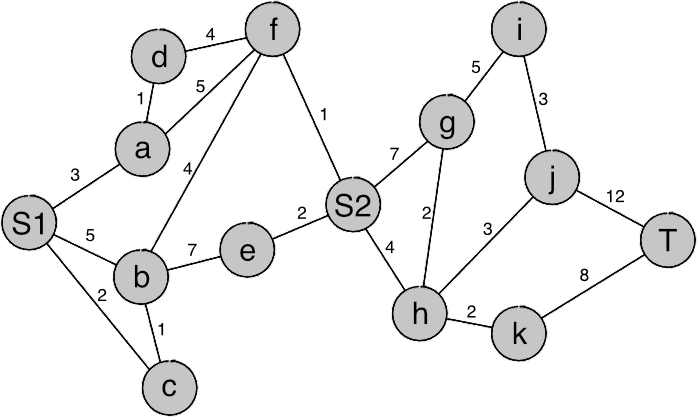
\includegraphics[scale=0.9]{chapters/informed_search/Anfangsproblem.png}
	\caption{Beispiel Graph}
\end{figure}

Wir sehen unsere Startknoten $S1$ und $S2$, sowie den Zielknoten $T$.  Au\ss erdem sind alle Kanten zwischen den Knoten mit einer L\"ange versehen. Im folgenden werden wir mit Hilfe der Breitensuche erst den Weg von $S1$ zu $T$ und dann den Weg von $S2$ zu $T$ suchen. In der folgenden Grafik sind die Zwischenknoten mit Kleinbuchstaben beschriftet, des weiteren sind Start und Ziel in gelb eingef\"arbt. In jedem Schritt werden die aktuell zu untersuchenden Knoten gr\"un und die bereits besuchten Knoten blau markiert.

\begin{figure}[h!]
	\centering
	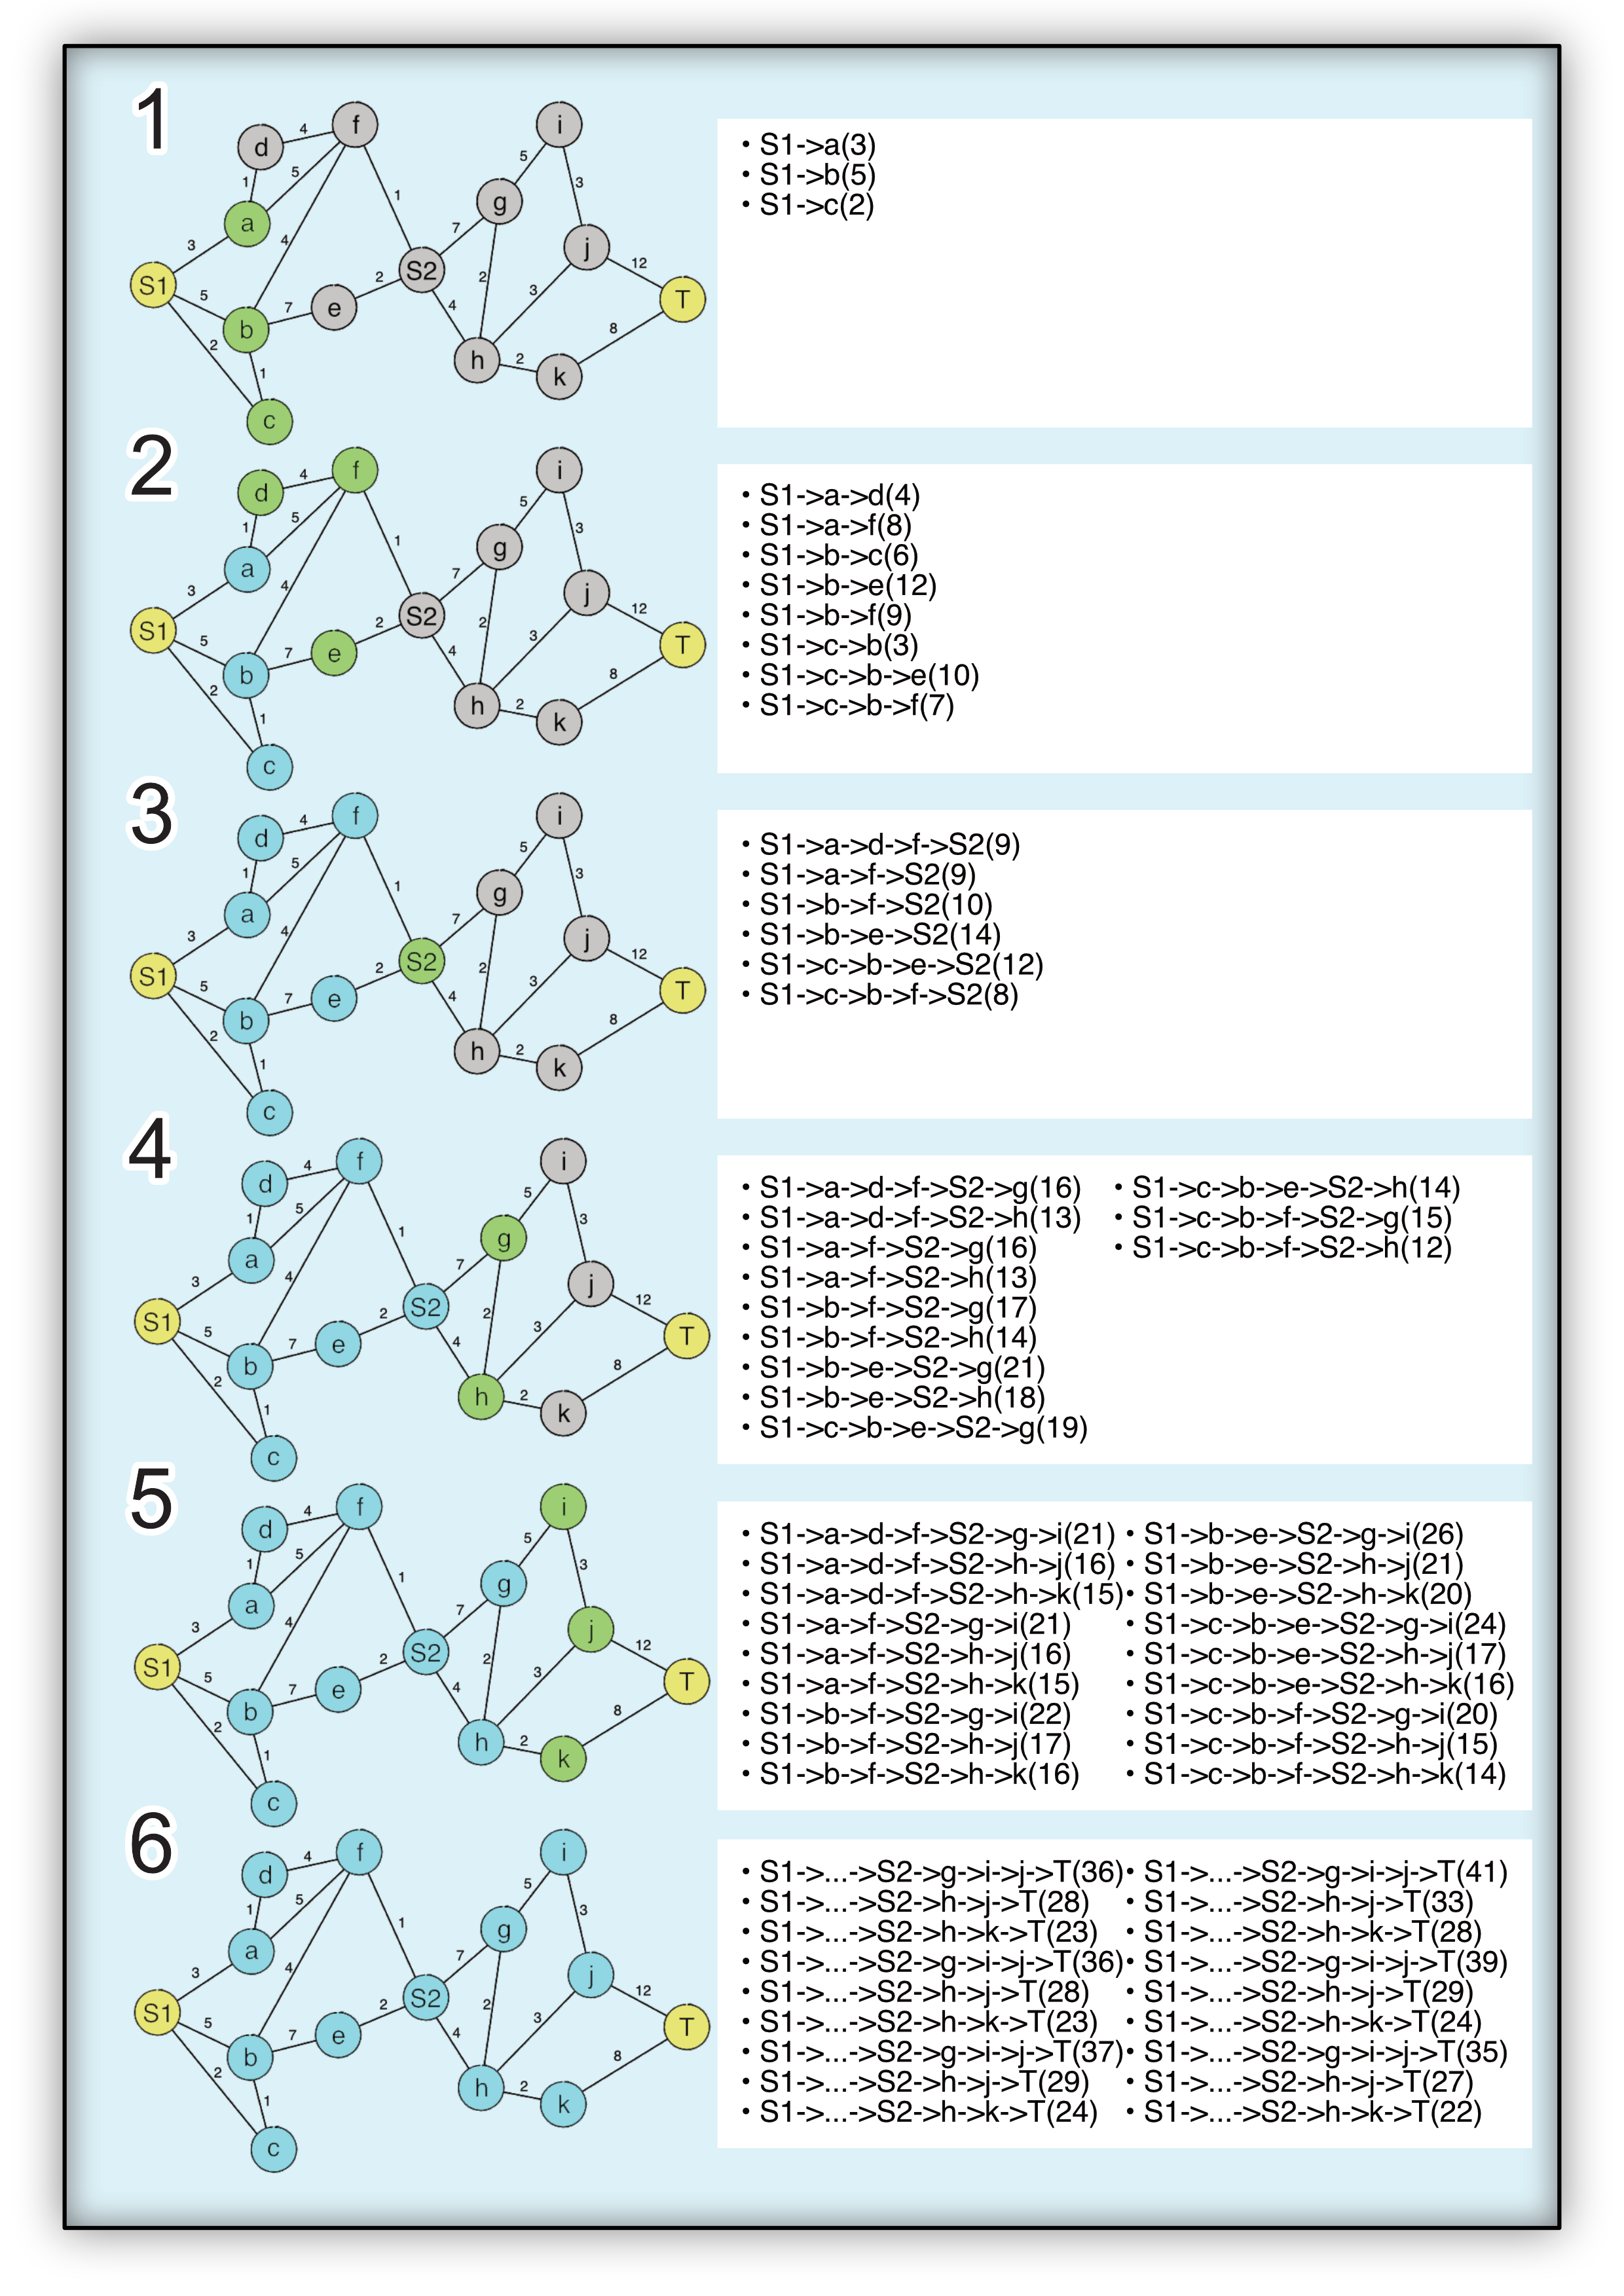
\includegraphics[scale=0.76]{chapters/informed_search/BeispielGraphen1.png}
	\caption{Beispiel Graph mit Breitensuche. Zu jedem Graphen sind die besuchten Wege angegeben. Die durch "..."\ zusammengefassten Wegst\"ucke der Wege des letzten Graphen entsprechen denen der Wegen von $S1$ nach $S2$ des vorletzten Graphens.}
\end{figure}

\begin{enumerate}
	\item Wir besuchen zuerst Knoten $a$, $b$ und $c$ und stellen offensichtlich fest, dass wir $T$ noch nicht erreicht haben. 
	\item Wir besuchen nun $d$, $e$ und $f$. Wir haben $T$ immer noch nicht erreicht.
	\item In diesem Schritt gibt es nur $S2$ zu besuchen. 
	\item Ab hier Suchen wir effektiv den k\"urzesten Weg von $S2$ zu $T$, weshalb dieses Beispiel sp\"ater nicht mehr extra erl\"autert wird. Hier besuchen wir die Knoten $g$ und $h$.
	\item Dann besuchen wir noch $i$, $j$ und $k$.
	\item Jetzt bilden wir noch die letzen Wege und diese enden beim Knoten $T$. Also sind wir fertig. 
\end{enumerate}
Der k\"urzeste Weg von $S1$ zu $T$ ist also:
\begin{itemize}
	\item  $S1\rightarrow c\rightarrow b\rightarrow f\rightarrow S2\rightarrow h\rightarrow k\rightarrow T$
\end{itemize}
Und daraus folgt der k\"urzeste Weg von S2 zu T ist: 
\begin{itemize}
	\item $S2\rightarrow h\rightarrow k\rightarrow T$
\end{itemize}
Fazit:

Wie man sieht ist das Problem gut l\"osbar mit uninformierte Suche, aber es f\"allt sofort auf das wir alle Knoten besuchen mussten und alle Wege bilden mussten.
Dies hat nicht nur hohe Speicherkosten zur Folge, sondern auch eine hohe Laufzeit. 
Bereits bei diesen simplen Beispiel sieht man die enorme Menge von Wegen die man speichern muss. 
Als Mensch w\"urde man bei dieser Suche weniger Wege betrachten:
\begin{itemize}
	\item W\"are es nicht einfacher Wege auszulassen die offensichtlich zu lang sind?
	\item Oder w\"are es nicht besser Wege wie $S1\rightarrow b$ durch den k\"urzeren $S1\rightarrow c\rightarrow b$ zu ersetzen?
\end{itemize}
Unterbewusst benutzt man eine Menge Vereinfachungen die der Computer vielleicht auch anwenden sollte. 
Im folgenden Kapitel werden wir versuchen diese Suche intuitiv zu optimieren. /newpage

\section{Verbesserungen}
\subsection{Intuitiver Algorithmus}
Statt alle Knoten zu besuchen wie bisher, werden wir im folgenden unser Wissen \"uber den Graphen nutzen um schneller zum Ergebnis zu kommen. Folgende Regeln werden angewandt:
\begin{enumerate}
	\item Wir besuchen immer den Knoten mit der niedrigsten Kantenl\"ange zuerst.
	\item Wenn wir einen neuen Weg zu einem Knoten finden und dieser k\"urzer ist als der vorherige, brauchen wir nur noch diesen neuen Weg zu betrachten. Ansonsten kann der neue Weg ignoriert werden.
	\item Wenn wir zwei Wege zur Auswahl haben, die gleichlang sind, w\"ahlen wir zuf\"allig.
	\item Wenn ein Weg keine nicht besuchten Kinder mehr hat gehen wir zur\"uck zum letzten Knoten der noch offene Kinder hatte.
	\item Aufgrund der oben genannten Regeln muss der erste Weg zum Ziel der k\"urzeste sein. (Um das Beispiel nicht unn\"otig lang zu machen, wird dies an dieser Stelle nicht bewiesen)
\end{enumerate}

\subsection{Anwendung}
Wir beginnen mit dem Graphen aus Kapitel 1. Die Knoten werden genau wie bereits bekannt eingef\"arbt werden. 

\begin{figure}[h!]
	\centering
	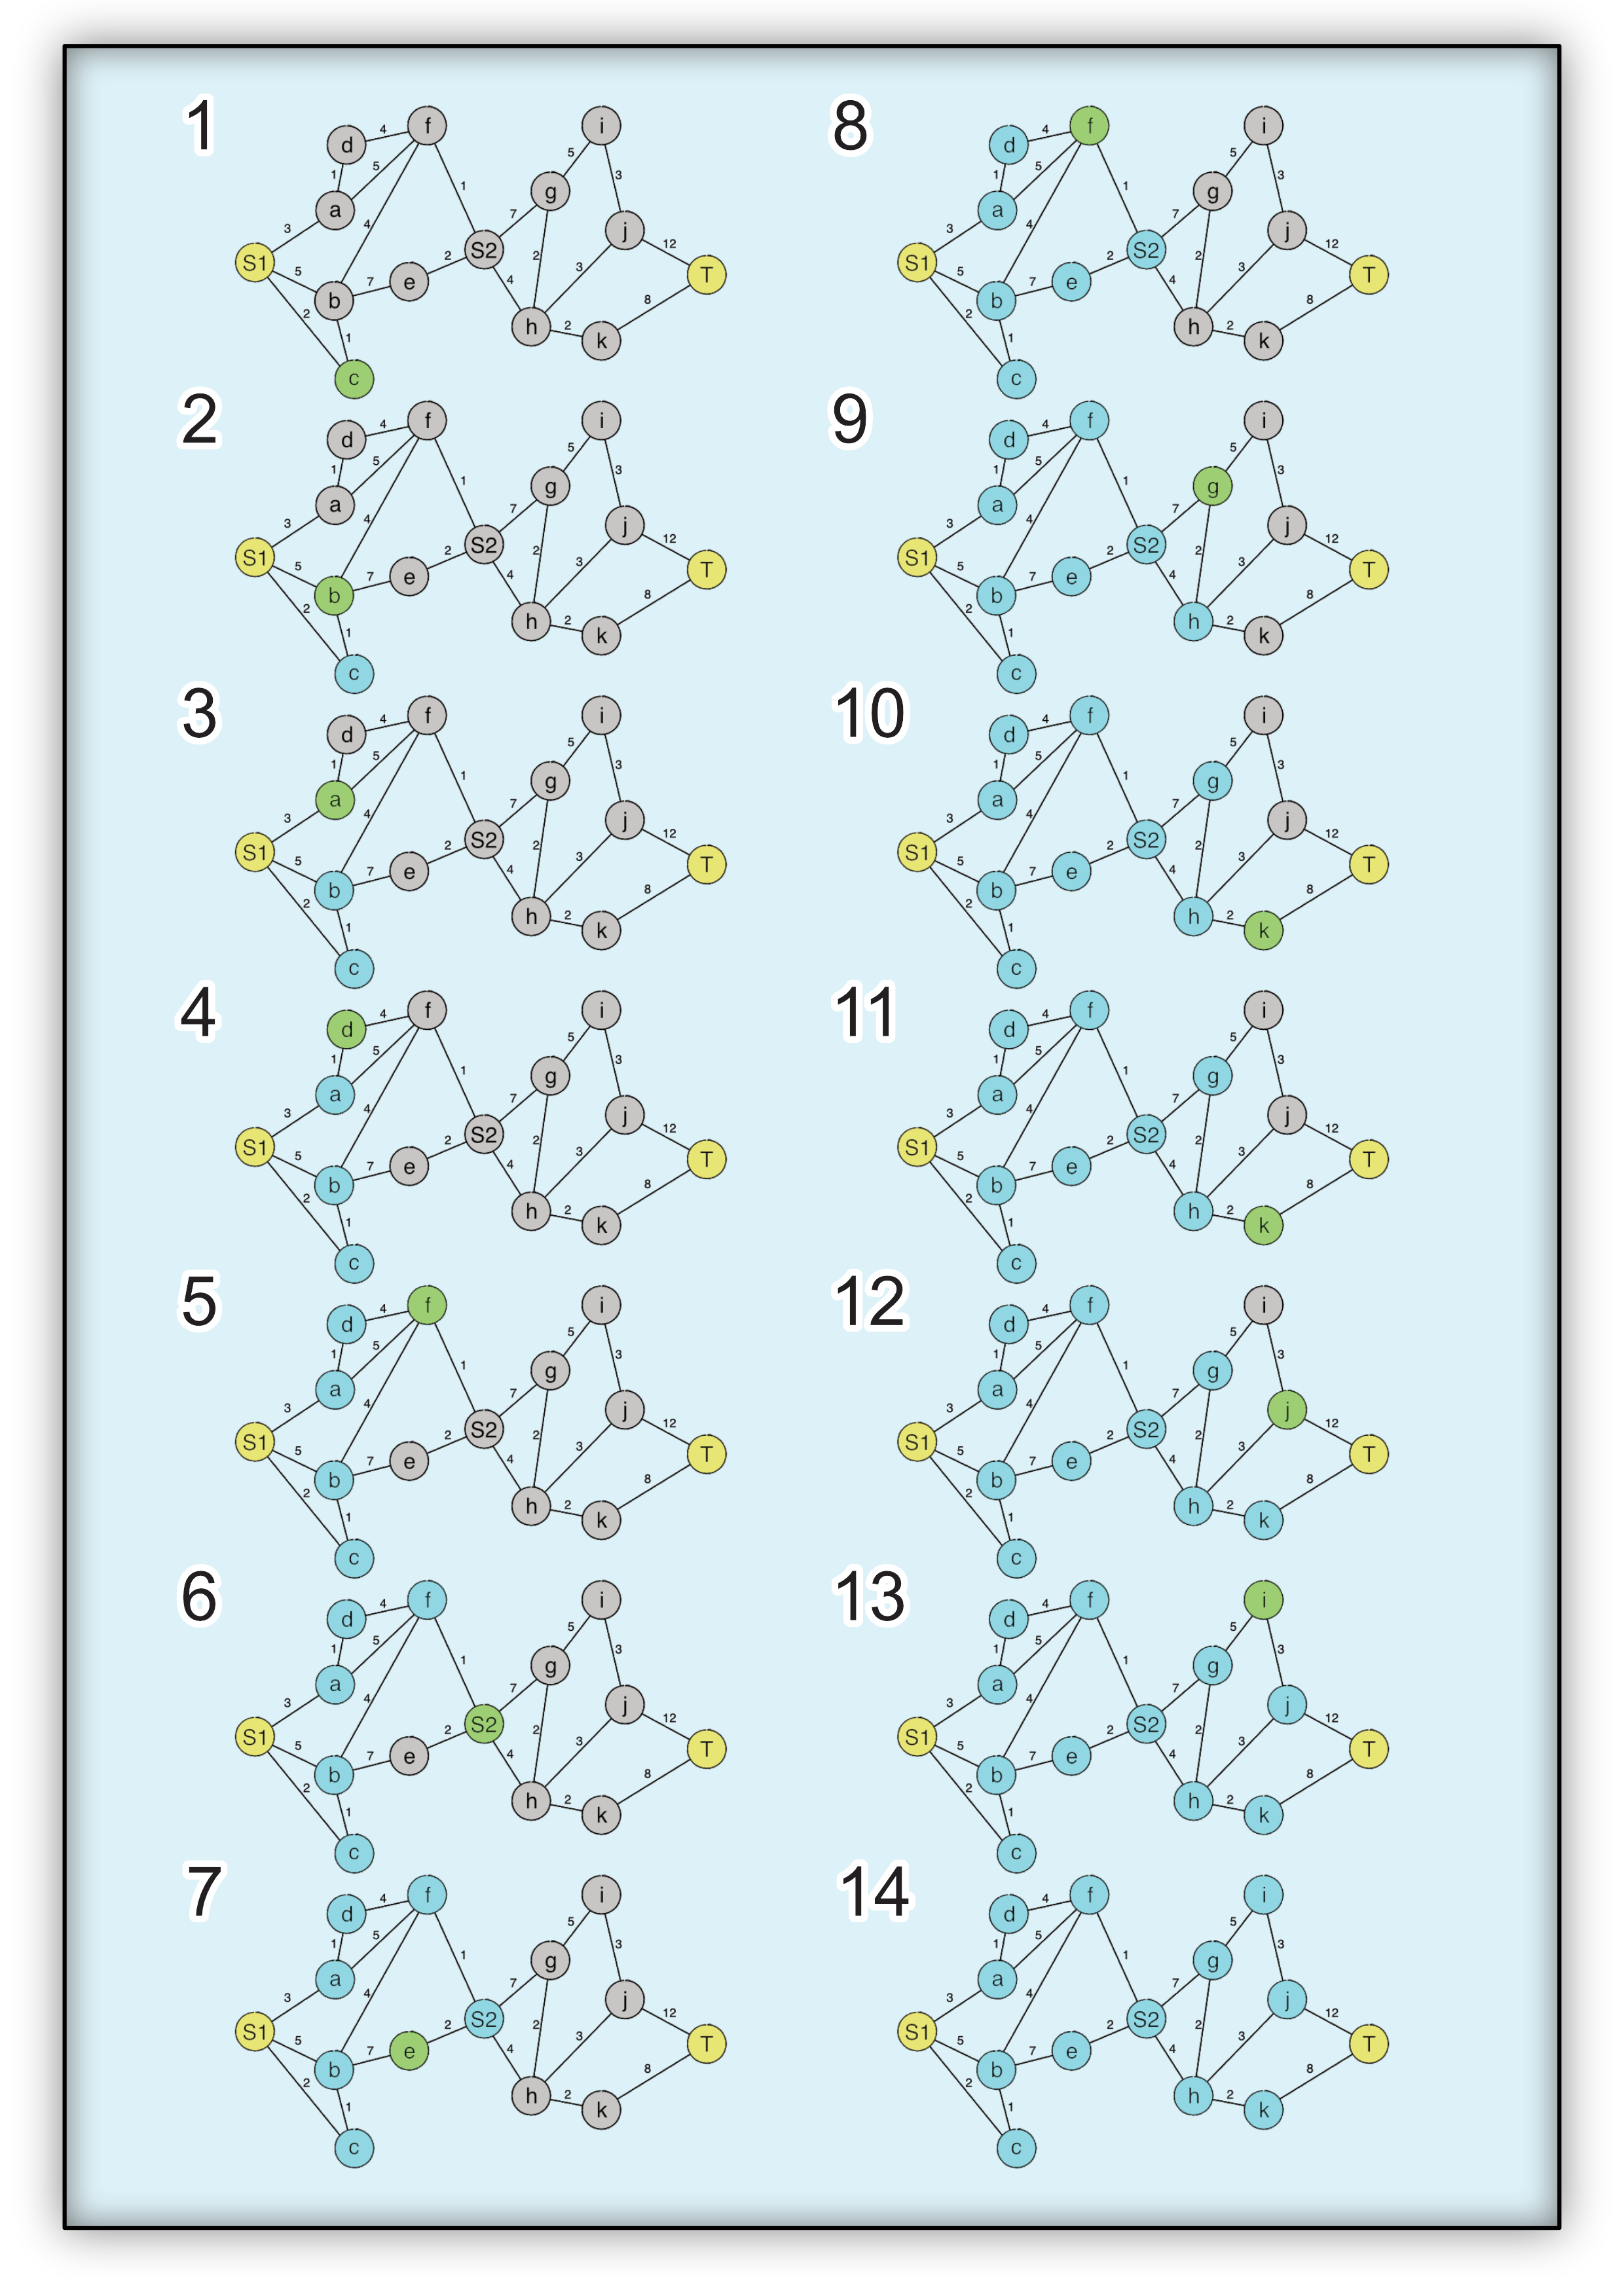
\includegraphics[scale=0.76]{chapters/informed_search/BeispielGraphen2.png}
	\caption{Beispiel Graph mit intuitiven Algorithmus.}
\end{figure}

\begin{enumerate}	\item Wir beginnen mit Knoten $c$ da mit einer L\"ange von $2$ seine Kante am k\"urzesten ist $(Regel 1)$. 
Wir haben also den Weg:
	\begin{itemize}
		\item $S1\rightarrow c(2)$
	\end {itemize}
	\item Nun besuchen wir $b$ und erhalten den Weg:
	\begin{itemize}
		\item $S1\rightarrow c\rightarrow b(3)$
	\end{itemize}
	\item Jetzt m\"ussen wir erst $a$ betrachten, da die Kante mit einer L\"ange von $3$ k\"urzer ist als $b\rightarrow f$ mit $4$. Wir haben also die Wege:
	\begin{itemize}
		\item $S1\rightarrow c\rightarrow b(3)$
		\item $S1\rightarrow a(3)$
	\end{itemize}
	\item Als n\"achstes besuchen wir $d$, da $a\rightarrow d$ am k\"urzesten ist. Es werden die Wege:
	\begin{itemize}
		\item $S1\rightarrow c\rightarrow b(3)$
		\item $S1\rightarrow a\rightarrow d(4)$
	\end{itemize}
	gespeichert.	\item Wir mussten uns zwischen $d\rightarrow f$ und $b\rightarrow f$ entscheiden und haben zuf\"allig $d\rightarrow f$ gew\"ahlt $(Regel 3)$. Damit ergeben sich die Wege:
	\begin{itemize}
		\item $S1\rightarrow c\rightarrow b(3)$
		\item $S1\rightarrow a\rightarrow d\rightarrow f(8)$
	\end{itemize}
	\item Im n\"achsten Schritt w\"ahlen wir $f\rightarrow S2$. Die Wege sind:
	\begin{itemize}
		\item $S1\rightarrow c\rightarrow b(3)$
		\item $S1\rightarrow a\rightarrow d\rightarrow f\rightarrow S2(9)$
	\end{itemize}
	\item Jetzt besuchen wir $e$. Wir haben also die Wege:
	\begin{itemize}
		\item $S1\rightarrow c\rightarrow b(3)$
		\item $S1\rightarrow a\rightarrow d\rightarrow f\rightarrow S2\rightarrow e(11)$
	\end{itemize}
	Stellen aber fest, dass $e$ f\"ur den n\"achsten Schritt keine unbesuchten Kinder hat. Also gehen wir zur\"uck zu $S2$ da dieser noch Kinder hatte $(Regel 4)$. Die Wege werden wieder zu:
	\begin{itemize}
		\item $S1\rightarrow c\rightarrow b(3)$
		\item $S1\rightarrow a\rightarrow d\rightarrow f\rightarrow S2(9)$
	\end{itemize}
	Wir besuchen noch einmal $f$, dieses Mal als $b\rightarrow f$ (zuf\"allig gew\"ahlt aus $b\rightarrow f$ und $S2\rightarrow h$). Damit haben wir einen neuen Weg zu $f$, der k\"urzer ist als $S1\rightarrow a\rightarrow d\rightarrow f$. Wir ersetzen ihn $(Regel 2)$. Damit ergibt sich der Weg:
	\begin{itemize}
		\item $S1\rightarrow c\rightarrow b\rightarrow f\rightarrow S2(8)$
	\end{itemize}	\item Wir w\"ahlen $h$ und erhalten den Weg:
	\begin{itemize}
		\item $S1\rightarrow c\rightarrow b\rightarrow f\rightarrow S2\rightarrow h(12)$
	\end{itemize}
	\item Aus $h\rightarrow g$ und $h\rightarrow k$ w\"ahlen wir $g$. Der Weg ist:
	\begin{itemize}
		\item $S1\rightarrow c\rightarrow b\rightarrow f\rightarrow S2\rightarrow h\rightarrow g(14)$
	\end{itemize}
	\item Wir besuchen $k$. Damit ergeben sich die Wege:
	\begin{itemize}
		\item $S1\rightarrow c\rightarrow b\rightarrow f\rightarrow S2\rightarrow h\rightarrow g(14)$
		\item $S1\rightarrow c\rightarrow b\rightarrow f\rightarrow S2\rightarrow h\rightarrow k(14)$
	\end{itemize}
	\item Wir w\"ahlen $j$ und erhalten die Wege: 
	\begin{itemize}
		\item $S1\rightarrow c\rightarrow b\rightarrow f\rightarrow S2\rightarrow h\rightarrow g(14)$
		\item $S1\rightarrow c\rightarrow b\rightarrow f\rightarrow S2\rightarrow h\rightarrow k(14)$
		\item $S1\rightarrow c\rightarrow b\rightarrow f\rightarrow S2\rightarrow h\rightarrow j(15)$
	\end{itemize}	\item Jetzt besuchen wir erst $j\rightarrow i$. 
	\item Dann besuchen wir sofort $g\rightarrow i$, aber wir haben \"uber $j$ bereits einen k\"urzeren Weg zu $i$ und k\"onnen den neuen ignorieren. Es folgen die Wege:
	\begin{itemize}
		\item $S1\rightarrow c\rightarrow b\rightarrow f\rightarrow S2\rightarrow h\rightarrow k(14)$
		\item $S1\rightarrow c\rightarrow b\rightarrow f\rightarrow S2\rightarrow h\rightarrow j\rightarrow i(18)$
	\end{itemize}
	Und wir sehen, dass $i$ keine Kinder mehr hat:
	\begin{itemize}
		\item $S1\rightarrow c\rightarrow b\rightarrow f\rightarrow S2\rightarrow h\rightarrow k(14)$
		\item $S1\rightarrow c\rightarrow b\rightarrow f\rightarrow S2\rightarrow h\rightarrow j(15)$
	\end{itemize}
	\item Als letztes nehmen wir noch $k \rightarrow  T$. Wir bekommen also den Weg:
	\begin{itemize}
		\item $S1 \rightarrow  c \rightarrow  b \rightarrow  f \rightarrow  S2 \rightarrow  h \rightarrow  k \rightarrow  T (22)$ 
	\end{itemize}
	und aus $Regel 5$ folgt, dass dies der k\"urzeste Weg sein muss. 
\end{enumerate}
Fazit:

Zuallererst unser Ergebnis ist identisch mit dem aus Kapitel 1, wir haben also ebenfalls den besten Weg gefunden.  Es es leicht sichtbar, dass unser intuitiver Algorithmus nicht perfekt ist. Wir mussten trotzdem alle Knoten besuchen, genau wie die Breitensuche. Aber man sieht ebenfalls sofort, dass wir deutlich weniger Wege betrachten und speichern mussten als zuvor. Und besonders hervorzuheben ist, dass wir die Suche beenden konnten als wir den ersten Weg gefunden hatten. Das wirkt sich nat\"urlich positiv auf Laufzeit und Speicherverbrauch aus. In den folgenden Kapiteln wollen wir die hier intuitiv erarbeiteten Konzepte formal definieren, die echten Algorithmen der informierten Suche vorstellen und deren Eigenschaften \"uberpr\"ufen. 
 
\section{Einleitung}
Statt blind alle M\"oglichkeiten zu probieren um die Beste zu erhalten, zieht man, wie ein Mensch es intuitiv machen w\"urde, weitere Informationen \"uber das Problem zurate (Heuristiken) und ignoriert L\"osungen die offensichtlich schlechter sind als bereits gefundene (Branch and Bound). Damit ergibt sich eine deutlich bessere Laufzeit, wie sie in Echtzeitanwendungen (z.B. in Spielen) n\"otig ist. Nat\"urlich stellt sich auch die Frage, ob diese einfacher erhaltene L\"osung immer noch die optimale L\"osung ist (Optimalit\"at). Im folgenden werden die Verschiedenen Arten (Best-First Search und A*) informierter Suche von und deren Vor- und Nachteile erkl\"art. 

\section{Definitionen}
\subsection{Branch and Bound}
Branch and Bound (h\"aufig abgek\"urzt mit B\&B\footnote{Branch and Bound Algorithms - Principles and Examples. Jens Clausen, March 12, 1999}) ist eine Optimierungsstrategie f\"ur Algorithmen, hier im speziellen Suchverfahren. Um nicht alle Knoten eines Baumes durchsuchen zu m\"ussen, kann man, wie bereits intuitiv oben gesehen, die Aufgabe in Teile aufteilen ("Branch"\ engl. "to branch" verzweigen\footnote{www.dict.cc}) und diese Teile nach Relevanz f\"ur die L\"osung einteilen ("Bound\ engl. "to bound" beschr\"anken\footnote{www.dict.cc}). 
Damit man dies bei Suchalgorithmen bewerkstelligen kann benutzt man eine Absch\"atzung, intuitiv war dies "k\"urzeste Luftlinie zum Ziel"\, auch Heuristik genannt.\footnote{Anwendungen von Branch and Bound, Frederik Wollny und Philipp Schmid, Hochschule Aalen, 2016}

\subsection{Extended List}
Bei der Anwendung von Branch and Bound kann es dazu kommen, dass Wege p'=(\dots, A) zu einen Knoten A weiter verfolgt werden, f\"ur die es einen Weg p=(\dots, A) gibt, so dass gilt:
\begin{center} 
$Wf(p) < Wf(p')$
\end{center}
Dies f\"uhrt dazu, dass der Suchbaum unn\"otig gro\ss wird. Um zu erreichen, dass nicht die l\"angeren Wege weiter verfolgt werden, wird die Extended List eingef\"uhrt. In der Extended List wird f\"ur jeden Knoten zum Zeitpunkt an dem dieser besucht wird, die Knoten Identifikation und die Wegl\"ange zu diesem gespeichert. F\"uhrt nun im Verlauf der Suche ein Weg zu einem Knoten, der bereits in der Extended List gespeichert ist, so wird die gespeicherte mit der Aktuellen Wegl\"ange zum Knoten verglichen. Ist die Aktuelle Wegl\"ange gr\"o\ss er, muss der Weg nicht weiter verfolgt werden, es gibt bereits einen k\"urzeren Weg zu dem Knoten. Ist sie geringer, wird der neue Wert eingetragen und der \"altere Weg \"uber diesen Knoten muss nicht weiter betrachtet werden.\footnote{https://ocw.mit.edu/courses/electrical-engineering-and-computer-science/6-034-artificial-intelligence-fall-2010/lecture-videos/lecture-5-search-optimal-branch-and-bound-a/} Mit Branch and Bound + Extended List ergibt sich in unserem Beispiel Graphen:

\begin{figure}[h!]
	\centering
	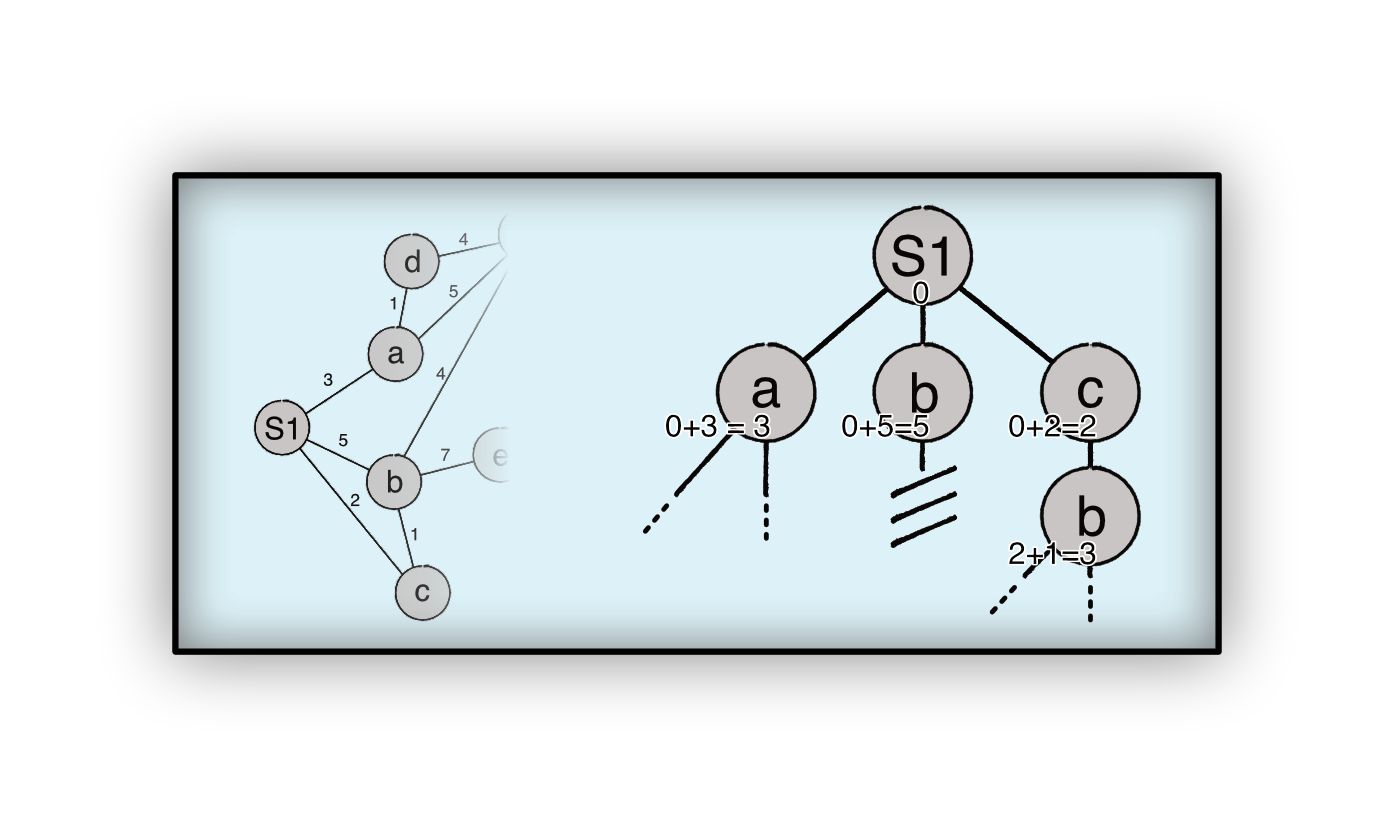
\includegraphics[scale=0.4]{chapters/informed_search/ExtendedListBeispiel.png}
	\caption{Links ist der linke Teil des Beispiel Graphen abgebildet, rechts ein Teil des Suchbaums von Branch and Bound + Extended List. Wie abgebildet wird der Weg (S1, b, \dots) nicht weiter verfolgt, da, $Wf((S1, c, b)) < Wf(S1,b)$.}
\end{figure}

\section{Best-First Search}
Best-First Search ist eine Klasse von informierten Such-Algorithmen, welche nachdem Prinzip arbeiten, dass sie stets denjenigen Knoten zuerst untersuchen, welcher f\"ur den Erfolg der Suche am "vielversprechendsten"\ erscheint. Die Wahl dieses "vielversprechenden"\ Knotens geschieht anhand einer gewissen Heuristik. Der wohl bekannteste Algorithmus aus diesem Bereich ist A*, welcher auch als eine Erweiterung von Branch and Bound gesehen werden kann. An ihm wollen wir im Folgenden das Prinzip von Best-First Search verdeutlichen. 

\section{Heuristik}
Die Heuristik ist im Falle der Informierten Suche die Representation der menschlichen L\"osungsfindung im Such-Algorithmus. Sie weist jedem Knoten einen gesch\"atzten Wert zu, der dar\"uber Auskunft gibt, ob es sich lohnen k\"onnte, einen Weg \"uber diesen Knoten einzuschlagen. Bei der Findung des k\"urzesten Weges gilt, desto h\"oher der durch die Heuristik bestimmte Wert f\"ur einen Knoten ist, desto unwahrscheinlicher ist es, dass der K\"urzeste Weg \"uber diesen Knoten verl\"auft. Aufgrund der Vielfalt von Gegebenheiten unter denen eine Suche stattfinden kann, ist es offensichtlich, dass eine Heuristik die ein Problem L\"ost nicht ohne weiteres auf andere Probleme \"ubertragen werden kann. Deswegen werden zun\"achst einige wichtige Begrifflichkeiten gekl\"art, die beim Umgang mit Heuristiken helfen k\"onnen.\footnote{http://www.duden.de/rechtschreibung/Heuristik}

\subsection{Eigenschaften von Heuristiken}
Im folgenden werden einige Eigenschaften definiert, die eine Heuristikfunktion erf\"ullen kann. Diese Eigenschaften k\"onnen dabei helfen ein Urteil, \"uber die Zul\"assigkeit einer Heuristik f\"ur eine Problemstellung, zu f\"allen.
\newtheorem*{theore}{Theorem}
\theoremstyle{definition}
\newtheorem*{defi}{Definition}

\begin{defi}
Eine heuristische Funktion $h(n)$ wird als admissible (zul\"assig) bezeichnet, wenn f\"ur alle Knoten $n$ erf\"ullt ist: 
\begin{center}
$h(m) \leq k(m, n)$
\end{center}
mit $k(m, n)$ als k\"urzeste Wegl\"ange von $m$ nach $n$ und f\"ur alle Knoten $t \in G$, die die Endbedingung erf\"ullen, gilt: 
\begin{center}
$h(t)=0.\footnote{https://ocw.mit.edu/courses/electrical-engineering-and-computer-science/6-034-artificial-intelligence-fall-2010/lecture-videos/lecture-5-search-optimal-branch-and-bound-a/}$
\end{center}
\end{defi}

Admissible Heuristiken reichen bereits aus, um auf Landkarten o.\"a. nach der k\"urzesten Route zu suchen. Damit eine Heuristik auch f\"ur Suchen verwendet werden kann die nicht auf geografischer Ebene stattfinden, werden die Eigenschaften konsistent und monoton definiert. Die Definitionen wurden aus [Kai13] \"ubernommen. 

\begin{defi}
Eine heuristische Funktion $h(n)$ ist konsistent, wenn f\"ur alle Knotenpaare $m, n \in G$ folgendes erf\"ullt ist: 
\begin{center}
$h(m) \leq k(m, n) + h(n)$
\end{center}
mit $k(m, n)$ als k\"urzeste Wegl\"ange von $m$ nach $n$ und f\"ur alle Knoten $t \in G$, die die Endbedingung erf\"ullen, gilt: 
\begin{center}
$h(t)=0$.
\end{center}
\end{defi}

\begin{defi}
Eine heuristische Funktion $h(n)$ ist monoton, wenn f\"ur alle Knotenpaare $m, n \in G$ mit $n$ als unmittelbarem Nachbar von $m$ folgendes erf\"ullt ist: 
\begin{center}
$h(m) \leq c(m, n) + h(n)$
\end{center}
mit $c(m, n)$ als Kosten der Kante von $m$ nach $n$; und f\"ur alle Knoten $t \in G$, die die Endbedingung erf\"ullen, gilt: 
\begin{center}
$h(t)=0$.
\end{center}
\end{defi}

\begin{theore}
Die Eigenschaften konsistent und monoton sind \"aquivalent.
\end{theore}

\begin{theore}
F\"ur jede konsistente Funktion $h$ gilt:
$h(n) \leq h*(n)$ f\"ur alle Knoten $n \in G$.
\end{theore}

Um den unterschied zwischen einer Heuristik die admissible ist und einer die konsistent ist zu verdeutlichen, sei ein Beispiel angef\"uhrt: 

\begin{figure}[h!]
	\centering
	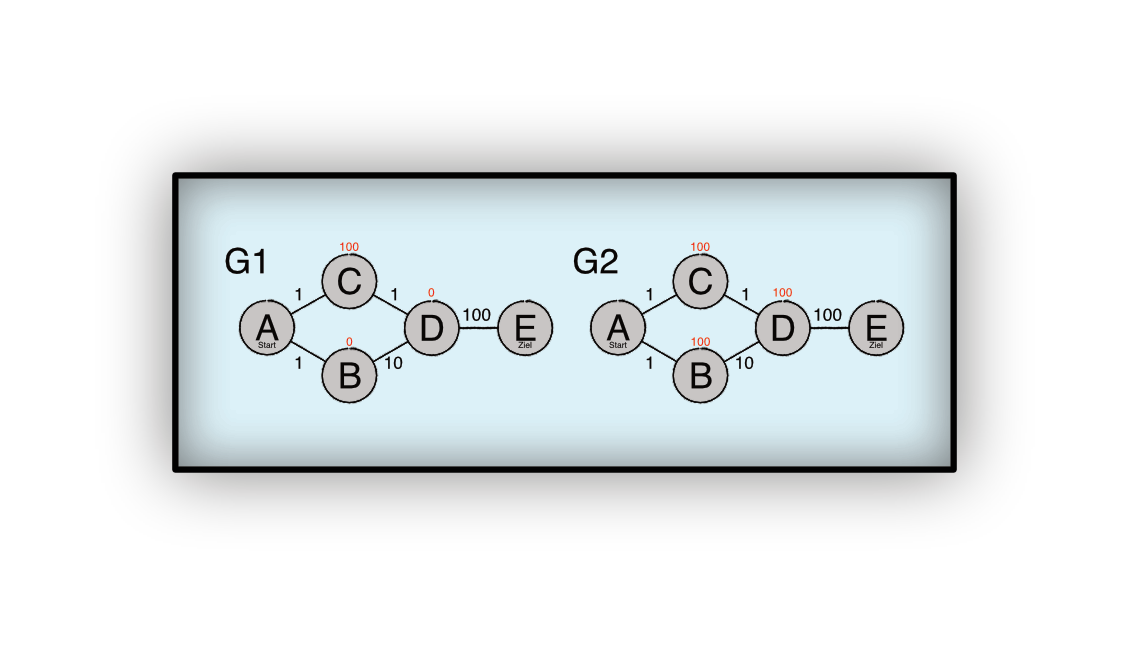
\includegraphics[scale=0.5]{chapters/informed_search/BeispielHeuristik.png}
	\caption{Die Abbildungen G1 und G2 beschreiben das selbe Problem mit zwei verschiedenen Heuristiken. Ziel ist es den k\"urzesten Weg von Knoten A nach Knoten E zu finden. G1 stellt die Verwendung einer admissible Heuristik und G2 die einer konsistenten Heuristik dar. Die roten Zahlen geben die Werte der Heuristikfunktionen an den relevanten Knoten an. Wird nun eine Suche, mit Branch and Bound + Extended List + Heuristik durchgef\"uhrt, liefert die Suche f\"ur G1 den Weg(A,B,D,E) und f\"ur G2 den Weg(A,C,D,E). Entscheidend f\"ur diese L\"osung ist, dass bei G1 zun\"achst A,B, und D betrachtet werden und somit aufgrund der Extended List der Weg (A,C,D,E) wegf\"allt. Im Gegensatz dazu beginnt die Suche bei G2 mit einem Weg \"uber C, da die gesch\"atzten Kosten von C mit 101 kleiner als die von B sind.}
\end{figure}

\subsection{Verschiedene Heuristiken}
In diesem Abschnitt werden drei Heuristiken vorgestellt, angefangen mit der Hamming-Distanz. Aufgrund dessen, dass in einigen Kapiteln Bezug auf die folgenden Heuristiken genommen wird, wurden einige Bezeichnungen in den Definitionen entsprechend angepasst.\\
Die Hamming-Distanz hh(m,n) beschreibt wie gro\ss der Unterschied zwischen den Zeichenketten m und n ist und ist wie folgt definiert: 
\begin{defi}
$\sum$ sei ein endliches Alphabet sowie $m = (m_{1}, \dots, m_{k})$ und $y = (n_{1}, \dots, n_{k})$ zwei $k$ Zeichen lange Worte aus $\sum^{k}$. Die Hamming-Distanz zwischen $m$ und $n$ ist definiert als:
\begin{center}
$h_{h}(m,n) := |{j \in \{1 , \dots , k\} | m_{j} \neq n_{j}}|$.
\end{center}
\end{defi}
Eine Heuristik w\"are z.B. $h(n)=h_{h}(n,x)$, mit $x$ als Ziel-Konstellation der Suche.\footnote{http://sb.fluomedia.org/hamming/, https://de.wikipedia.org/wiki/Hamming-Abstand}
\begin{defi}
Die Manhattan Distanz $h_{m}(m,n)$ f\"ur die Punkte $n$ und $m$ beschreibt die Distanz, die zustande kommt, wenn nur horizontale und vertikale Wege genommen werden, um $n$ von $m$ aus zu erreichen. Die Manhattan-Distanz ist wie folgt definiert:
\begin{center}
$h_{m}(m,n) = \sum_{i} |m_{i} - n_{i}|.$
\end{center}
\end{defi}
Eine Heuristik w\"are z.B $h(n)=h_{m}(n,x)$, mit $x$ als Ziel-Knoten der Suche.\footnote{http://mathworld.wolfram.com/TaxicabMetric.html}
\begin{defi}
Der Euklidischer Abstand $h_{e}(m,n)$ von $m$ und $n$ entspricht der "Luftlinie" zwischen diesen. Der Euklidische Abstand f\"ur zwei Vektoren im $k$-Dimensionalen Raum ist wie folgt definiert:
\begin{center}
$h_{e}(m,n) =\sqrt{((m_{1} - n_{1})^{2}+\dots+(m_{k} - n_{k})^{2})}.$
\end{center}
\end{defi}
Eine Heuristik w\"are z.B $h(n)= h_{e}(n,x)$, mit $x$ als Ziel-Knoten der Suche.\footnote{http://mathworld.wolfram.com/EuclideanMetric.html}

\subsection{Findung von Bewertungsfunktionen}
Die Frage Lautet:"Wie findet sich die richtige Heuristikfunktion f\"ur die gegebene Problemstellung". Um einen L\"osungsansatz f\"ur eine allgemeine Vorgehensweise zu finden, wird zun\"achst das Beispiel aus 5.1 betrachtet. Die Aufgabe im Beispiel ist es, den k\"urzesten Weg von dem Knoten S1 bzw. S2 zum Zielknoten T im Graphen zu finden. Die Problemstellung l\"asst sich in eine Konjunktion von zwei Bedingungen aufteilen:
\begin{enumerate}
	\item Die zur\"uckgelegte Strecke von S1 bzw. S2 nach T soll minimal sein.
	\item Die Strecke entspricht einem Weg (Graphentheorie).
\end{enumerate}
W\"urde die zweite Bedingung weggelassen, w\"urde immer eine Strecke entsprechend der Luftlinie von $S1$ bzw. $S2$ nach $T$ gew\"ahlt werden. Es liegt also nahe $h(n)=h_{e}(n,x)$ zu w\"ahlen, um einem Knoten nach seiner Distanz zu $T$ zu bewerten. Wird Bedingung zwei nun hinzugezogen, werden mit der gew\"ahlten Heuristik immer die erreichbaren Knoten bevorzugt, die am n\"achsten zum Ziel liegen. So ist eine Akzeptable Heuristik f\"ur die Problemstellung gefunden. Dieses Prinzip des Konstruieren von vereinfachten Modellen durch systematisches Weglassen von Bedingungen der Konjunktion der Problemstellung scheint auch allgemein eine gute Herangehensweise zu sein, um leicht heuristische Sch\"atzungen zu ermitteln.

\section{A* Algorithmus}
A* beschreibt eine Gruppe von Algorithmen, die auf alle Kniffe der Informierten Suche, die bis jetzt vorgestellt wurden, zur\"uckgreifen:\footnote{https://ocw.mit.edu/courses/electrical-engineering-and-computer-science/6-034-artificial-intelligence-fall-2010/lecture-videos/lecture-5-search-optimal-branch-and-bound-a/}
\begin{itemize}
	\item Branch and Bound
	\item Extended List
	\item Heuristik
\end{itemize}
F\"ur ein gegebenes Problem gibt es innerhalb dieser Gruppe bessere und schlechtere Algorithmen. Um zwei A* Algorithmen zu vergleichen hilft das folgende Theorem: 

\begin{theore}
A*1 und A*2 seien zwei Versionen von A* mit $h1(n) ? h*(n)$ und $h2(n) ? h*(n)$ f\"ur alle Knoten $n \in G$ und mit $h1(n) ? h2(n)$ f\"ur alle Knoten $n \in G \ {t | t erf\"ullt die Endbedingung }$. (A*2 sei "besser informiert" als A*1.) Falls es eine L\"osung gibt, so wird bis zur Terminierung jeder von A*2 expandierte Knoten auch von A*1 expandiert, (A*2 "dominiert" A*1.)\footnote{[Kai13]} 
\end{theore}

In den folgenden Abschnitten wird auf weitere Eigenschaften des A* eingegangen und anschlie\ss end wird der A* durch Beispiele veranschaulicht. 

\subsection{Zul\"assigkeit}
Welche Bedingungen muss eine Heuristik erf\"ullen, damit unser Such-Verfahren ordnungsgem\"a\ss funktioniert? Dazu sollten wir zuerst definieren, wie wir uns ein korrekte Funktionsweise vorstellen.
\begin{itemize}
	\item Zul\"assigkeit Ein Such-Verfahren hei\ss t zul\"assig, falls es stets mit einer optimalen L\"osung terminiert, falls diese existiert.
\end{itemize}
Da bei unserem heuristischen Such-Verfahren A* die Wahl der Heuristik bisher nicht klar eingeschr\"ankt ist, liegt es nahe, dass in dieser Wahl ein entscheidender Punkt f\"ur die Zul\"assigkeit unseres Algorithmus liegt. Man kann sich leicht Heuristiken \"uberlegen, welche die Funktionsweise von A* st\"oren und daf\"ur sorgen, dass der Algorithmus keine optimale L\"osung findet oder wom\"oglich gar nicht erst terminiert. Wir sollten uns also genauer mit der Beschaffenheit von Heuristikfunktionen auseinandersetzen. Eine erste wichtige Eigenschaft einer Heuristik h zur Sch\"atzung von h* ist, ob diese optimistisch sch\"atzt.
\begin{itemize}
	\item optimistische Sch\"atzung Eine Sch\"atzung h von h* ist genau dann eine optimistische Sch\"atzung, falls sie die Kosten eines optimalen Pfades nie \"ubersch\"atzt.
\end{itemize}
Das heisst:
\begin{itemize}
	\item $h(n) \leq h*(n)$ f\"ur alle Knoten $n \in GP$
\end{itemize}

Diese Eigenschaft liefert uns nun die ausschlaggebende Bedingung f\"ur die Zul\"assigkeit von A*. Zul\"assigkeit von A*. Falls die verwendete Heuristik h eine optimistische Sch\"atzung von h* ist, dann ist A* zul\"assig. 
Der Beweis dieses Satzes und einige genauere Er\"orterungen k\"onnen in [Kai13] nachgelesen werden. 

\subsection{Komplexit\"at}
Es l\"asst sich leicht erkennen, dass A* in der Regel eine weit bessere Komplexit\"at hat, als blinde Such-Verfahren. Die Anzahl der expandierten Knoten ist bei A* oft sogar um ein Vielfaches geringer. Sei nun die L\"ange einer optimalen L\"osung mit d bezeichnet. Des Weiteren kann man von Einheitskosten ausgehen und die Existenz genau einer optimalen L\"osung voraussetzen. Je nachdem wie optimistisch nun der Fehler von h bez\"uglich h* angenommen wird, kommt man auf eine quadratische oder sogar lineare Komplexit\"at bez\"uglich d. Im eher realistischen Fall l\"asst sich jedoch nur auf eine exponentielle Komplexit\"at schliessen. 

\subsection{Optimalit\"at}
Nun interessieren wir uns f\"ur die Optimalit\"at von A* im Hinblick auf die Anzahl der expandierten Knoten. Der Begriff Optimalit\"at beruht hier auf dem der Dominanz. Das bedeutet, ein Verfahren ist optimal gegen\"uber einer Klasse von Verfahren, wenn es alle Elemente aus dieser Klasse dominiert. F\"ur den ganz allgemeinen Fall l\"asst sich leicht erkennen, dass A* nicht das optimale Verfahren \"uberhaupt ist. Es gibt in bestimmten F\"allen offensichtlich Verfahren, welche nicht alle von A* untersuchten Knoten ebenfalls untersuchen. Gerade bei speziell auf eine Klasse von Graphen abgestimmten Verfahren ist dies der Fall. Jedoch ist unter bestimmten Einschr\"ankungen eine konkretere Aussage bez\"uglich der Optimalit\"at von A* m\"oglich. Daf\"ur schr\"ankt man die Bedingungen auf eine Dom\"ane ein, welche eine konsistente Heuristik h besitzt, und setzt voraus, dass es mindestens einen optimalen L\"osungspfad gibt, bei welchem h < h* f\"ur alle Knoten au\ss er dem Zielknoten gilt. Dann gilt, dass A* dominant f\"ur alle Problem-Instanzen ist, und zwar f\"ur alle m\"oglichen Entscheidungsregeln bei Nicht-Eindeutigkeit des Knotens mit minimalem f-Wert. Da dem Algorithmus A* bei konsistentem h zus\"atzlich eine sehr gute Verwaltung des Suchbaumes m\"oglich ist, l\"asst sich sagen, dass A* unter diesen Voraussetzungen sehr effektiv ist. 

\subsection{Beispiel des 8-Puzzles}
Beim 8-Puzzle handelt es sich um ein Spiel, bestehend aus einem Spielbrett der Gr\"o\ss e 3-mal-3 und acht Kacheln, nummeriert von 1 bis 8, welche auf dem Spielbrett verteilt sind. Ein Feld des Spielbrettes bleibt also frei. Grenzt eine Kachel an dieses freie Feld, so kann sie an dessen Stelle verschoben werden. Das Ziel des Spieles ist, von einer ungeordneten Stellung der Kacheln durch eine Folge von Verschiebungen zu einer Zielstellung zu gelangen. Die folgende Abbildung zeigt ein konkretes Problem mittels Start- und Zielkonfiguration.
\begin{center}\includegraphics[scale=0.7]{chapters/informed_search/startziel.png}\end{center}
Die Problemstellung ist, zu einer gegebenen Kachelkonstellation die k\"urzeste Abfolge von Verschiebungen zu finden, die n\"otig ist, um zur Zielkonfiguration zu gelangen.

Wird das Problem abstrakt betrachtet, ist es m\"oglich einen Graphen zu konstruieren, auf den eine informierte Suche angewendet werden kann. Die Knoten des Graphen repr\"asentieren die Konstellationen die das Kachelfelde annehmen kann und zwei Knoten sind genau dann \"uber eine Kante miteinander verbunden, wenn sich die Kachelkonstellationen der Knoten um genau 1 Verschiebung unterscheidet. Als Kantenbewertung $f:E \rightarrow \Re$ wird die Anzahl der Verschiebungen gew\"ahlt die n\"otig ist, um die Kachelkonstellation des Zielknotens zu erhalten. In dem konstruierten Graphen ist die l\"ange jeder Kante 1.

Auf den so erhaltenen Graphen l\"asst sich nun eine informierte Suche mit einem A* Algorithmus durchf\"uhren. Um die Heuristik des A* leichter zu bestimmen, wird die Problemstellung in eine
Konjunktion aus den folgenden Bedingungen zerlegt:
\begin{enumerate}
	\item Die Anzahl der Verschiebungen soll minimal sein.
	\item Es d\"urfen nur Kacheln auf benachbarte Felder verschoben werden.
	\item Das benachbarte Feld muss leer sein.
\end{enumerate}
F\"ur Bedingung 1 bietet sich die Hamming-Distanz an. Diese gibt f\"ur jede Kachelkonstellation die Anzahl der falsch positionierten Felder an. Wird nun die 2 Bedingung hinzugezogen, muss ber\"ucksichtigt werden, dass keine diagonalen Z\"uge m\"oglich sind. Durch diese Versch\"arfung ist die Manhattan-Distanz eine passendere Heuristik. Die Manhattan-Distanz berechnet f\"ur eine gegebene Kachelkonstellation die Anzahl der horizontalen und vertikalen Verschiebungen, die n\"otig sind, um die Zielkonstellation zu erhalten. Wird zuletzt noch die 3 Bedingung hinzugezogen kann bei der Manhattan Distanz verblieben werden. Nichts desto trotz k\"onnen beide Heuristiken f\"ur das Problem verwendet werden und dies wird auch getan. Im folgenden bezeichnet die Heuristikfunktion\dots 
\begin{itemize}
	\item $h_{1}(n)$, die Anzahl falsch positionierter Kacheln in der durch Knoten n dargestellten Konfiguration (Hamming-Distanz)
	\item $h_{2}(n)$, die Summe der Distanzen der falsch positionierten Kacheln zu ihrer Zielposition (Manhattan-Distanz)
\end{itemize}
Der Ablauf des Algorithmus unter Verwendung von $h_{1}(n)$ bzw. $h_{2}(n)$ wird durch die Suchb\"aume $G_{S1}$ bzw. $G_{S2}$ dargestellt. $g$ bezeichnet die zur\"uckgelegte Wegstrecke, $h$ den Wert von $h_{1}(n)$ bzw. $h_{2}(n)$ f\"ur die gegebene Kachelkonstellation und $f$ die Summe von $h$ und $g$.

Wie an den folgenden beiden Suchb\"aumen zu sehen, ben\"otigt der A* Algorithmus unter Verwendung von $h_{2}(n)$ eine geringere Anzahl von Expansionen als bei der Verwendung von $h_{1}(n)$ ). Der Aufwand ist also geringer. Die Wahl des zu expandierenden Knotens ist stets eindeutig. Heuristik $h_{2}(n)$ scheint also ein besserer Sch\"atzer zu sein als $h_{1}(n)$. 
\begin{figure}[h!]
	\centering
	\includegraphics[scale=0.45]{chapters/informed_search/tree1.png}
	\caption{Suchbaum $G_{S1}$ zu $h_{1}$}
\end{figure}
\begin{figure}[h!]
	\centering
	\includegraphics[scale=0.65]{chapters/informed_search/tree2.png}
	\caption{Suchbaum $G_{S2}$ zu $h_{2}$}
\end{figure} 
\subsection{A* am Beispiel Graphen}
Abschlie\ss end soll ein A* Algorithmus f\"ur das in Abschnitt 6.1 pr\"asentierte Problem entworfen werden. Branch and Bound + Extended List wird wie beschrieben verwendet, die Heuristikfunktion 
\begin{center}
$h(n) = h_{e}(n,x) =sqrt((n^{1} - x^{1})^{2}+\dots+(n^{k} - x^{k})^{2})$, mit $x$ als Ziel-Knoten der Suche, 
\end{center}
wird f\"ur die Problemstellung \"ubernommen. Da es sich um die vereinfachte representation einer Karte handelt, wird $k=2$ gew\"ahlt. Der resultierende Graph mit den in rot durch die Heuristik bestimmten Werten: 

\begin{figure}[h!]
	\centering
	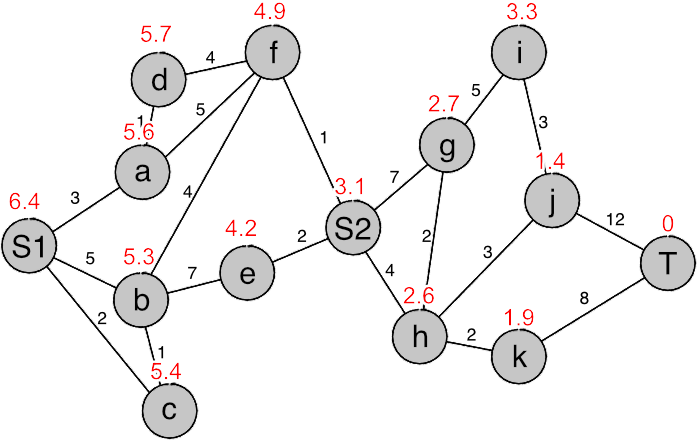
\includegraphics[scale=0.9]{chapters/informed_search/AnfangsproblemHeuristik.png}
	\caption{Beispiel Graph mit Heuristik}
\end{figure}

F\"ur die Suche des k\"urzesten Weges von S1 bzw. S2 nach T ergeben sich die beiden Suchb\"aume B1 (Abbildung6.9) und B2 (Abbildung6.10). Die in blau gekennzeichneten Zahlen geben die Reihenfolge an in der die Pfade begangen werden. Rote Zahlen geben den von der Heuristik gesch\"atzten Wert f\"ur den entsprechenden Knoten an. Die Schwarzen Zahlen geben die tats\"achliche Wegl\"ange vom Startknoten zum betrachteten Knoten an. In lila werden die gesch\"atzten Gesamtkosten eines Knotens angegeben. Als Grau markierte Pfade wurden aufgrund der Extended List ausgeschlossen.

An beiden Suchb\"aumen ist gut zu erkennen, dass viele Abzweigungen aufgrund der Extended List nahezu sofort abgeschnitten werden (gekennzeichnet durch graue Pfade). Am Baum mit Wurzel S2 l\"asst sich der nutzen einer Heuristik nachvollziehen. Die Kosten der Abzweigungen e, f in den linken Teil des Graphen nehmen durch die Heuristik schneller zu und dies sorgt daf\"ur, dass eine Suche dort obsolet (auch durch graue Pfade gekennzeichnet) wird, sobald die gesch\"atzten Kosten gr\"o\ss er als 14 sind (Der k\"urzeste Weg von S2 nach T hat die l\"ange 14). 
Die unterschiedliche Struktur der B\"aume l\"asst sich durch den Startpunkt der Suche erkl\"aren. Aufgrund dessen, dass die Knoten S1 und T auf entgegengesetzten Seiten des Graphen liegen, ergibt sich ein tiefer Baum und da der Knoten S2 den Graphen in zwei Partitionen auftrennt, bildet sich bei der Suche des k\"urzesten Weges von S2 nach T ein breiter Suchbaum. 
\begin{figure}[h!]
	\centering
	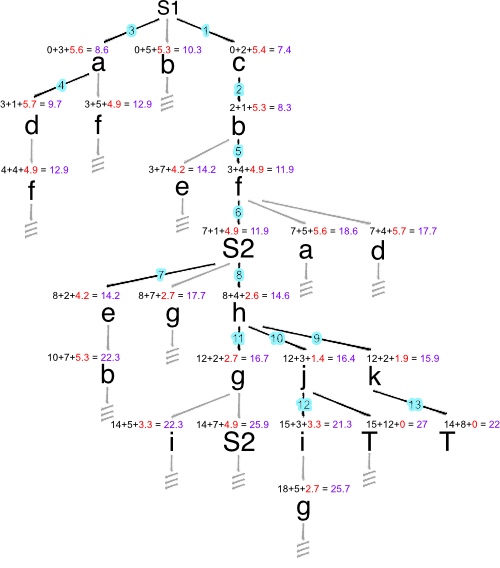
\includegraphics[scale=0.9]{chapters/informed_search/AStarBaum1.png}
	\caption{Such Baum B1 von T nach S1}
	\label{fig:searchtrees1}
\end{figure}

\begin{figure}[h!]
	\centering
	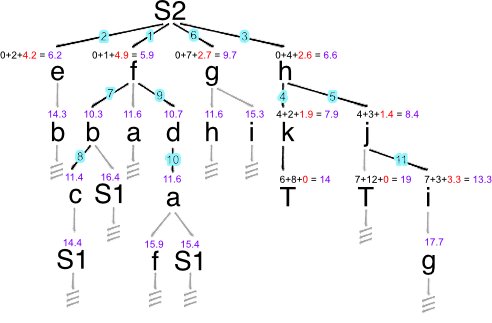
\includegraphics[scale=0.9]{chapters/informed_search/AStarBaum2.png}
	\caption{Such Baum B2 von T nach S2}
	\label{fig:searchtrees2}
\end{figure}
\newpage 
\chapterimage{chapter_head_1.png}

\chapter{Suchalgorithmen für Spiele}

\usetikzlibrary{arrows}
\usetikzlibrary{calc}
\usetikzlibrary{positioning}
\usetikzlibrary{matrix}

\pgfdeclarelayer{background}
\pgfsetlayers{background,main}

\tikzset{
    treenode/.style = {align=center, inner sep=0pt, text centered,
        font=\sffamily},
    arn_n/.style = {treenode, circle, white, font=\sffamily\bfseries, draw=blue, fill=blue,
        text width=1.5em, minimum width=1.5em, minimum height=1.5em},% arbre rouge noir, noeud noir
    arn_r/.style = {treenode, circle, white, draw=red, fill=red,
        text width=1.5em, very thick, minimum width=1.5em, minimum height=1.5em},% arbre rouge noir, noeud rouge
    arn_x/.style = {treenode, rectangle, draw=black,
        minimum width=1.5em, minimum height=1.5em},% arbre rouge noir, nil
}


\section{Intro \& Motivation}

In den vorangegangenen Kapiteln haben wir schon einige Suchverfahren kennengelernt, welche uns nun helfen werden Algorithmen zu verstehen, die verwendet werden um Computergegner für Nullsummenspiele zu entwickeln. Hierbei werden wir uns den Minimax-Algorithmus, sowie den Alpha-Beta-Algorithmus genauer anschauen, welche beide versuchen sich in die Lage des Gegners zu versetzen, um so  herauszufinden, welche Reaktion dieser auf einen Zug von uns wählen würde. Ziel der Algorithmen ist es, ein für uns bestmögliches Ergebnis und somit, wenn möglich, einen Sieg zu erlangen. Dieses Vorgehen kann eine Betrachtung von sehr vielen möglichen Zügen zur Folge haben, was sehr viel Rechenaufwand bedeutet. Im Folgenden werden wir jedoch  mit Hilfe des Alpha-Beta-Algorithmus eine Methode kennenlernen, die es uns ermöglicht die Anzahl der zu betrachtenden Züge zu reduzieren.



\section{Inhaltliche Ausarbeitung des Themas}

Wir betrachten ein Nullsummenspiel, was bedeutet, dass der Gewinn des einen Spielers (Nutzwert positiv) mit dem Verlust des Gegners (Nutzwert negativ) äquivalent ist und ein Unentschieden keine Auswirkungen auf die Nullsummeneigenschaft hat (Nutzwert 0).
Gegeben sei für dieses Spiel ein Spielbaum $T = (V;E)$. Bei einem gleichförmigen Spielbaum besitzt jeder innere Knoten den gleichen Verzweigungsgrad b und alle Blätter befinden sich in der gleichen Tiefe d, sodass die Zahl der Knoten in einem gleichförmigen Baum exponentiell mit der Tiefe des Baumes wächst ($b^d$). Jedoch gibt es auch Spielbäume bei denen der Verzweigungsgrad der Ebenen variiert.
Der Spielbaum beinhaltet alle möglichen Züge und Spielausgänge. Die Tiefe und der Verzweigungsgrad hängt von dem Spiel ab, welches wir betrachten. Beispielsweise hat der Spielbaum zu einem Tic-Tac-Toe Spiel eine Tiefe von 9 (da es 9 Felder zu besetzen gibt) und zu Beginn des Spiels einen Verzweigungsgrad von 9 (weil noch alle 9 Felder zur Auswahl stehen), der mit wachsender Tiefe allerdings abnimmt, da nach jedem Zug immer ein leeres Feld weniger vorhanden ist.



\subsection{Problemstellung}
Zu dem gegebenen Nullsummenspiel wollen wir einen Computergegner programmieren, der in der Lage ist die optimale Antwort auf jede Spielposition, bei optimalem Spiel beider Spieler, zu finden.
Dafür müssen wir jedoch vorher festlegen, was für uns optimal in diesem Zusammenhang bedeutet. Wir gehen davon aus, dass der Gegner immer den für ihn optimalen Zug wählt, d.~h. den Zug, der für ihn zum besten Nutzwert und somit für uns zum schlechtesten Nutzwert führt. Analog wollen wir agieren. Wie dies genau funktioniert werden wir im folgenden Abschnitt sehen.



\subsection{Methoden}


\subsubsection*{Minimax Algorithmus}
Im folgenden bezeichnen wir unseren Spieler mit MAX und den gegnerischen Spieler mit MIN. Wie zuvor schon angedeutet ist das Ziel des Minimax-Algorithmus den Minimax-Wert für die aktuelle Stellung zu bestimmen. Der Minimax-Wert der Endstellungen (Blätter) entspricht dem Nutzwert für MAX. Die Berechnung der anderen Knoten erfolgt rekursiv mit Hilfe der folgenden Bewertungsfunktion:

\begin{center}
	$Minimax(k) = \begin{cases} Nutzwert(k) & \mathrm{falls}~k~\mathrm{Endzustand}\\
		max\{minimax(t) ~|~ t \in N(t)\} 	& \mathrm{falls}~k~\mathrm{MAX\hbox{-}Knoten}\\
		min\{minimax(t) ~|~ t \in N(t)\}	& \mathrm{falls}~k~\mathrm{MIN\hbox{-}Knoten}	\end{cases} $
\end{center}

wobei $N(t)$ die Funktion ist, die die Kinder im Baum liefert. Die Auswertung der Knoten geschieht Bottom up, das bedeutet wir beginnen bei den Blättern und bewerten von dort ausgehend die Elternknoten und anschließend deren Eltern bis wir irgendwann bei der Wurzel angelangt sind. Der Minimax Algorithmus liefert nicht unbedingt den höchsten Nutzwert der Blätter, sondern den größten Nutzwert den man erhalten kann, wenn der Gegner selbst versucht zu gewinnen und somit den Nutzwert für uns möglichst klein zu halten.\\

Anschaulicher wird das ganze, wenn man sich den Algorithmus an einem Beispiel anschaut.

\textbf{Beispiel}\\

Gegeben sei der folgende Spielbaum
\begin{center}
\includegraphics[width = 7 cm]{chapters/minimax/jpg/Graph-Minmax1.jpg}
\end{center}

Angenommen MIN wäre an der markierten Position:
\begin{center}
	\includegraphics[width = 7 cm]{chapters/minimax/jpg/Graph-Minmax2-1.jpg}
\end{center}

Dann würde MIN den Zug auswählen, der für ihn den größten Nutzwert und somit für uns den kleinsten Nutzwert hat. Das heißt in dem Fall:
\begin{center}
	 $min\{minimax(t) | t \in N(t)\} ~=~ min\{9,3\} ~=~ 3$

\includegraphics[width = 7 cm]{chapters/minimax/jpg/Graph-Minmax2-2.jpg}
\end{center}

Angenommen MIN wäre an der markierten Position:
\begin{center}
	\includegraphics[width = 7 cm]{chapters/minimax/jpg/Graph-Minmax2-3.jpg}
\end{center}

Dann würde MIN den Zug auswählen, der für ihn den größten Nutzwert und somit für uns den kleinsten Nutzwert hat. Das heißt in dem Fall:
\begin{center}
	$min\{minimax(t) | t \in N(t)\} ~=~ min\{1,5\} ~=~ 1$

	\includegraphics[width = 7 cm]{chapters/minimax/jpg/Graph-Minmax2-4.jpg}
\end{center}

Nun betrachten wir den Zug von MAX. Der Suchbaum sieht wie folgt aus

\begin{center}
	\includegraphics[width = 7 cm]{chapters/minimax/jpg/Graph-Minmax2.jpg}
\end{center}

MAX würde den Zug wählen, der für ihn den höchsten Nutzwert hat.\\

\begin{center}
	$max\{minimax(t) | t \in N(t)\} ~=~ max\{3,1\} ~=~ 3$
	\includegraphics[width = 7 cm]{chapters/minimax/jpg/Graph-Minmax3.jpg}
\end{center}

Somit sieht der Suchbaum nach Abschluss des Minimax-Algorithmus wie folgt aus, wobei der rote Pfad den optimalen Nutzwert liefert, wenn beide Spieler optimal spielen. Somit sollte MAX den linken Knoten wählen.

\begin{center}
	\includegraphics[width = 7 cm]{chapters/minimax/jpg/Graph-Minmax4.jpg}
\end{center}

\vskip 60pt



\subsubsection*{Problem:} Der Minimax-Algorithmus durchsucht den Suchbaum $T=(V, E)$ mit Tiefensuche, in der Zeit $O(max \{|V|, |E|\}) = O(|V|)$. Somit benötigt die Suche zwar lineare Zeit, jedoch wächst der Baum exponentiell mit zunehmender Tiefe ($O(|V|)=O(b^d)$). Somit ist der Algorithmus für Bäume mit großer Tiefe ineffizient.


\subsubsection*{Alpha-Beta-Algorithmus}
 Der Alpha-Beta-Algorithmus ist eine Verbesserung vom Minimax-Algorithmus, da die Zugriffsanzahl reduziert wird, indem Teile des Suchbaums nicht durchsucht werden, ohne dabei das Ergebnis zu verfälschen. Für die Umsetzung werden die Variablen $\alpha$ und $\beta$ eingeführt, wobei $\alpha$ der Nutzwert ist, welchen MAX mindestens erreicht und $\beta$ der Nutzwert, den MIN höchstens erreicht. Die Auswertung der Knoten geschieht on-the-fly, d.~h. nur dann, wenn wir sie wirklich benötigen. \\

 \underline{MAX-Knoten:}\\
 Betrachten wir einen MAX Knoten und stellen dort einen Wert fest, der größer ist als $\beta$, brauchen wir den Teilbaum nicht weiter betrachten, da MIN diesen nicht wählen würde, weil der andere Teilbaum einen kleineren Nutzwert liefert. Das nicht weiter Betrachten des Teilbaums bezeichnet man als Beta-Cutoff. Ist der Wert des MAX Knoten größer als $\alpha$, erhöht sich der Wert den MAX mindestens erreicht und wir aktualisieren $\alpha$ auf den Wert des Knotens.  \\

 \underline{MIN-Knoten:}\\
 Ist der Wert eines MIN Knotens kleiner als der Wert von $\alpha$ müssen wir diesen Teilbaum nicht weiter analysieren, da MAX immer den Teilbaum mit dem größten Nutzwert auswählt und da $\alpha$ größer ist als der Wert des betrachteten Knotens existiert ein Teilbaum mit einem größeren Nutzwert. Also würde hier ein Cutoff stattfinden, welchen man als Alpha-Cutoff bezeichnet. Sollte jedoch der Wert des MIN Knotens kleiner als $\beta$ sein, sinkt der Wert den MIN höchstens erreicht und wir müssen $\beta$ auf diesen Wert anpassen.


 \begin{algorithm}
 	\KwData{Graph $G=(V,E)$, Blätter mit Nutzwert, s = Knoten}
 	\KwResult{Nutzwert für jeden knoten}
 	\textbf{alpha-beta-suche(s)}\\

 	\textbf{return} maximalerWert(s, -$\infty$, $\infty$)\\

 	\textbf{maximalerWert}(Knoten, $\alpha$, $\beta$)\\

	 	\If{s = Blatt}{
	 		\textbf{return} wert(s)
	 	}
	 	\Else{
	 		$wert = \alpha$\\
	 		\ForEach{k= Kind(s)}{
		 		$wert = max\{wert, minimalerWert(k, wert, \beta)\}$\\
		 		\If {$wert >= \beta$}{
			 		\textbf{return} wert}
			 	$\alpha = max\{\alpha, wert\}$\\
	 		}
			\textbf{return} wert
	 	}

	\textbf{minimalerWert}(Knoten, $\alpha$, $\beta$)\\

	\If{s = Blatt}{
		\textbf{return} wert(s)
	}
	\Else{
		$wert = \beta$\\
		\ForEach{k= Kind(Knoten)}{
			$wert = min\{wert, maximalerWert(k, \alpha, wert)\}$\\
			\If {$wert <= \alpha$}{
				\textbf{return} wert}
			$\beta = min\{\beta, wert\}$\\
		}
		\textbf{return} wert

	}
 	\caption{Alpha-Beta-Algorithmus}
\end{algorithm}

Betrachten wir ein Beispiel, um den Algorithmus besser zu verstehen.

\paragraph{Beispiel:}

Gegeben sei der folgender Spielbaum, blaue Knoten sind MAX- und rote MIN-Entscheidungen.
Wir folgen immer den linken Kindern. Zunächst treffen wir unsere erste Entscheidung, dafür müssen beide Kinder des linkesten Pfades evaluiert werden.
Wir entscheiden uns für die 5. Dieser Wert ist der neue $\beta$ -Wert für seinen Schwester-Knoten. Heißt unser Gegenspieler MIN wird sich höchstens für den Wert 5 entscheiden.

\begin{center}
\begin{tikzpicture}[->,>=stealth',level/.style={sibling distance = 5cm/#1,
    level distance = 1.5cm}]
\node [arn_n] {}
child{ node [arn_r] {}
    child{ node [arn_n] {5}
        child{ node [arn_x] {5}}
        child{ node [arn_x] {0}}
    }
    child{ node [arn_n] {}
        child{ node [arn_x] {}}
        child{ node [arn_x] {}}
        node[right = 1em]{$\beta=5$}
    }
}
child{ node [arn_r] {}
    child{ node [arn_n] {}
        child{ node [arn_x] {}}
        child{ node [arn_x] {}}
    }
    child{ node [arn_n] {}
        child{ node [arn_x] {}}
        child{ node [arn_x] {}}
    }
}
;
\end{tikzpicture}
\end{center}

Wir evaluieren den nächsten Knoten im Nachbar-Graphen. Er ist 6. Da dieser Wert größer-gleich des $\beta$-Wert ist, müssen wir den Rest des Teil-Graphen nicht zu evaluieren. Dies ist überflüßig, da MIN den tiefsten Wert wählen wird, welcher mindestens 5 ist. Wir brauchen also nicht nach einem noch größeren Wert suchen. \\
\textbf{Dies nennt man $\beta-Cut$.} \\
Der neue $\alpha$-Wert des roten Schwester-Konten ist nun 5. Heißt: Wir können danach mindestens eine 5 wählen.

\begin{center}
\begin{tikzpicture}[->,>=stealth',level/.style={sibling distance = 5cm/#1,
    level distance = 1.5cm}]
\node [arn_n] {}
child{ node [arn_r] {5}
    child{ node [arn_n] {5}
        child{ node [arn_x] {5}}
        child{ node [arn_x] {0}}
    }
    child{ node [arn_n] {6}
        child{ node [arn_x] {6}}
        child[dashed]{ node [arn_x] {}}
        node[right = 1em]{$\beta=5$}
    }
}
child{ node [arn_r] {}
    child{ node [arn_n] {}
        child{ node [arn_x] {}}
        child{ node [arn_x] {}}
    }
    child{ node [arn_n] {}
        child{ node [arn_x] {}}
        child{ node [arn_x] {}}
    }
    node[left = 1em]{$\alpha=5$}
}
;
\end{tikzpicture}
\end{center}

Da der ganze linke Teilbaum evaluiert ist, kann der rechte Baum evaluiert werden.
Dort wird wieder dem linkesten Pfad gefolgt. Wir evaluieren und setzen den $\beta$-Wert für den Schwesterknoten genauso wie im linken Teilbaum.

\begin{center}
\begin{tikzpicture}[->,>=stealth',level/.style={sibling distance = 5cm/#1,
    level distance = 1.5cm}]
\node [arn_n] {}
child{ node [arn_r] {5}
    child{ node [arn_n] {5}
        child{ node [arn_x] {5}}
        child{ node [arn_x] {0}}
    }
    child{ node [arn_n] {6}
        child{ node [arn_x] {6}}
        child[dashed]{ node [arn_x] {}}
        node[right = 1em]{$\beta=5$}
    }
}
child{ node [arn_r] {}
    child{ node [arn_n] {-1}
        child{ node [arn_x] {-1}}
        child{ node [arn_x] {-2}}
    }
    child{ node [arn_n] {}
        child{ node [arn_x] {}}
        child{ node [arn_x] {}}
        node[right = 1em]{$\beta=-1$}
    }
    node[left = 1em]{$\alpha=5$}
}
;
\end{tikzpicture}
\end{center}

Der Wert unserer letzten Entscheidung ist nun kleiner-gleich des nächsten $\alpha$-Werts. Dies bedeutet, dass unsere Seite des Graphens nicht mehr relevant ist. Wir (MAX) können mindestens eine 5 wählen. Der Gegner (MIN) wird allerdings in diesem Teil des Graphens höchstens eine -1 wählen. Wir brauchen den Rest des rechten Graphen also nicht weiter betrachten. \\
\textbf{Dies ist ein $\alpha-Cut$.}

\begin{center}
\begin{tikzpicture}[->,>=stealth',level/.style={sibling distance = 5cm/#1,
    level distance = 1.5cm}]
\node [arn_n] {5}
child{ node [arn_r] {5}
    child{ node [arn_n] {5}
        child{ node [arn_x] {5}}
        child{ node [arn_x] {0}}
    }
    child{ node [arn_n] {6}
        child{ node [arn_x] {6}}
        child[dashed]{ node [arn_x] {}}
        node[right = 1em]{$\beta=5$}
    }
}
child{ node [arn_r] {-1}
    child{ node [arn_n] {-1}
        child{ node [arn_x] {-1}}
        child{ node [arn_x] {-2}}
    }
    child[dashed]{ node [arn_n, fill=white] {}
        child{ node [arn_x] {}}
        child{ node [arn_x] {}}
    }
    node[left = 1em]{$\alpha=5$}
}
;
\end{tikzpicture}
\end{center}

Die gestrichelten Teile sind nun (mögliche) Teilgraphen, welche mit dem normalen MiniMax Algorithmus hätten evaluiert werden müssen. In diesem Beispiel haben wir 3/8 Blättern ignorieren können. Bei steigender Tiefe fallen so große Unterbäume weg.

\section{Abgrenzung / Vergleich zu den vorherigen Kapitel}

In den vorherigen Kapiteln haben wir verschiedene Suchalgorithmen (Bestensuche, Branch-and-Bound, A*) kennengelernt. Diese liefern den Pfad, der zu dem Blatt mit dem höchsten Nutzwert führt. Jedoch beachten sie nicht, ob der Gegner auch diesen Pfad wählen würde. Der Gegner würde versuchen den geringsten Nutzwert für uns zu erreichen und somit versuchen von diesem Pfad abzuweichen. Folglich würden sie keine realistische Einschätzung darüber geben, welche Züge das beste Spielergebnis liefern. Im Gegensatz dazu betrachten sowohl der Minimax, als auch der Alpha-Beta Algorithmus das Verhalten des Gegners, welches zu einer guten Einschätzung der Spielsituation führt.



\section{Fazit \& Bewertung}

Zusammenfassend lässt sich sagen, dass der Minimax- und der Alpha-Beta-Algorithmus zum selben besten Ergebnis für den MAX-Spieler führen und sich lediglich in ihrer Effizienz unterscheiden können, da der Alpha-Beta-Algorithmus weniger Berechnungen und somit eine kürzere Rechnungszeit benötigen kann. Je nach Suchbaum kann die Anzahl der Cutoffs und die Einsparung der Rechenzeit sehr groß ausfallen. Aufgrund dessen ist der Alpa-Beta-Algorithmus eine Grundlage für viele Algorithmen im Bereich der Nullsummenspiele für zwei Personen. Für die Berechnungen der Algorithmen sind die Werte der Blätter von größerer Bedeutung, welche durch die Heuristik gegeben sind. Alles in allem kann man sagen, dass man sowohl mit Minimax als auch mit Alpha Beta einen Computergegner programmieren kann, der es einem Menschen sehr schwer, wenn nicht sogar unmöglich, macht zu gewinnen und somit eine künstliche Intelligenz bei Nullsummenspielen für die Zukunft denkbar ist.


\section{Quellen und Literatur}

\begin{itemize}
\item MIT - Lecture 6: Search: Games, Minimax, and Alpha-Beta
\item http://home.in.tum.de/~adorf/pub/alphabeta-seminar-paper.pdf
\item https://de.wikipedia.org/wiki/Minimax-Algorithmus
\item https://de.wikipedia.org/wiki/Alpha-Beta-Suche
\end{itemize}

\newcommand{\domain}{\operatorname{domain}}
\newtheorem{beispiel}{Beispiel}
\usetikzlibrary{decorations.markings}
%%
%% The next line says how the "vertex" style of nodes should look: drawn as small circles.
\tikzstyle{vertex}=[circle, draw, inner sep=0pt, minimum size=6pt]
%%
%% Next, we make a \vertex command as a shorthand in place of \node[vertex} to get that style.
\newcommand{\vertex}{\node[vertex]}


\chapterimage{chapter_head_1.png}

\chapter{Konsistenz und Suche}

\section{Einführung}\label{sec:einfuehrung}
	Wir haben bereits Probleme kennengelernt, wie beispielsweise das Einfärbeproblem von Landkarten, Kreuzworträtsel oder Sudokus. Das $n$-Damenproblem stellt die Frage, wie man $n$ Damen auf einem $n\times n$-Schachbrett stellen kann, sodass keine Dame von einer anderen geschlagen werden kann. Wir wollen in diesem Kapitel einfache Strategien kennenlernen, solche Probleme effizient mithilfe von \em Konsistenz und Suche \em zu lösen.
\section{Constraint Satisfaction Problem}
Alle die genannten Probleme können wir wie folgt Formalisieren:
\begin{definition}[Constraint Satisfaction Problem]
	Ein \em Constraint Satisfaction Problem \em (CSP) ist ein Tripel $P=\left(X,D,C\right)$, wobei
	\begin{itemize}
	\item $X = \left\{X_1, \dots, X_N\right\}$ eine endliche Menge von Variablen,
	\item $D = \left\{\domain(X_1),\dots, \domain(X_N)\right\}$ eine Menge der Domänen der Variablen in $X$, sowie
	\item $C = \left\{C_1,\dots,C_M\right\}$ eine endliche Menge von Contraints $C_i = \langle\left(\text{ Vars}, \text{Relation}\right)\rangle$ wobei \texttt{Vars} ein Tupel von Variablen ist, 	sowie \texttt{Relation} eine Relation zwischen den Variablen aus \texttt{Vars} ist.
	\end{itemize}
	Eine Belegung einer Variablen $X_i \in X$ heisst \em konsistent\em, falls sie keine der gegebenen Constraints verletzt. Eine Belegung aller Variablen heisst \em vollständig\em, ansonsten \em partiell\em. Eine Lösung eines Constraint Satisfaction Problems ist eine vollständige, konsistente Belegung.
\end{definition}
Wir können hierbei noch unterscheiden, zwischen
\begin{itemize}
	\item Unären Constraints, welche sich auf einzelne Variablen beschränken, wie beispielsweise $C_1 = \langle (X_1),X_1 \text{ist gerade}\rangle$,
	\item Binären Constraints, welche sich auf genau zwei Variablen bieziehen, wie $C_2 = \langle(X_1,X_2),X_1>X_2\rangle$, oder
	\item allgemein als $n$-äre Constraints, welche sich auf $n$ Variablen beziehen, wie $C_3 = \langle(X_1,\dots,X_n),\text{ Alle paarweise verschieden}\rangle$.
\end{itemize}

Wir können jedoch alle $n$-ären Contraints ($n>2$) auch als unäre oder binäre Constraints auffassen:

\begin{beispiel}
	Betrachte $C = \langle(X_1,X_2,X_3), \text{Alle paarweise verschieden}\rangle$. Wir führen eine Hilfsvariable $X_h$ ein, mit der Domäne
$$
	\domain(X_h) = \domain(X_1)\times \domain(X_2)\times\domain(X_3)
$$
	Nun können wir äquivalent zu $C$ die folgenden Constraints konstruieren:
\begin{align*}
	C_h &= \langle(X_h), (a,b,c)\in \domain(X_h) | a\neq b \wedge b \neq c \wedge a \neq c\rangle \\
	C_1 &= \langle(X_1,X_h), X_1 = X_h[0]\rangle \\
	C_2 &= \langle(X_2,X_h), X_2 = X_h[1]\rangle \\
	C_3 &= \langle(X_3,X_h), X_3 = X_h[2]\rangle
\end{align*}
wobei $X_h[k]$ für den $k$-ten Eintrag in der vektorwertigen Variable $X_h$ steht. In diesem konkreten Beispiel könnte man jedoch auch folgende Konstruktion wählen
\begin{align*}
	\hat{C}_1 &= \langle(X_1,X_2),X_1\neq X_2\rangle \\
	\hat{C}_2 &= \langle(X_2,X_3),X_2\neq X_3\rangle \\
	\hat{C}_3 &= \langle(X_1,X_3),X_1\neq X_3\rangle \\
\end{align*}
Jedoch demonstriert erstere Konstruktion, dass wir theoretisch von unären und binären Constraints ausgehen können. \\
Eine kleine Einschränkung jedoch ist, dass unsere Konsistenzalgorithmen sich eventuell anders verhalten können.

\end{beispiel}
Ein weiteres Beispiel für CSP sind Krypto-arithmetische Puzzle
\begin{beispiel}[Krypto-arthimetisches Problem]\label{cryptoarith}
	Gesucht ist eine paarweise unterschiedliche Belegung der Variablen \textbf{A}, \textbf{B}, \textbf{C}, so dass die Formel in Tabelle \ref{table:arithPuzzle} gilt.
	\begin{table}[h!]
\caption{Krypto-arithmetisches Puzzle}
		\centering
		\begin{tabular}{ll}\label{table:arithPuzzle}

		           & \textbf{A} \\
		+          & \textbf{B} \\ \hline
			\textbf{B} & \textbf{C} \\
		\end{tabular}
	\end{table}
	Mithilfe der Variable \textbf{U} können wir das Problem formalisieren. Dabei beachte, dass wir keine führenden Nullen zulassen wollen. Wir definieren also unsere Variablen

	\begin{align*}
		\domain(A) &= \domain(C) = \{0,1,2,3,4,5,6,7,8,9\} \\
		\domain(B) &= \{1,2,3,4,5,6,7,8,9\} \\
		\domain(U) &= \{0,1\}
	\end{align*} mit den Constraints
	\begin{align*}
		A + B &= C + 10 \cdot U \\
		B &= U \\
		A &\neq B \neq C
	\end{align*}
\end{beispiel}

\subsection{Konsistenz}
Um ein CSP zu lösen, können in der Regel bekannte Suchalgorithmen verwendet werden, jedoch bieten sich Algorithmen an, wie AC-3 oder Backtracking.
Fassen wir ein CSP als einen Graphen auf, bei dem die Knoten für die Belegungsmöglichkeiten der jeweiligen Variablen steht, die Kanten hingegen für die Constraint-Relationen, so können wir den AC-3 Algorithmus anwenden.
\begin{tikzpicture}[scale=1.5]
	\vertex (v) at (1, 5) [label=above:]{$X_1$};
	\vertex (x) at (7, 5) [label=right:]{$X_2$};
	\vertex (y) at (4, 0) [label=below:]{$X_3$};
	 \draw[->]
		(v) edge[bend right=20] node[above] {$X_1\neq X_2$} (x)
		(x) edge[bend right=20] node[below] {$X_2 \neq X_1$} (v)
		(x) edge[bend right=20] node {$X_2 \neq X_3$} (y)
		(y) edge[bend right=20] node[right] {$X_3 \neq X_2$} (x)
		(v) edge[bend right=20] node[left] {$X_1 \neq X_3$} (y)
		(y) edge[bend right=20] node {$X_3 \neq X_1$} (v)

	;
\end{tikzpicture}

Dazu definieren wir zuerst:

\begin{definition}[node- und arc-consistency]
	\begin{itemize}
		\item Eine Variable $X_i$ heisst \em node-consistent\em, wenn für alle möglichen Werte aus $\domain(X_i)$ alle unären Constraints auf $X_i$ erfüllen.
		\item Eine Variable $X_i$ heisst \em arc-consistent bezüglich der Variable \em$X_j$, wenn für alle $v \in \domain(X_i)$ ein $w \in \domain(X_j)$ existiert, sodass alle Constraints auf $(X_i,X_j)$ erfüllt sind.
		\item Ein CSP $P=(X,D,C)$ heisst \em arc-consistent\em, wenn alle Variablen in $X$ paarweise arc-consistent sind.
	\end{itemize}
\end{definition}
Der Arc-consistency Algorithmus (AC-3), welcher solche Graphen verwendet, findet Konflikte, die beim Belegen der Variablen per Backtracking auftreten und entfernt diese aus dem Suchraum.
Falls die Domänen verkleinert wurden, werden alle Kanten zu den benachbarten Knoten wieder überprüft. Der Algorithmus terminiert, da wir nur endlich viele Knoten und Kanten haben.
\begin{verbatim}
function AC3
 // Reduziert Domänen
     queue = Alle Kanten des CSP
     while (!empty(queue))
         Entferne eine Kante (x, y) aus queue;
         if(EntferneInkonsistenteWerte(x, y))
             foreach (Nachbar z von x)
                 queue.ADD(Kante(z, x))
end
function EntferneInkonsistenteWerte(x, y)
 // Liefert true, wenn Domäne D(x) reduziert wird
     removed = false
     foreach (Value v1 in D(x))
         if(Kein v2 in D(Y), so dass (x=v1, y=v2) alle Constraints
                                         zwischen (x,y) erfüllt)
             D(x).LÖSCHE(v1)
             removed = true
     return removed
end
\end{verbatim}
Wenn mindestens ein Wertebereich einer Variable leer ist, ist
offensichtlich keine vollständige Zuweisung und damit keine
Lösung mehr möglich.
Wenn alle Wertebereiche nur noch einen Wert enthalten, dann
können wir diese Werte als Zuweisung wählen und haben eine
Lösung gefunden. In den meisten Fällen werden wir aber um eine Suche nicht herum kommen, denn häufig bleiben mehrere Variablen in den Domänen übrig. \\
Wir wollen uns weiter mit Beispiel \ref{cryptoarith} befassen:
\begin{beispiel}
	Mit \em Backtracking-Search \em sieht man
	\begin{verbatim}
C ausgewählt
  C = 0 konsistent
    B ausgewählt
      B = 1 konsistent
        A ausgewählt
          A = 0 nicht konsistent (verletzt A != C constraint)
          A = 1 nicht konsistent (verletzt A != B constraint)
          A = 2 konsistent
            U ausgewählt
              U = 0 nicht konsistent (B = U)
              U = 1 nicht konsistent (A+B=C+10*U)
            U entfernt
          A = 3 konsistent
          ...
          A = 9 konsistent
            U ausgewählt
              U = 0 nicht konsistent
              U = 1 konsistent
              ergebnis <- C=0,B=1, A=9, U=1
\end{verbatim}
	Mit Forward-Checking verkleinern wir in jedem Schritt die Domäne der relevanten Variablen

\begin{verbatim}
C ausgewählt
  C = 0 konsistent
    FC: domain(A) = {1,2,3,4,5,6,7,8,9}
    B ausgewählt
      B = 1 konsistent
        FC: domain(A) = {2,3,4,5,6,7,8,9}, domain(U) = {1}
        A ausgewählt
          A = 2 konsistent (hier kein A=0,1)
            FC: domain(U) = {}, backtrack
          A = 3 konsistent
          ...
          A = 9 konsistent
            FC: keine Änderung
            U ausgewählt
              U = 1 konsistent (U=0 kommt nicht vor)
              ergebnis <- C=0, B=1, A=9,U=1
\end{verbatim}

\end{beispiel}

\section{Mit Prolog CSPs lösen}
(SWI-)Prolog ist eine logische Programmiersprache, welche per Backtracking aus einer Wissensdatenbank und Termen CSPs bedingt lösen kann.
\subsection{SWI-Prolog}
Mit dem Standardrepertoire von SWI-Prolog wollen wir beispielsweise das Crypto-Arithmetische Rätsel in Tabelle \ref{SENDMORY}
\begin{table}[!h]
\centering
\caption{Send More Money}
\label{SENDMORY}
\begin{tabular}{lllll}
\textbf{}  & \textbf{S} & \textbf{E} & \textbf{N} & \textbf{D} \\
+ & \textbf{M} & \textbf{O} & \textbf{R} & \textbf{E} \\\hline
\textbf{M} & \textbf{O} & \textbf{N} & \textbf{E} & \textbf{Y}
\end{tabular}
\end{table}
lösen, dann beschreiben wir das Problem beispielsweise durch
\begin{verbatim}
gen([S,E,N,D,M,O,R,Y]) :-
  permutation([S,E,N,D,M,O,R,Y,_,_],[0,1,2,3,4,5,6,7,8,9]).
gl1([S,E,N,D,M,O,R,Y]) :-
        1000*S+100*E+10*N+D
       +1000*M+100*O+10*R+E =:=
10000*M+1000*O+100*N+10*E+Y.

lsg :- gen([S,E,N,D,M,O,R,Y]),gl1([S,E,N,D,M,O,R,Y]).
\end{verbatim}

In dieser Version liefert uns Prolog keine explizite Belegung der Variablen, jedoch erhalten wir die Bestätigung
\begin{verbatim}?- lsg.
true\end{verbatim}
Leider akzeptiert der \texttt{=:=} Operator auf der rechten Seite keine freien Variablen, weshalb hier das Prädikat \texttt{gen} unabdingbar ist. Wir können in Prolog jedoch das Modul
\texttt{clpfd} verwenden.
\subsection{CLP(FD)}
Constraint Logic Programming over Finite Domains verwendet, anders als Prolog, nun Konsistenzalgorithmen, um die Domänen der Variablen sukzessive zu verkleinern, und somit den Suchraum zu verkleinern.
In Prolog mit CLP(FD) sieht unser Puzzle nun wie folgt aus:

\begin{verbatim}
:- use_module(library(clpfd)).

sendmore([S,E,N,D,M,O,R,Y]) :-
        Vars=[E,N,D,O,R,Y],
        Vars ins 0..9,
        S in 1..9,
        M in 1..9,
        all_different([S,E,N,D,M,O,R,Y]),
        1000*S+100*E+10*N+D
       +1000*M+100*O+10*R+E #=
10000*M+1000*O+100*N+10*E+Y.
\end{verbatim}
Tatsächlich erhalten wir damit das Ergebnis
\begin{verbatim}
?- sendmore([S,E,N,D,M,O,R,Y]).
S = 9,
M = 1,
O = 0,
E in 4..7,
all_different([9, E, N, D, 1, 0, R, Y]),
91*E+D+10*R#=90*N+Y,
N in 5..8,
D in 2..8,
R in 2..8,
Y in 2..8.
\end{verbatim}
Wir haben also die Domänen eingeschränkt, aber existiert tatsächlich eine Lösung unseres Puzzles? Wollen wir eine explizite Lösung erhalten, so verwenden wir \texttt{labeling}.
\begin{verbatim}
26 ?- sendmore([S,E,N,D,M,O,R,Y]),label([ff],[S,M,O,E,N,D,R,Y]).
S = 9,
E = 5,
N = 6,
D = 7,
M = 1,
O = 0,
R = 8,
Y = 2 ;
\end{verbatim}

\texttt{labeling} zwingt Prolog nun die Variablen zu benennen. Dazu stehen einige verschiedene Suchstrategien zur Verfügung. \newpage

\begin{table}[]
\centering
\begin{tabular}{lll}
Variablen   &                   &                                                                                                \\
            & \textbf{leftmost} & Die Variablen werden von links nach rechts durchgegangen (default)                             \\
            & \textbf{ff}       & First Fail. Belegt Variablen mit der kleinsten Domäne zuerst. \\
            & \textbf{ffc}      & Belegt Variablen mit der kleinsten Domäne und mit den meisten \\ & & Constraints zuerst.              \\
            & \textbf{min}      & Die Variable mit der kleinsten unteren Schranke wird zuerst belegt.                            \\
            & \textbf{max}      & Die Variable mit der kleinsten unteren Schranke wird zuerst belegt.                            \\
Werte  & &\\     & \textbf{up}       & Aufsteigend (default)                                                                          \\
            & \textbf{down}     & Absteigend                                                                                     \\
Verzweigung &                   &                                                                                                \\
            & \textbf{step}     & Für jede Variable X entscheide zwischen X=V und X!=V (default)                                 \\
            & \textbf{enum}     & Multiple Entscheidung für ein X entsprechend seiner Domäne                                     \\
            & \textbf{bisect}   & Entscheidet zwischen X<=M und X>M, mit Mittelpunkt M der \\ &  & Domäne
\end{tabular}
\end{table}
Verschiedene CSPs benötigen verschiedene Strategien, um möglichst effizient eine Lösung zu finden.

\begin{thebibliography}{999}
\bibitem [JS] AJoshua Schmidt, Constraint Logic Programming: Konsistenz und Suche, 31.05.2016
\bibitem [TR] ATobias Rosenkranz, Konsistenz und Suche, 06.06.2017
\end{thebibliography}


\part{Lernende Systeme}
\include{chapters/svm/svm}
\include{chapters/neural_networks/networks}
\usetikzlibrary{calc}
\usetikzlibrary{positioning}
\usetikzlibrary{matrix}

\pgfdeclarelayer{background}
\pgfsetlayers{background,main}

\newtheorem{mydef}{Definition}
\newtheorem{algo}{Variante}

\chapterimage{chapter_head_1.png}
\chapter{Genetische Algorithmen}

\section{Intro \& Motivation}
Was bedeutet eigentlich Intelligenz?

Das ist eine Frage, auf die keiner eine absolut klare Antwort geben kann. Was wir aber mit Sicherheit wissen ist, dass wir Menschen uns als intelligent bezeichnen. Um nun also das Konzept der künstlichen Intelligenz besser zu verstehen und voran zu treiben, hat man sich -- ähnlich zu den neuronalen Netzen -- einen Ansatz überlegt, der sich an der Natur orientiert:
Genetische Algorithmen!

Dieser Typ Algorithmus verhält sich ähnlich zu den simplen Prinzipien der Genetik und wird häufig dafür genutzt, um Optimierungsprobleme zu lösen. Um euch dies näher zu bringen, werde ich im Folgenden das Prinzip, die Funktionsweise und Arbeitsbereiche von genetischen Algorithmen erläutern.

\section{Begriffe}
\begin{mydef}(Individuum)\\
	Ein Individuum ist einzelnes Element des großen Ganzen. Es ist nicht teilbar und ist das "`Ding"', was betrachtet wird. In der Biologie sind dies häufig die Zellen, aber hier werden Kandidaten für mögliche Lösungen eines Problems betrachtet.
\end{mydef}
\begin{mydef}(DNA)\\
	Die DNA ist die  Codierung sämtlicher Erbinformationen eines Individuums. Sie entspricht der Zusammenfassung aller Grundeigenschaften.
\end{mydef}
\begin{mydef}(Gen)\\
	Ein Gen ist ein Abschnitt der DNA. Es entspricht meist einer einzelnen Eigenschaft des Individuums, kann aber auch manchmal mehrere Eigenschaften umfassen.
\end{mydef}
\begin{mydef}(Population)\\
	Die Population ist die Menge aller betrachteten Individuen zu einem bestimmten Zeitpunkt.
\end{mydef}
\begin{mydef}(Genotyp/Phänotyp)\\
	Der Genotyp ist die Beschreibung eines Individuums in codierter Form. Der Phänotyp dagegen beschreibt das Individuum so, wie es ist, also durch seine Eigenschaften.
\end{mydef}
\begin{mydef}(Fitness)\\
	Die Fitness eines Individuums gibt dessen Güte/Stärke an. Von ihr hängen hauptsächlich die Überlebenschancen ab.
\end{mydef}

\section{Biologischer Hintergrund}
Im Folgenden werde ich kurz die Abläufe der Evolution auf biologischer Ebene erläutern. Dafür betrachte ich de Zellebene in Kombination mit der Vererbung, wie sie beim Menschen auftritt.

Jede Zelle hat eine eigene DNA (Desoxyribonucleinsäuren) im Kern, die sämtliche Informationen speichert. Diese ist aus verschiedenen Basenpaaren zusammengesetzt, die wie Puzzelteile ineinander passen. Die Gene sind Teilabschnitte der DNA und sind eine Codierung für je eine Eigenschaft. Bespiele sind helle Haut oder blaue Augen. Die Allele sind jeweils Paare von 2 Genen, die zu ein und derselben Eigenschaft gehören. Dabei stammt je ein Gen vom Vater und eines von der Mutter.

Es gibt verschiedene Arten von Erbgängen. Ich werde im Folgenden zunächst den dominant-rezessiven Erbgang erklären:
Dabei ist ein Gen dominant und das andere rezessiv, was bedeutet, dass sich das dominante durchsetzt und letztendlich für die bestimmte Eigenschaft verantwortlich ist. Es sind aber beide Gene in der DNA enthalten. Bei der Reproduktion wird sowohl beim Vater, als auch der Mutter von jedem Allel eines der Gene ausgewählt und dann zu einem neuen Allel kombiniert. Dies kann dazu führen, dass beispielsweise zwei rezessive Gene zusammenkommen und sich dann im Kind eine Eigenschaft durchsetzt, die keines der beiden Elternteile besaß.

Nun folgt der intermediäre Erbgang:
Hierbei haben die Gene verschiedene Werte und bei der Vererbung überlagern sich diese. Hat man zum Beispiel zwei Blumen, von denen eine weiß und die andere rot ist, so kann die Kreuzung der beiden eine rosa Blume hervorbringen.

Es können zufällige Veränderungen in der DNA einer Zelle auftreten. Dies kann zum Beispiel durch äußere Einflüsse, wie radioaktive oder ultraviolette Strahlung auftreten. Die Zellen versuchen meist diese Veränderung rückgängig zu machen, gelingt dies jedoch nicht, so ist eine Mutation in der Zelle aufgetreten. Dies kann unter anderem auch zu Krankheiten wie Krebs führen. Die Mutationen werden auch bei der Vererbung weitergegeben.

Die Selektion basiert auf dem Überleben des Stärkeren. Dies kann sich in vielen verschiedenen Dingen äußern. Einige Beispiele sind Anpassungsfähigkeit bei Veränderung der Umweltbedingungen, Stärke beim Kampf um Nahrung, Schnelligkeit und Wendigkeit, strategisches Handeln. Dabei kann es auch Vor- oder Nachteile durch gewisse Mutationen geben.

Ein weiterer Faktor ist hierbei auch die Nahrungskette. Die Lebewesen, die höher in der Nahrungskette stehen, setzen sich oft gegenüber den Schwächeren durch, da sie diese einfach fressen. Dies bedeutet aber nicht unbedingt, dass sie überleben, wenn sie nicht so anpassungsfähig sind, wie andere.

Beim Menschen tritt die natürliche Selektion jedoch kaum noch auf. Dies kommt daher, dass wir Menschen versuchen alle Leute aufzufangen, indem wir ein soziales Konstrukt aufgebaut haben. Dabei ist es das Ziel, dass jeder mit den lebensnotwendigen Dingen versorgt wird und eine Chance hat sich in die Gesellschaft einzubringen.

\section{Ablauf}
Das Ziel eines genetischen Algorithmus ist die Optimierung der Fitness aller Individuen in einer Population. Dies wird durch langfristige Weiterentwicklung in einem Zyklus erreicht.
Es startet mit einer Anfangspopulation, die sich durch Vererbung immer weiter entwickelt. Man fängt damit zunächst mit einer Betrachtung des Genotyps an.

Der erste Schritt ist die Mutation einzelner Stellen in den Genen der Individuen.
Darauf folgt dann eine Kreuzung der Individuen zu jeweils neuen Nachkommen. Dafür werden die Gene zweier Individuen zunächst aufgespalten und dann neu kombiniert. Dies kann auf verschiedene Arten geschehen. Man kann z.~B. den Anfang des ersten mit dem Ende des zweiten Gens kombinieren.
Dann wird der Phänotyp betrachtet. Dieser wird mit Hilfe einer Fitness-Funktion bewertet und anhand dieser, werden die Überlebenschancen für ein Individuum festgelegt.
Zuletzt findet dann die Selektion statt. Dabei werden aus sämtlichen neu entstandenen Individuen die "`besten"' ausgewählt, um die nächste Generation zu bilden. Mit dieser kann dann wieder von vorne begonnen werden.

Dies wird solange wiederholt, bis man sein Ziel erreicht hat oder es keinen Fortschritt mehr zu beobachten gibt. Dies kann aufgrund verschiedener Probleme, die später noch genauer erläutert werden, auftreten.

\section{Codierung}
Um die Individuen gut betrachten und später reproduzieren zu können muss man eine anschauliche Darstellung für die Gene wählen. Diese Wahl hängt hauptsächlich vom gegebenen Problem ab und kann deshalb nicht allgemein angegeben werden. Dennoch werde ich einige grundlegende Prinzipien zur Codierung darstellen.

\subsection{Binärcodierung}
Die Binärcodierung ist eines der ältesten Konzepte und beruht auf der Darstellung von Zahlen im Binärsystem. Dabei haben die Gene immer eine feste Länge und die Stellen darin sind entweder 0 oder 1. Die Bedeutung der Gene lässt sich im Genotyp zunächst nicht erkennen (dies ist im Allgemeinen unabhängig von der Codierung), kann aber nach der Umwandlung in den Phänotyp erkannt werden. So kann zum Beispiel eine 1 an einer Stelle dafür stehen, dass das Individuum eine bestimmte Eigenschaft besitzt, und eine 0, dass diese nicht vorhanden ist. Ein anderes Beispiel ist, dass die Gene einfach als Binärzahlen interpretiert werden und sich somit eine Zahl als Phänotyp ergibt.

Die Binärcodierung in Kombination mit der Interpretation als Zahlen kann aber auch zu Problemen führen. Mutiert man zum Beispiel bei einer 10-stelligen Binärzahl die erste Stelle erreicht man eine Änderung von 512 im Ergebnis, bei einer Mutation in der letzten Stelle jedoch nur um 1. Daher haben die Mutationen eine stark schwankende Bedeutung im Ergebnis zu Folge. Um dies auszugleichen bräuchte man einen großen algorithmischen Aufwand.

Ein weiterer Kritikpunkt ist, dass bei Kreuzungen das Elternteil, das für den vorderen Teil zuständig ist, einen deutlich höheren Einfluss auf die nächste Generation hat, als der hintere Teil. Dies sollte aber möglichst vermieden werden.

Ein Lösungsansatz für diese beiden Probleme ist die Verwendung des Gray Codes. Dieser hat im Gegensatz zum Binärcode den Vorteil, dass benachbarte Codewörter eine Hamming-Distanz von 1 haben, sich also zwei benachbarte Zahlen im Phänotyp, im Genotyp an nur einer einzigen Stelle unterscheiden.

\subsection{Realzahl Codierung}
Bei dieser Art der Codierung werden die Gene als reelle Zahlen aufgefasst. Im Gegensatz zur Binärdarstellung ist die Länge der Gene hier -- zumindest theoretisch -- nicht fest. In der Umsetzung ist es oft aber leichter eine feste Länge zu verwenden, was dann zu einer Darstellung as Fließkommazahlen führt.

Diese Darstellung wird oft verwendet, wenn kontinuierliche statt diskrete Probleme betrachtet werden.


\section{Reproduktion}
Im Zuge der Reproduktion werden einerseits die Gene der einzelnen Individuen mutiert und andererseits zwei Individuen zu einem neuen gekreuzt. Dabei gibt es mehrere Faktoren zu beachten, die im Folgenden erläutert werden:
\subsection{Kreuzung}
Da es oft mehrere Eigenschaften gibt, die zur Güte eines Individuums beitragen, aber nicht unbedingt ein einzelnes Individuum perfekt in allen Eigenschaften ist, ergibt es Sinn mehrere gute Individuen zu kombinieren. Da aber im Allgemeinen nicht klar erkennbar ist, welcher Teil des Gens für die Fitness positiv oder negativ verantwortlich ist, gibt es auch hier keine perfekte allgemeine Lösung als Schema zur Kreuzung. Ich werde aber dennoch mehrere Verfahren vorstellen:
\setcounter{algo}{0}
\begin{algo}(1-Punkt-Crossover)\\
	Bei diesem Verfahren werden die Gene der beiden Eltern an jeweils einer Stelle geteilt. Die Gene der Nachfahren ergeben sich dann dadurch, dass der erste Teil des einen Elternteils mit dem zweiten Teil des anderen kombiniert wird und umgekehrt. Wenn zum Beispiel das erste Individuum einen sehr guten ersten Teil des Gens besitzt, aber der zweite Teil des zweiten ist überragend, so kann die Kombination der beiden ein hervorragendes Ergebnis sein und die beiden Vorgänger um vieles überragen.
\end{algo}

\begin{algo}(N-Punkt-Crossover)\\
	Dies kann man als Verallgemeinerung des 1-Punkt-Crossovers verstehen. Dabei werden die Gene in mehr als 2 Teile aufgespalten und die Nachkommen erhalten dann alternierend die Teile der Eltern.
\end{algo}

\begin{algo}(Uniform Crossover)\\
	Dieses Verfahren unterscheidet sich von den beiden anderen dadurch, dass die Eltern nicht in Teile aufgespalten werden. Hierfür wird zu jeder einzelnen Stelle eine Wahrscheinlichkeit berechnet, ob sie ausgetauscht wird. Ist diese größer als 0,5 werden die Stellen getauscht und sonst nicht. Dadurch ergeben sich die Nachkommen.
\end{algo}

\begin{algo}(Mittelung)
	Dieser Algorithmus lässt sich gut bei reellwertiger oder ganzzahliger Codierung anwenden. Um von den Eltern auf einen Nachkommen zu kommen wählt man hier -- ähnlich zum intermediären Erbgang -- jeweils das Mittel der beiden Stellen in den Genen um den Wert an der entsprechen Stelle im Gen des Nachkommens zu berechnen.
\end{algo}

\subsection{Mutation}
Die Mutationen sind wichtig um eine höhere Varianz in die Population einzubringen. Hat zum Beispiel die Startpopulation nur Individuen mit demselben Genotyp und die Länge der Gene ist fest, so kann ohne Mutationen keine Veränderung im Genotyp, also auch im Phänotyp stattfinden, weshalb man zu keiner Lösung des Problems kommt.

Eine Möglichkeit zur Mutation ist die Veränderung einzelner Stellen in den Genen.  Anhand einer vorher festgelegten Mutationsrate wird bestimmt, ob die betrachtete Stelle gleich bleibt, oder verändert werden soll. Tritt eine Veränderung auf, so wählt man ein anderes Codewort aus, welches nun dieser Stelle zugewiesen wird. Man kann auch die maximale/minimale Anzahl der Mutationen in einem Gen oder sogar der gesamten Population festlegen, um die Mutationen gezielt zu steuern.

Die Wahl des neuen Codeworts kann auf mehrere Arten realisiert werden. Eine Möglichkeit ist eine komplett zufällige Wahl des neuen Codeworts und eine andere eine Änderung um einen kleinen Wert.

Man sollte jedoch vorsichtig bei der Wahl der Mutationsrate sein, da sonst auch Probleme auftreten können. Wählt man die Mutationsrate zum Beispiel zu hoch, kann es sein, dass die Kreuzung der besten Individuen gar keinen Effekt mehr hat, weil sie vorher bereits zu sehr verändert wurden und sich somit deutlich verschlechtert haben.

Eine andere Variante zur Mutation der Gene ist die Mutation durch Permutation. Dabei gibt es mehrere Varianten und hier werden 3 davon kurz vorgestellt:
\setcounter{algo}{0}
\begin{algo}(Swap Mutation)\\
	Hierbei werden zunächst zufällig 2 Positionen im Genotyp bestimmt und dann die Werte an den Stellen getauscht.
\end{algo}
\begin{algo}(Insert Mutation)\\
	Man bestimmt wieder 2 zufällige Positionen. Dann wird der Wert an der 2. Position direkt hinter den an der 1. verschoben und die restlichen werden jeweils um eine Position nach hinten verschoben, bis man an der 2. Position angelangt ist. Eine Voraussetzung dafür ist, dass die erste Position vor der zweiten liegt.
\end{algo}
\begin{algo}(Scramble Mutation)\\
	Der Algorithmus wählt hier wieder zwei Stellen im Gen aus und vertauscht dann zufällig alle Positionen zwischen diesen beiden. Die anderen Stellen im Gen bleiben dabei unverändert.
\end{algo}

\section{Fitness-Funktion}
Die Fitness-Funktion ist einer der wesentlichsten Bestandteile eines genetischen Algorithmus. Sie bewertet die Brauchbarkeit eines Individuums bezüglich des zu lösenden Problems und ist notwendig um später die Überlebens-/Fortpflanzungschancen festzulegen. Eine der gängigsten Varianten ist, die proportionale Fitness $\frac{B_x}{B_{gesamt}}$, die die Brauchbarkeit $B_x$ eines Individuums x in direkte Proportion zur Brauchbarkeit aller Individuen setzt. Da die genaue Form dieser Funktion stark vom zu lösenden Problem abhängt, kann man jedoch keine allgemeine Form angeben. Daher ist die Definition einer geeigneten Fitness-Funktion auch eines der größten Probleme beim Entwurf eines genetischen Algorithmus. Man kann jedoch im Allgemeinen sagen, dass es sinnvoll ist, keine Werte kleiner als 0 zuzulassen, da es sonst, wie wir später sehen werden, leicht zu Problemen kommen kann.

Man kann die Fitnessfunktion auch anpassen, um die Bedingungen zur Laufzeit des Algorithmus anzupassen:

So kann man die Fitnessfunktion $f$ zum Beispiel zeitabhängig machen, indem man $f^*=f^{k(t)}$ als neue Fitnessfunktion wählt. Der zeitabhängige Exponent k(t) steuert dann den Selektionsdruck, bewirkt also eine Anpassung der Verteilung der Überlebenswahrscheinlichkeit.

Eine weitere Variante dafür ist die sogenannte Boltzmann-Selektion. Dabei wählt man als neue Fitnessfunktion $f^*=exp(\frac{f}{kT})$. Dabei ist $T$ ein zeitabhängiger Temperaturparameter. Er fängt bei einem relativ hohen Wert an und fällt dann immer weiter ab. Dies hat zur Folge, dass mit steigender Zeit immer größere Unterschiede in der Fitnessfunktion auftreten, wodurch der Selektionsdruck immer weiter gesteigert wird. $k$ ist dabei eine Normierungskonstante.

\section{Selektion}
Wir haben nun bereits die Individuen nach ihrer Fitness bewertet, aber nun stellt sich die Frage:
Wie wirkt sich das eigentlich aus?

Es gibt verschiedene Ansätze von der Fitness zur Überlebenswahrscheinlichkeit zu kommen und ich möchte euch drei davon vorstellen:

Im Folgenden bezeichne ich mit $f(x)$ die Fitness eines Individuums $x$ und mit $P(x)$ dessen Überlebenswahrscheinlichkeit. Dabei ist die aktuelle Population die Menge $\{x_1,x_2,\dots,x_n\}$. (Achtung! Es ist auch möglich, dass nicht nur die Kinder, sondern auch die Eltern in die nächste Generation übernommen werden. Dies nennt sich "`steady state"'.)
\setcounter{algo}{0}
\begin{algo}(Fitnessproprotionale Selektion)\\
	Eine Möglichkeit ist ein simpler Stochastischer Ansatz:
	
	$$P(x_j)=\frac{f(x_j)}{\sum_{i=1}^{n}f(x_i)}$$
	
	Dabei wird die Fitness eines einzelnen Individuums ins Verhältnis zu der Summe der Fitness aller Individuen der aktuellen Population gesetzt. Dabei ergibt sich mit geeigneter Fitnessfunktion ein Wert zwischen 0 und 1, also eine gültige Wahrscheinlichkeit und somit eine Überlebenswahrscheinlichkeit.
	
	Hierbei können jedoch mehrere Probleme auftreten:
	
	\begin{enumerate}
		\item Wenn die Fitnessfunktion negative Werte zulässt, dann könnte $P(x_j)$ undefiniert sein, weil $\sum_{i=1}^{n}f(x_i)=0$ nicht ausgeschlossen ist.
		\item Für $P(x_j)$ sind negative Werte nicht ausgeschlossen, was dann keine gültige Wahrscheinlichkeit mehr ergibt.
		\item Bei einer sehr großen Population fallen einzelne Individuen mit relativ gesehen sehr großer Fitness gegebenenfalls gar nicht auf und deren Überlebenswahrscheinlichkeit ist trotzdem sehr gering.
	\end{enumerate}
\end{algo}
Um diese Probleme zu lösen kann man nun einen etwas anderen Ansatz wählen:
\begin{algo}(Ranked-Fitness-Selection)\\
	Das Individuum mit der größten Fitness sollte die besten Überlebenschancen haben, damit ein optimaler Wert erreicht werden kann. Dafür ordnet man die Individuen zunächst in absteigender Reihenfolge nach ihrer Fitness. Dann legt man einen Startwert $P_s$ als maximale Überlebenswahrscheinlichkeit fest. Die Überlebenswahrscheinlichkeit für $x_i$ berechnet sich dann als:
	
	\begin{center}
	$P(x_i)=\begin{cases}
	P_s & \mathrm{falls~} i=1\\
	(1-P_s)P(x_{i-1}) & \mathrm{sonst}
	\end{cases}$
	\end{center}
	
	Damit erhält man in jedem Fall eine gültige Wahrscheinlichkeit und die besten Individuen haben eine deutlich höhere Überlebenswahrscheinlichkeit als der Rest.
	
	Ein Problem bleibt aber bestehen:
	Lokale Maxima in der Fitnessfunktion können schnell dazu führen, dass kein Fortschritt mehr auftritt und der Algorithmus somit nicht mehr funktioniert.
\end{algo}
Um dieses Problem zu umgehen, muss eine hohe Varianz in der neuen Population gesichert werden. Dafür kann man folgenden Ansatz verwenden:
\begin{algo}(Uniform-Fitness-Selection)\\
	Man bewertet im Folgenden nicht mehr ausschließlich nach der höchsten Fitness eines Individuums, sondern zieht dabei auch die Vielfalt der nächsten Generation in Betracht. Das optimale Ergebnis wäre also eine Population mit sehr hoher Varianz und maximaler Fitness aller Individuen. Dafür bewertet man die Individuen nach folgendem Schema:
	\begin{figure}[h]
		\includegraphics[width=0.7\linewidth]{chapters/genetic/grafik.jpg}
	\end{figure}
	
	Der Startpunkt der Linien ist hierbei oben Rechts in der Ecke, also bei einem Maximum an Varianz und Fitness, also dem besten Individuum. Dabei symbolisieren die Linien einen immer weiteren Abstand zum Optimum und damit eine schlechtere Überlebenschance. Man sieht hier auch eine gewisse Abwägung zwischen Varianz und Fitness, da zum Beispiel bei der 5. Linie ein Individuum mit einer Fitness von nahezu 0 gleich bewertet wird wie eines mit maximaler Fitness, aber einer Varianz von nahezu 0.
	
	Ein Problem, das hierbei bestehen bleibt, ist, dass durch die hohe Varianz der Algorithmus nicht wirklich konvergiert. Dies kann man lösen indem man zunächst Uniform-Fitness-Selection betreibt und danach zur Ranked-Fitness-Selection wechselt.
\end{algo}
Eine weitere Methode, um anfangs eine hohe Varianz zu haben, aber später den Algorithmus zum Konvergieren zu bringen, ist die nächste Selektionsart:
\begin{algo}(Tournament-Selection)\\
	Das Prinzip ist einfach: Man wählt eine bestimmte Anzahl an Individuen aus und lässt sie gegeneinander "antreten", was einfach bedeutet, das Individuum mit der höchsten Fitness wird in die nächste Generation übernommen. Ob es danach weiterhin an "Turnieren" teilnehmen kann oder nicht, bleibt dem Programmierer überlassen.

	Der Vorteil, den man hierbei gewinnt, besteht darin, dass man die "Turniergröße", also die Anzahl der Individuen, die gegeneinander antreten, während der Algorithmus läuft, verändern kann. Wenn man also am Anfang eine hohe Varianz beibehalten möchte, wählt man eine kleine "Turniergröße", da so die Wahrscheinlichkeit, dass auch Individuen mit geringer Fitness in die nächste Generation übernommen werden, entsprechend hoch ist. Soll der Algorithmus später dann konvergieren, kann die "Turniergröße" größer gewählt werden, damit mehr Inidividuen mit einer wirklich hohen Fitness überleben.
\end{algo}
Wenn man sich nun für eine dieser Methoden (oder gegebenenfalls einer anderen) entschieden hat, bleibt noch zu klären, wie man die erhaltenen Wahrscheinlichkeiten nutzt, um die neue Generation zu entscheiden (Tournament-Selection ausgenommen, da hier keine Wahrscheinlichkeiten berechnet werden, sondern die neue Generation sofort bestimmt wird). Häufig verwendet wird dazu folgende Methode:
\begin{algo}(Roulette-Wheel-Selection)\\
	Man simuliert ein Glücksrad, welches in n Abschnitte unterteilt ist, wobei jeder Abschnitt einem Individuum zugeordnet ist und die Größe des Abschnittes des Wahrscheinlichkeit entspricht, dass das zugehörige Individuum in die nächste Generation übernommen wird. Dieses Glücksrad wird dann n mal gedreht und somit die nächste Population bestimmt.
	\begin{figure}[h]
		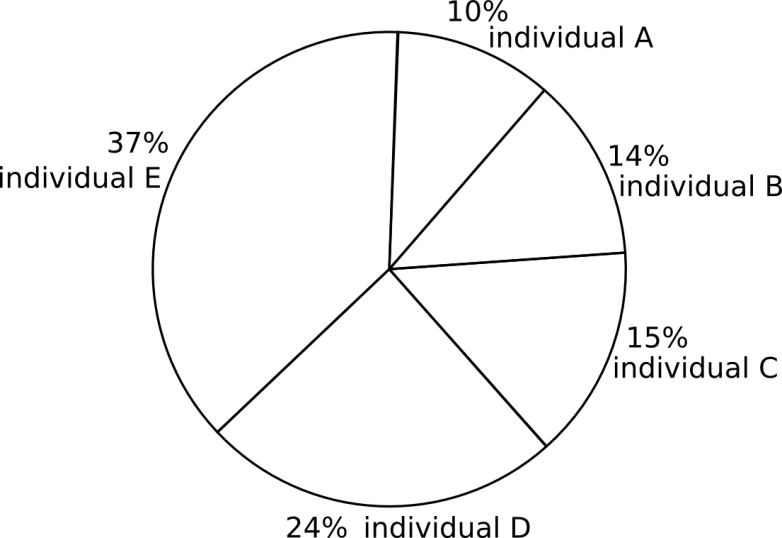
\includegraphics[width=0.7\linewidth]{chapters/genetic/rouletteWheel.png}
	\end{figure}
	
\end{algo}
\section{Anwendungsbereiche}
Ein theoretisches Anwendungsbeispiel ist das sogenannte Traveling-Salesman-Problem. Es geht dabei darum, dass ein Kaufmann von seinem Warenlager aus mehrere Stationen in einer Stadt beliefern und am Ende wieder zum Lager zurückkehren möchte. Dabei soll jede Station genau einmal besucht werden. Nummeriert man die Stationen mit 1 bis n durch, so erhält man eine Codierung für die Gene als Permutationen von 1 bis n. Die Fitnessfunktion ergibt sich dann als Kehrwert der Gesamtlänge des Weges. Bei der Reproduktion muss man jedoch vorsichtig sein, damit jedes mal gültige Permutationen entstehen. Dabei bietet es sich an eine Swap-Mutation durchzuführen. Die Kreuzung zweier Individuen erweist sich als komplizierter. Hier bietet es sich an ein Crossover durchzuführen, dann auf Gültigkeit zu testen und falls diese nicht vorhanden ist, das ganze rückgängig zu machen. Die entsprechenden Wahrscheinlichkeiten erhält man durch systematisches Probieren. Für die Selektion bietet sich dann die Ranked-Fitness-Selection an.

Genetische Algorithmen werden beispielsweise angewendet bei:
\begin{itemize}
	\item Konstruktion von komplexen Bauteilen
	\item Erstellung von Phantombildern
	\item Flugzeugbau
	\item Logistik (Ablaufplanung)
	\item Routenplanung
	\item Anordnungsprobleme
	\item Packprobleme
	\item Strategieprobleme (Spieltheorie)
	\item Parameteroptimierung
	\item Allgemein Optimierungsprobleme
\end{itemize}

Ein Beispielprogramm für die Logistik findet sich auf \href{http://www.dna-evolutions.com}{www.dna-evolutions.com}.

\section{Abgrenzung / Vergleich zu Neuronalen Netzen}
Ein Neuronales Netz ist ein Ansatz zur Lösung eines spezifischen Problems. Der Nachteil ist, dass man die Gewichte der einzelnen Knoten manuell durch Training anpassen muss. Genetische Algorithmen dagegen sind ein viel allgemeineres Prinzip, dass selbst optimale Lösungsansätze findet. So kann zum Beispiel auch ein genetischer Algorithmus verwendet werden, um ein neuronales Netz zu optimieren, oder sogar selbst zu entwerfen, indem er die Anzahl an Koten, Verbindungen und die Gewichte optimiert.\\

\section{Fazit \& Bewertung}
Genetische Algorithmen sind eine gute Möglichkeit um Optimierungsprobleme und Suchen mit großem Lösungsraum zu berechnen. Dabei werden im Gegensatz zu Expertensystemen keine weiteren Datenbanken oder ähnliches benötigt, sondern der Algorithmus verbessert sich immer weiter selbst. Der Nachteil ist, dass man in jedem  einzelnen Schritt stark vom Problem abhängige Wahlen treffen muss, die sich nicht unbedingt verallgemeinern lassen. Diese wirken sich dann stark auf den Ablauf des Programms aus und bestimmen das Ergebnis. Außerdem muss das Programm gegebenenfalls zur Laufzeit angepasst werden, entscheidet man  sich zum Beispiel das Selektionsverfahren zu ändern, damit eine Konvergenz des Algorithmus auftritt oder eine frühzeitige Konvergenz bei lokalen Maxima verhindert wird. Dennoch sind genetische Algorithmen eine sehr gute Alternative zum "`Brute Force"' Ansatz, da zum Finden einer Lösung nur ein kleiner Bruchteil des gesamten Lösungsraums betrachtet werden muss und das Programm mit einer gewissen Intelligenz nach einer Lösung sucht, anstatt blind alles auszuprobieren. Ein Problem bleibt jedoch, welches ist, dass immer nur eine Approximation und keine exakte Lösung berechnet wird. Daher muss man vorher abwiegen, ob dies ein guter Ansatz ist.

\section{Quellen und Literatur}

\href{http://www2.cs.uni-paderborn.de/cs/ag-klbue/de/courses/ws04/ea/students/ga_report.pdf}{(Skript Uni Paderporn)}\\
\href{http://www.mathematik.tu-dortmund.de/papers/MehmetiAmreinKulmsMacinLoenserBogonosWaidhas2014.pdf}{(Skript TU Dortmund)}\\
\href{http://www.spinfo.phil-fak.uni-koeln.de/fileadmin/spinfo/ki10/Genetische_algorithmen.pdf}{(Skript Uni Köln)}\\
\href{http://www.borgelt.net/slides/ga.pdf}{(Otto-von-Guericke-Universität )}\\
\href{http://www-e.uni-magdeburg.de/harbich/genetische_algorithmen/genetische_algorithmen.pdf}{(Skript Uni Magdeburg)}\\
\href{https://www.youtube.com/watch?v=kHyNqSnzP8Y}{(Vorlesung des MIT)}\\
\href{https://www.youtube.com/watch?v=6l6b78Y4V7Y}{(Vortrag von Kickstarter)}\\
\href{http://www.spektrum.de/lexikon/neurowissenschaft/zelle/14161}{(Spektrum Artikel zu Zellen)}\\
\href{http://www.spektrum.de/lexikon/biologie/genom/27365}{(Spektrum Artikel zu Genom)}\\
\href{http://semantic-web-grundlagen.de/w/images/e/e9/IntroAI-V06.pdf}{(Semantic Web)}\\
\href{http://comcute.eti.pg.gda.pl/wp-content/uploads/2012/12/image_9_5.png}{(Roulette-Wheel-Grafik)}\\
\href{http://janmonschke.com/Genetic-Algorithms/presentation/#/}{(Slides von Jan Monschke, TSP)}\\
\href{https://en.wikipedia.org/wiki/Tournament_selection}{(Tournament-Selection)}\\
Uiform-Fitness-Grafik von Denis Krzysztala\\


\part{Sensorik \& Interaktion}
\include{chapters/computervision/cv}
\include{chapters/sprachverarbeitung/sprachverarbeitung}

\part{Philosophische Grundlagen}
\include{chapters/intelligenzbegriff/begriff}
\chapterimage{chapter_head_1.png}

\chapter{Grenzen künstlicher Intelligenz}
\section{Motivation}
“The real risk with AI isn’t malice but competence.
A super-intelligent AI will be extremely good at accomplishing its goals, and if those goals aren’t aligned with ours, we’re in trouble.” (Stephen Hawking, 2015)

Der Begriff der künstlichen Intelligenz ist ein ebenso aktueller wie auch umstrittener Begriff, an dessen Definition sich schon seit Längerem die Geister scheiden.
Sie gilt als eine der zukunftsträchtigsten Forschungsthemen unserer Zeit.
So werden Methoden der künstlichen Intelligenz bereits erfolgreich in der Mustererkennung oder Computerspielentwicklung eingesetzt und stetig weiterentwickelt, um nur wenige Beispiele zu nennen.
Oft stellt sich dabei aber die Frage, wie weit die Kompetenzen einer KI gehen können bzw.
wie weit sie aus ethischer Sicht gehen sollten.
Denn neben den unstrittigen Vorteilen gibt es auch Vorbehalte und Ängste, wie das obige Zitat von Stephen Hawking deutlich macht.
Dieser spricht die Gefahren an, die entstehen könnten, wenn unsere Ziele nicht mit denen einer hoch entwickelten KI konform laufen.
Mit dieser Meinung steht Hawking nicht alleine da, denn mit Stuart J.Russell, Peter Norvig und Elon Musk unterschrieben im Jahr 2014 gleich mehrere Experten des Gebiets zusammen mit Hawking den „Open Letter on Artificial Intelligence“, in welchem vor den Gefahren einer unkontrollierbaren KI gewarnt und zu einer verantwortungsvollen Forschung in diesem Bereich aufgerufen wird.
Sind diese Bedenken berechtigt? Wie gefährlich bzw.
wie mächtig kann eine KI überhaupt sein? Inwiefern ähnelt sie der menschlichen Intelligenz und welche Stärken und Schwächen weist sie im Vergleich auf? Müssen wir uns vor einer Weiterentwicklung der KI fürchten, wie es manche Science-Fiction-Filme suggerieren oder liegt es an uns, sie zu kontrollieren und ihren Fähigkeiten Grenzen zu setzen?
Wieweit sollte man die Forschung in diesem Bereich aus ethischer Sicht vorantreiben?
Die folgende Ausarbeitung beschäftigt sich mit all diesen Fragen und versucht, einen Überblick über die Risiken und Grenzen künstlicher Intelligenz zu geben.

\section{Grenzen der Logik}
Methoden der künstlichen Intelligenz bedienen sich oft der Methoden der Logik, so wie es teilweise bei Bayesschen Netzen oder umfassender bei der automatischen Beweisführung geschieht.
Daher werden im Folgenden die Grenzen der Logik als Grundlage der künstlichen Intelligenz betrachtet.
Nennenswert ist in diesem Zusammenhang das Suchraumproblem.
Bei der Beweissuche gibt es für die Anwendung von Inferenzregeln in jedem Teilschritt unzählige bzw.
eventuell sogar unendlich viele Möglichkeiten, wodurch der Suchraum sehr schnell wächst.
Die Anwendung all dieser Möglichkeiten zur Beweisfindung ist für einen Menschen unzumutbar, während ein automatischer Beweiser tausende Inferenzen pro Sekunde durchführen kann.
Ein Mensch schafft u.~U.
eine Inferenz pro Sekunde.
Menschen inferieren also langsamer.
Überraschenderweise kann ein Mathematiker dennoch schwierigere Probleme schneller lösen als ein automatischer Beweiser.
Menschen können nämlich aufgrund ihrer Intuition und Anschauung mehrere, einfache Inferenzen des Beweisers in nur einem Schritt durchführen oder bereits bewiesene Lemmata benutzen, um sich Beweisschritte zu sparen, während ein maschineller Beweiser in jedem Schritt sehr viele Möglichkeiten ausprobiert, obwohl nur wenige zielführend sind.
Mittlerweile imitieren automatische Beweiser dieses menschliche Metawissen, sind aber bei Weitem nicht so effektiv wie ein erfahrener Mathematiker.
Unter anderem ist dies darauf zurückzuführen, dass Menschen bei komplexen Problemen zumeist selbst nicht in der Lage sind, ihre Intuition zu formalisieren.
Nicht formalisierbares Wissen kann in der Regel auch nicht programmiert werden, was den Möglichkeiten eines maschinellen Beweisers klare Grenzen setzt.

Eine andere Schwäche der Logik ist ihre Monotonie.
Das bedeutet, dass mit der Erweiterung der Formelmenge zwar neue Aussagen bewiesen werden können, alle zuvor ableitbaren Formeln aber nach wie vor bewiesen werden können, sodass die Menge der ableitbaren Aussagen monoton wächst.
Dieser Umstand kann allerdings zu Widersprüchen führen.
Am Beispiel des "`fliegenden Pinguins"' kann diese Problematik ganz einfach illustriert werden:
Angenommen man weiß, dass Tweety ein Pinguin ist, Pinguine Vögel sind und Vögel fliegen.
Daraus lässt sich per Resolutionsbeweis ableiten, dass Tweety fliegen kann.
Da Pinguine aber nicht fliegen können, fügt man eine Regel hinzu, die besagt, dass Pinguine nicht fliegen.
Daraus lässt sich ableiten, dass Tweety nicht fliegen kann.
Es lässt sich aus dieser Wissensbasis aber nach wie vor auch ableiten, dass Tweety fliegen kann, da die neue Regel die bestehenden Regeln nicht ersetzt, sondern erweitert.
Wenn man nun die Wissenbasis um die prädikatenlogische Formeln "`Abraxas ist ein Rabe"' und "`Raben sind Vögel"' ergänzt, kann man nicht mit Sicherheit darauf schließen, dass Abraxas fliegen kann, da keine Aussage darüber gemacht wird, ob Abraxas ein Pinguin ist oder nicht.
Um das Problem zu lösen, müsste die Tatsache "`Abraxas ist kein Pinguin"' hinzugefügt werden, während dies für einen Menschen einen selbstverständlichen Fakt darstellt.
Wie man an diesem Beispiel sehen kann, muss für jedes Objekt in der Wissensbasis nicht nur angegeben werden, welche Merkmale es besitzt, sondern auch welche es nicht besitzt.
Für ein komplexeres Problem impliziert dies ein explosionsartiges Wachstum des Programmieraufwands, wenn die Wissensbasis erweitert oder verändert wird.

Weiterhin ist festzustellen, dass mit der Prädikatenlogik eine Reihe von Aussagen nicht formuliert werden kann, da z.~B.
Quantoren für Funktionen nicht eingesetzt werden dürfen.
Logiken
höherer Stufen bieten diese gewünschten Erweiterungen, allerdings hat Gödel gezeigt, dass
schon eine minimale Erweiterung der Prädikatenlogik zum Verlust der Vollständigkeit führt, d.~h.
es gibt wahre Formeln, die nicht beweisbar sind.
Folglich sind die Prädikatenlogik wie auch Logiken höherer Stufen noch nicht mächtig genug.
Außerdem ist es fraglich, ob etwas derart Komplexes wie das menschliche Denken bzw.
Verhalten durch eine Menge von Formeln beschrieben werden kann.
In der Regel ist es nicht möglich, die menschliche Intelligenz umfassend in Formeln auszudrücken, was auch als Qualifizierungsproblem bezeichnet wird.
Das Problem liegt darin, dass Menschen nicht in Formeln denken oder anhand von Formeln Entscheidungen treffen, sondern implizit den gesamtheitlichen Kontext betrachten und davon abhängig handeln.
Sie haben einen Sinn dafür, wie in einer Situation zu verfahren ist bzw.
was man für ein Verhalten erwarten würde, so wie es bspw.
der Fall ist, wenn man ein Geschenk erhält und dann den Drang empfindet, selbst etwas an den Schenker zu verschenken.
Insgesamt kann man also festhalten, dass die Logik als Grundlage einer künstlichen Intelligenz dem menschlichen Verstand in vielerlei Aspekten trotz Imitationsversuchen noch weit unterlegen ist.

\section{Experimente}
Sehr wichtig für das Thema dieser Arbeit sind Experimente und Tests, die zum Ziel haben, eine intelligente Maschine als solche einzustufen, denn anhand dessen kann festgestellt werden, wie nah eine KI der menschlichen Intelligenz ist und wo ihre Grenzen liegen.
Der Turing-Test ist der wohl bekannteste Versuch.
Dabei sitzt eine Person A in einem Raum an zwei Computern, über die sie Fragen eintippen kann, wobei ein Computer mit der vermeintlichen künstlichen Intelligenz und der andere Computer mit einer weiteren Person B verbunden ist.
Nach fünf Minuten muss A entscheiden, mit welchem Computer die KI verbunden ist.
Wenn A in 30\% aller Fälle falsch entscheidet, besteht die Maschine den Test und weist somit intelligentes Verhalten auf.
Mittlerweile gibt es eine Reihe von sogenannten Chatterbots, die zu Beginn einer Konversation überraschend oft passgenaue Antworten liefern.
Bekannt und besonders effektiv in der Täuschung sind z.~B.
Eliza oder Mgonz, aber auch CyberLover.
Letzterer geht bereits soweit, dass er seinem Gesprächspartner persönliche Daten zu entlocken versucht, um seine Identität festzustellen und diese zu stehlen.
Diese Programme offenbaren aber im Laufe des Gesprächs relativ schnell ihre begrenzten Antwortmöglichkeiten, da sie entweder nicht lernfähig sind oder nur einen auf bestimmte Bereiche beschränkten Wissensstand aufweisen.
Dies erkennt man sehr gut am folgenden Beispiel einer in das Deutsche übersetzten Konversation mit Eliza:

\begin{verbatim}
ELIZA: Wie geht es Ihnen.
Bitte schildern Sie Ihr Problem.
Ich verbringe zu viel Zeit am Computer.
ELIZA: Warum erwähnen Sie Computer?
Du bist einer.
ELIZA: Macht es Ihnen Spaß zu glauben, ich sei einer?
Ja.
ELIZA: Sie scheinen sehr optimistisch zu sein.
Bin ich.
5
ELIZA: Wie lange sind Sie schon?
31 Jahre.
ELIZA: Ich bin mir nicht sicher, ob ich sie verstehe.
Willkommen im Club
ELIZA: Bitte fahren Sie fort.
Was du sagst, ist auch nicht sehr sinnvoll.
ELIZA: Wir reden über Sie, nicht über mich.
\end{verbatim}

Man sieht an diesem Beispiel relativ klar, dass Eliza zunehmend verwirrende Antworten gibt, je einfältiger die Antworten des Kommunikationspartners von Eliza ausfallen.
Der noch blamablere Fall von TayTweets verdeutlicht um einiges besser die fehlende Intelligenz der derzeitigen Chatterbots.
Turing prognostizierte seinerzeit, dass ein Computer im Jahr 2000 den Test besteht.
Diese Vermutung hat sich noch nicht bewahrheitet, da Computer heute einiges leisten können, die Führung einer offenen Konversation aber derzeit nicht dazugehört.
Zurückzuführen ist dies darauf, dass der Mensch ein immenses Hintergrundwissen besitzt, wodurch die Menge an möglichen Fragen eine intelligente Maschine schier überfordert.
Es gab zwar einen Fall einer russischen Software, die den Test bestanden hat.
Allerdings wurden Mängel am Versuchsaufbau und an den Fragen der Jury festgestellt.
Was den Turing-Test aber so interessant macht, ist die Frage, ob damit ein maschinelles Denken nachgewiesen werden kann.
Es gibt Meinungen, die behaupten, dass der Turing-Test höchstens die Simulation des Denkens und nicht das Denken selbst nachweisen kann.
Es wird an dem Test kritisiert, dass der Computer die Ein- und Ausgaben nicht wirklich versteht und lediglich richtige Antworten gibt, weshalb man nicht von einer Darstellung von Verstand sprechen kann.
Versuche, den Test zu bestehen, waren darüber hinaus eher darauf ausgerichtet, den Kommunikationspartner zu überlisten und nicht darauf, eine zu einer Konversation fähige, echte Intelligenz zu entwickeln.

Ebenso wie die Kritik am Turing-Test setzt das Experiment "`Chinese Room Experiment"' von John R.
Searle am Verständnis an.
Dabei sitzt eine Versuchsperson, die nur Englisch versteht, in einem Raum mit einer kleinen Öffnung.
Ausgestattet ist sie dabei mit einem in englischer Sprache verfassten Regelbuch mit Anweisungen sowie mit mehreren teils leeren, teils mit für die Versuchsperson nicht entzifferbaren Aufschriften versehenen Papierstapeln.
Über die Öffnung erhält er von außen Papierstreifen mit unbekannten Symbolen.
Die Versuchsperson sucht diese Zeichen im Regelbuch, führt die einschlägigen Anweisungen durch und muss dafür gegebenenfalls die Papierstapel nach Symbolen durchsuchen oder Symbole auf leere Papierstreifen schreiben.
Am Ende jeder Anweisung muss ein Papierstreifen beschrieben und über die Öffnung nach außen durchgereicht werden.
Außerhalb des Raums werden die Papierstreifen von einem chinesischen Muttersprachler beschrieben und über die kleine Öffnung in den Raum gegeben.
Man erhält dann nach einer gewissen Zeit einen Papierstreifen aus dem Inneren des Raums, wobei dieses mit einer passgenauen, in chinesischer Sprache verfassten Antwort zu dem zuvor hineingegebenem Papierstreifen beschriftet ist.
Der chinesische Muttersprachler schließt daraus, dass sich ein chinesisch sprechender Mensch im Raum aufhält.
In diesem Fall verstehen weder die Versuchsperson noch das Regelbuch oder die Papierstapel Chinesisch, erzeugen zusammen aber über Vergleiche der Schriftzeichen Antworten, wie es der Turing-Test erfordert.

Searle wollte damit zeigen, dass die Ausführung des richtigen Programms ohne die Erzeugung eines Verständnisses auskommt, weshalb auch eine KI seine Ein- und Ausgaben nicht verstehen muss, um nach Turing als intelligent zu gelten.
So wollte er als Kritik am Turing-Test verdeutlichen, dass man nie feststellen kann, ob eine Maschine Verstand bzw. Verständnis besitzt.
Ein neueres Unterfangen ist der Lovelace-2.0-Test von Mark O.
Riedl, welcher als Kritik am Turing-Test entstand.
Eine Konversation zu führen, verkörpere keine wahre Intelligenz.
Diese bestünde stattdessen in der Kreativität.
Diesem vorangegangen war der einfache Lovelace-Test, welcher die kreative Schöpfung von etwas Neuem als einziges Indiz für Intelligenz sieht.
Dieser Test wurde abgeändert, da er impliziert, dass das Werk der KI nur als kreativ gewertet werden kann, wenn der Entwickler der KI die Entstehung des Werks nicht versteht.
Da es deshalb nahezu unmöglich gewesen wäre, diesen Test zu bestehen, erfand Riedl den Lovelace-2.0-Test.
Hierbei wird die KI aufgefordert, zu einem vorgegebenen Thema eine Geschichte zu erzählen.
Wenn die KI dies schafft, wird das Thema immer weiter eingegrenzt und die KI immer wieder aufgefordert, eine Geschichte zu erzählen, bis die KI es nicht mehr schafft.
Damit kann man das Ausmaß der Intelligenz einer Maschine einordnen.
Die Programme von Riedl selbst haben nur die ersten zwei Stufen des Tests bestanden, was für ein niedriges Maß an Intelligenz spricht, da ein Autor oder Dichter erst an weitaus höheren Stufen scheitern würde.
Auch dieser Test zeigt also die Begrenztheit der aktuellen KI-Programme.

\section{Unfähigkeit}
Die herrschende Meinung in der Gesellschaft zum Thema "`künstliche Intelligenz"' besagt, dass Maschinen trotz aller Fortschritte zu bestimmten Dingen nicht fähig sind und in absehbarer Zeit auch nicht sein werden.
Turing listete in einem ganzen Katalog solche Dinge auf, zu denen beispielsweise "`etwas wirklich Neues tun"', "`initiativ sein"', "`Fehler machen"', "`verlieben"' oder "`Erdbeereis mit Sahne mögen"' zählen.
Zwar können sich Computer nicht verlieben, wie es Filme/Romane in Bezug auf die Liebe zwischen Mensch und Maschine seit jeher prophezeien.
Allerdings ist es geradezu erstaunlich, wie viel Computer von dem Katalog von Turing bereits können bzw.
besser können als Menschen.
Ein Beispiel ist, dass Computer ebenso wie der Mensch Fehler machen, sodass man diesen Punkt aus dem oben genannten Katalog streichen kann.
Es gibt sogar Fälle, in denen ein Computer ungeduldig werden kann.
Es bleibt alles in allem dennoch dabei, dass Maschinen in bestimmten Dingen an ihre Grenzen stoßen.
Menschen haben beispielsweise die Fähigkeit, einen unbekannten Raum zu betreten, sofort die Szene zu erfassen, darauf aufbauend Aktionen zu planen und Entscheidungen zu treffen.
Zurückzuführen ist dies auf das Adaptivitätsmerkmal der Menschen, sie passen sich an verschiedenste Umweltbedingungen an und ändern ihr Verhalten, indem sie lernen.
Diese Anpassungsfähigkeit und das ausgeprägte Lernverhalten fehlt den Maschinen, wobei man sich dem letzteren zunehmend durch die Nutzung von Methoden des Machine Learning annähert.

Ähnlich verhält es sich mit der Sprache.
So spricht Noam Chomsky den Maschinen die
Sprachkompetenz ab, da den Menschen nicht erlernbare sprachliche Fähigkeiten angeboren seien, die es erlauben, noch nie gehörte, komplexe Sätze hervorzubringen.
Den Menschen sei eine universelle Grammatik in die Wiege gelegt, anhand derer die Nutzung und das Erlernen von Sprache möglich sei.
Maschinen sind darüber hinaus nicht in der Lage, Dinge aus eigenem Antrieb hervorzubringen und spontan zu handeln.
Vielmehr führen sie Anweisungen auf gegebenen Daten aus, wenn eine bestimmte Bedingung erfüllt ist, was nicht für die Existenz einer Intelligenz spricht.
Menschen haben weiterhin ein Bewusstsein, d.~h.
sie können über sich selbst nachdenken oder darüber, dass sie über sich selbst nachdenken können usw.

Dies ist der ausschlaggebende Unterschied zwischen dem Menschen und einer künstlichen Intelligenz.
Es reicht also bspw.
nicht, ein Gedicht zu schreiben, sondern es muss einem bewusst sein, dass man das Gedicht geschrieben hat.
Einem KI-Programm fehlt es zusätzlich an Emotionen, allen voran an Empathie, die über die bloße Einschätzung des Gefühlszustands des Gegenübers hinausgeht und in der Regel in einer emotionalen Reaktion besteht.
Zuletzt ist festzustellen, dass bisher kein Programm die Leistung des menschlichen Gehirns bei einem derart niedrigen Energieverbrauch auch nur annähernd erreicht hat.

Wie man sieht, gibt es noch eine Reihe an Dingen, die intelligente Maschinen nicht beherrschen, aber auch Fähigkeiten, die sie im Laufe der Zeit dazugewonnen haben.
Unfähigkeit von Computern ist also ein generisches Problem.
Was eine künstliche Intelligenz heute nicht kann, macht sie morgen vielleicht um ein Vielfaches effizienter als ein Mensch.

\section{Ethische Aspekte und Risiken}
Eine weitere Frage nach den Grenzen der künstlichen Intelligenz ist die, ob man künstliche Intelligenzen vor dem Hintergrund moralischer Aspekte weiterentwickeln sollte.
Die Forschung steht im Falle einer Weiterentwicklung vor dem Problem der unvorhersehbaren, möglicherweise negativen Konsequenzen.
Die Erfindung der Kernspaltung, die unter anderem zur Katastrophe von Tschernobyl führte, oder des Verbrennungsmotors, welcher zur globalen Erwärmung und Luftverschmutzung maßgeblich beiträgt, wird dabei als negatives Vergleichsbeispiel gesehen.
Eine Befürchtung ist der Verlust von Arbeitsplätzen bei einer fortschreitenden Automatisierung.
Beispielsweise werden in den USA manche Kreditkartenanwendungen und die Erkennung von Kreditkarten-Betrug von Programmen aus der künstlichen Intelligenz ausgeführt.
Es liegt also die Vermutung nahe, dass in diesem konkreten Fall Arbeitsplätze verloren gegangen sind.
Dem ist aber in der Regel nicht so, da diese Arbeitsplätze gar nicht existieren würden, weil sie für das Unternehmen nicht wirtschaftlich wären.
So hat eine Bank in der Regel keinen Mitarbeiter, der nur Kreditkartenbetrug aufdeckt.
Es geht also auch kein Arbeitsplatz verloren, wenn eine künstliche Intelligenz diese Aufgabe übernimmt.
Dieses Beispiel kann man auf die meisten Fälle übertragen, in denen eine KI bestimmte Leistungen bietet.
Aber angenommen, die Arbeitslosigkeit würde steigen.
Dann würde das Bruttosozialprodukt eines Landes dennoch nicht sinken bzw.
sogar steigen, da die Wertschöpfung durch den Einsatz von effizienteren Maschinen steigen
würde.
Die arbeitslos gewordenen Menschen würden dann womöglich durch die Verteilung
des neu hinzugewonnenen Reichtums bedient werden, weshalb sich die Arbeitslosigkeit nicht unbedingt negativ auswirken müsste.
Falls es aber gelingt, hochintelligente Maschinen zu entwickeln, die alle Aufgaben der Menschen im Beruf oder im Haushalt übernehmen können, wäre es durchaus denkbar, dass es überhaupt keine von Menschen zu verrichtende Arbeit mehr gibt, die Menschen in hohem Maß von den Maschinen abhängig sind und sie daher keinerlei Druck verspüren bzw.
keinerlei Anstrengungen für ihre Existenz unternehmen, sodass es zu einem gesellschaftlichen Kollaps kommen kann.

Als eine weitere mögliche Gefahr wird in der Literatur oft der Umstand genannt, dass eine sehr weit entwickelte KI dem Menschen sein Selbstverständnis als einzigartiges Individuum rauben kann und ihm somit das Gefühl eines imitierbaren, lediglich in einem System funktionierenden Automaten vermittelt.
Diese Gefahr ist allerdings zu relativieren, denn in der Geschichte gibt es viele ähnliche Beispiele, die dem Menschen ihr Einmaligkeitsgefühl streitig machten.
So stellte Darwin mit seiner Evolutionstheorie den Menschen auf eine Stufe mit den Tieren, was seinerzeit umstritten war, jedoch bis dato nicht zu einem Verlust jenes Selbstverständnisses geführt hat.
Zudem macht es den Menschen wiederum zu etwas Besonderem, wenn er in der Lage ist, eine der menschlichen Intelligenz ähnliche Intelligenz künstlich zu erschaffen.

Darüber hinaus könnte die zunehmende Automatisierung durch Programme der künstlichen Intelligenz bewirken, dass man sich seiner Verantwortung entzieht.
Haftet beispielsweise der Arzt, wenn eine KI eine falsche medizinische Diagnose liefert? Wem sind Schulden zuzuordnen, wenn eine KI, die Geldgeschäfte für ein Unternehmen erledigt, diese ohne weitere Nachfrage aufgenommen hat? Diese Frage wird umso relevanter werden, je stärker die Automatisierung voranschreitet.

Auch begründet ist die Sorge nach dem Einsatz von künstlicher Intelligenz zu unerwünschten Zwecken.
Mit diesem Problem ist man derzeit im Militär konfrontiert, bspw.
nutzten die USA im Irakkrieg über 5000 unbemannte, autonome Luftfahrzeuge, mit denen Menschen umgebracht werden konnten, ohne dass je ein Mensch sein Leben aufs Spiel setzen musste.
Zudem stellt sich für den Menschen dann gar nicht die Frage nach der moralischen Verwerflichkeit seines Handelns, da er außer Reichweite ist und nicht merkt, was sein Handeln für Konsequenzen hat.

Ein anderes Problemgebiet ist das Potenzial der künstlichen Intelligenz über die Spracherkennung die Privatsphäre der Menschen zu verletzen.
Ihr ist zu verdanken, dass Staaten mittlerweile regelmäßig Telefongespräche abhören.
Eine KI kann also leicht opportunistisch genutzt werden, wenn sie in die falschen Hände gerät.
Einige Meinungen gehen sogar so weit, dass sie einer KI die Fähigkeit einräumen, das Ende der Menschheit herbeizuführen.
Es ist durchaus umstritten, ob diese Einschätzung realistisch ist oder nur in der Fiktion eintreten kann.
Die falsche Zustandsabschätzung einer KI kann zu erheblichen Schäden führen.
Beispielsweise könnte ein autonomes Raketenabwehrsystem eine Bewegung im Luftraum fälschlicherweise für einen Angriff halten und entsprechend reagieren, sodass es zu einem Verlust von Menschenleben kommen kann.
Allerdings besteht dieses Risiko auch stets, wenn ein Mensch das System bedienen würde, sodass das Problem nicht nur auf eine KI zurückzuführen ist.

Weiterhin kann es sein, dass die Nutzenfunktion einer KI, nach der sie letztlich handelt, fehlspezifiziert ist.
Sie könnte bspw.
derart programmiert werden, dass sie das menschliche Leid zu minimieren versucht.
Der Mensch neigt nun aber dazu, sich immer wieder beabsichtigt oder unbeabsichtigt neue Situationen des Leidens zu schaffen.
Die vermeintliche Konsequenz
wäre mit der oben genannten Nutzenfunktion als Handlungsrahmen die Ausrottung der
Menschen.
Dies suggerieren bisweilen auch viele Science-Fiction-Filme.
Was hier aber implizit angenommen wird, ist zum einen die Tatsache, dass die KI die Nutzenfunktion zu wörtlich nimmt, und zum anderen die Aggressivität, die eine Maschine nicht unbedingt aufweisen muss, dem Menschen aber im Zuge der natürlichen Selektion in die Wiege gelegt ist.
Außerdem sollte erwartet werden können, dass eine Maschine, die eine derartige Intelligenz besitzt, dass sie den Menschen als bis dato intelligentestes Lebewesen auszulöschen in der Lage ist, auch die Intelligenz besitzt, die Absicht der Nutzenfunktion richtig zu deuten.

Gefährlicher ist dagegen eine statische Nutzenfunktion, da sie nur die Werteverhältnisse der Entstehungszeit einer KI umfassen kann.
So würde eine KI, die im 18.
Jahrhundert entwickelt wurde, heute versuchen, das Wahlrecht für Frauen abzuschaffen und damit aktuelle Moralvorstellungen untergraben, anstatt diese zu fördern.
Sinnvoller erscheint dagegen, dass die KI ihre Nutzenfunktion selbst aktualisiert.
Hier bestünde aber die Gefahr, dass die Maschine tiefste Abgründe des menschlichen Denkens erkennt und entsprechend handelt.
Beispielsweise könnte sie erkennen, dass Menschen keine Scheu haben, lästige Insekten zu töten, weil letztere als primitiv angesehen werden.
Sie würde daher womöglich das Töten von Menschen für moralisch unverwerflich halten, da diese wiederum im Vergleich zu ihr primitiv sind.
Nimmt man nun aber an, dass eine hoch entwickelte KI nicht aggressiv ist, so gibt es auch dann problematische Punkte, die zu beachten sind.
Wenn die Intelligenz einer Maschine die des Menschen übersteigt, so wird insbesondere sie in der Lage sein, eine noch weiter entwickelte Intelligenz hervorzubringen und letztere wird genauso verfahren, sodass es irgendwann zu einer sogenannten Intelligenzexplosion, auch als technologische Singularität bezeichnet, kommt und der Mensch im Vergleich zu den Maschinen zu einem primitiven Wesen verkommt.
Dadurch würde der Mensch zwar nicht unbedingt im physischen Sinne bedroht werden, allerdings würde er die Entwicklung vom Herrscher über die Erde zum Beherrschten vollbringen, so wie einst mit der Evolution des Menschen die Ära der Tiere endete.
KI könnten dann die Entwicklung der menschlichen Zivilisation lenken.

Dieses Szenario wird allerdings nicht ausschließlich negativ aufgenommen.
Mit dem Transhumanismus gibt es eine Bewegung, die sich das Zusammenleben und die Zusammenarbeit von Mensch und Maschine herbeiwünscht, wobei einige sogar dem Ersatz des Menschen durch die Maschine entgegenfiebern.
Ray Kurzweil ist der bekannteste Anhänger dieser Meinung.
Er sieht hierin die Möglichkeit für den Menschen, über seine eigene Sterblichkeit zu entscheiden, indem die Grenzen des menschlichen Körpers gesprengt werden.
Die KI könnten als nächste Evolutionsstufe des Menschen gesehen werden.
Man solle aber die Ur-KI so programmieren, dass sie den Menschen gut behandelt, denn dann würden es ihr die von ihr entwickelten, intelligenteren Programme gleichtun, sodass keinerlei Gefahren für die Menschheit bestehen würden.

\section{Grenzen der Hardware}
Der Folgende Abschnitt befasst sich nur mit den Grenzen des Prozessors.
Aktuell wird die Grenze der Leistungsfähigkeit einer CPU durch die Anzahl der Transistoren auf den Prozessoren, sowie die Anzahl der Prozessoren festgelegt.
Das Wachstum der Transistoranzahl auf einem Chip konnte in den letzten knapp 100 Jahren durch das Mooresche Gesetz beschrieben werden.

Das Moorsche Gesetz besagt, dass sich die Komplexität integrierter Schaltkreise mit minimalen Komponentenkosten regelmäßig verdoppelt, also verdoppelt sich die Anzahl der Transistoren auf einem Chip alle 12 bis 18 Monate (je nach Quelle) auf einer CPU.
Da die Größe eines Chips begrenzt ist muss folglich die Größe der Transistoren abnehmen.

\subsection{Fertigung einer CPU}

Bei der Abnahme der Transistorgröße gibt es allerdings einige Limitierungen wie z.B. wirtschaftliche Effizienz, da es immer aufwendiger wird in zunehmend kleineren Dimensionen Transistoren auf dem Chip aufzubringen,
und das Auftreten von Quantenmechanischen Effekten, bei denen Elektronen, welche zum Ladungstransport innerhalb eines Transistors benutzt werden,
Aufenthaltswahrscheinlichkeiten außerhalb des Transistors besitzen und folglich den Zustand des Transistors verfälschen.
Diese Quantenmechanischen Effekte treten ab einer Fertigungsgröße von 5nm auf, welche auch als die \enquote{Magische Grenze} bekannt ist.

Aktuell liegen die Fertigungsgrößen bei etwa 14nm bei der Skylake Architektur von Intel, diese CPUs werden mit einem Verfahren namens EUV-Lithografie hergestellt. Die EUV-Lithografie benutzt weiche Röntgenstrahlung,
welche frei wird wenn man auf ein bestimmtes Gasgemisch mit einem Laser strahlt, um die Transistoren auf der Oberfläche des Chips zu befestigen.


\subsection{Alternativen für die Zukunft}

Folglich gibt es eine Leistungsgrenze für Prozessoren, daher wurden für die Zukunft Alternativen gesucht.
Aktuell sind die vielversprechendsten Alternativen, Quantencomputer und DNA-Computer, welche bei bestimmten Problemstrukturen bis zu 100 Mio mal so schnell sind wie die heutige Durchschnittscomputer.
Dennoch haben auch Quantencomputer schwächen wie Beispielsweise die sehr aufwändige Kühlung des Q-Bits auf 3 Grad Kelvin.
Quantencomputer bergen auch ein gewisses Risiko, da sie Aufgaben wie die Primfaktorzerlegung, auf welcher fast alle Modernen Verschlüsselungen basieren, binnen wenigen Sekunden durchführen können.
DNA-Computer haben das Problem, dass die Ergebnisse welche sie ausgeben noch von einem Computer interpretiert werden müssen, was extrem aufwändig ist.

\section{Fazit}
Insgesamt kann man festhalten, dass Errungenschaften der KI-Forschung uns derzeit diverse Erleichterungen bieten und sich dieser Trend in Zukunft sogar verstärken wird.
Nichtsdestotrotz sind die Möglichkeiten von Programmen der KI begrenzt.
So sind Computer möglicherweise effizienter als der Mensch, aber nicht unbedingt auch effektiver.
Vom mathematisch-logischen Standpunkt aus betrachtet, können Computer viele Berechnungen und Inferenzen sehr schnell durchführen.
Wenn aber ein komplexeres Problem vorliegt, kann der Mensch durch seine Intuition bzw.
sein Metawissen im Vergleich zum Computer schnellere Schlüsse ziehen.
Auch generell gibt es bestimmte Fähigkeiten, die eine KI zumindest noch nicht beherrscht.
So besitzen Maschinen kein Bewusstsein und sind nicht fähig, Emotionen zu empfinden.
Diverse Tests und Experimente verdeutlichen, dass maschinelles Denken und Verstehen nicht unbedingt nur aus der Angabe von passenden Antworten in einer Konversation abgeleitet werden kann.
Man kann zudem festhalten, dass einige Sorgen bezüglich der Macht einer KI schlicht unberechtigt sind, da bisher keine Fälle von gefährlichen, unkontrollierbaren Ereignissen auftraten.
Auch ist die instinktiv angenommene Bösartigkeit und Aggressivität einer intelligenten Maschine kein Pflichtmerkmal, sondern eher eine Eigenschaft der dystopischen Fiktion.
Andere Sorgen finden dagegen durchaus Berechtigung.
Dazu zählen vor allem Risiken ethischer Natur.
Es könnte bspw.
zu einem Wandel der gesellschaftlichen Struktur kommen, je mehr intelligente Maschinen uns Aufgaben abnehmen und somit den Standardlebenszyklus Arbeit-Konsum untergraben.
Problematisch könnte weiterhin die Spezifikation der Wertevorstellungen und der Nutzenfunktion einer KI sein, damit eine KI im Sinne ihres Schöpfers handelt.
Es bleibt abzuwarten, welche der Risiken tatsächlich eintreten werden.
Dennoch sollte wie in jedem anderen Bereich Wert auf eine verantwortungsvolle Forschung gelegt werden, insbesondere in den Fällen, in denen eine KI Menschenleben gefährden könnte, wie es bspw.
bei autonomen Luftabwehrsystemen der Fall ist.
Man sollte sich zum Thema KI nicht allzu sehr von der Fiktion irritieren lassen.
Entgegen der Meinungen bekannter Persönlichkeiten wie Elon Musk oder Stephen Hawking ist festzustellen, dass KI-Programme noch nicht in der Lage sind, eine ernsthafte Gefahr für den Menschen darzustellen.
Es ist zumindest zu früh, sich Weltuntergangsszenarien auszumalen, da zum derzeitigen Forschungsstand viele der in diesen Szenarien typischerweise auftretenden Fähigkeiten der Maschinen klar und deutlich außerhalb des Machbaren liegen.
In absehbarer Zeit scheint ein Ende der Welt durch die Hand einer KI nicht wahrscheinlicher zu sein als durch die Handlungen der Menschen selbst.

\section{Literatur}
\begin{itemize}
\item Wolfgang Ertel, Grundkurs Künstliche Intelligenz – Eine praxisorientierte Einführung, 2013 (3.Auflage), Springer-Verlag.
\item Stuart Russell \& Peter Norvig, Künstliche Intelligenz – Ein moderner Ansatz, 2012 (3.Auflage), Pearson-Verlag.
\item Karsten Hartmann, Einführung in die Expertensystem-Technologie, 2015, Hochschulverlag Merseburg.
\item Nils J.
Nilsson, Die Suche nach künstlicher Intelligenz – Eine Geschichte von Ideen und Erfolgen, 2014, AKA-Verlag.
\item \url{http://www.wired.com/brandlab/2015/10/stephen-hawkings-ama/}
\item \url{https://www.wired.de/collection/featured/ein-neuer-test-soll-nachweisen-wie-intelligent-computerprogramme-sind}
\item \url{http://www.netzpiloten.de/emotionen-kuenstliche-intelligenz-ki/}
\item \url{http://www.faz.net/aktuell/feuilleton/debatten/warum-die-kuenstliche-intelligenz-gefahren-birgt}
\item \url{https://en.wikipedia.org/wiki/Open_Letter_on_Artificial_Intelligence}
\end{itemize}


\part{Appendix}

\defbibfilter{papers}{
  type=article or
  type=inproceedings
}

\chapter*{Literaturverzeichnis}
\addcontentsline{toc}{chapter}{\textcolor{hhublue}{Literaturverzeichnis}}
\section*{Bücher}
\addcontentsline{toc}{section}{Bücher}
\printbibliography[heading=bibempty,type=book]
\section*{Wissenschaftliche Artikel}
\addcontentsline{toc}{section}{Wissenschaftliche Artikel}
\printbibliography[heading=bibempty,filter=papers]
\section*{Webpages}
\addcontentsline{toc}{section}{Webpages}
\printbibliography[heading=bibempty,type=online]

%----------------------------------------------------------------------------------------
%	INDEX
%----------------------------------------------------------------------------------------

\cleardoublepage
\phantomsection
\setlength{\columnsep}{0.75cm}
\addcontentsline{toc}{chapter}{\textcolor{hhublue}{Index}}
\printindex

%----------------------------------------------------------------------------------------

\end{document}
